\documentclass[12pt, titlepage]{scrartcl}

\usepackage[ngerman]{babel}
\usepackage[ansinew]{inputenc}
\usepackage{color}
\usepackage[a4paper, lmargin={2.5cm}, rmargin={2cm}, tmargin={2.5cm}, bmargin={2.5cm}]{geometry}
\usepackage{amssymb}
\usepackage{amsthm}
\usepackage{graphicx}
\usepackage{booktabs}
\usepackage{float}
\usepackage{array}
\usepackage{adjustbox}
\usepackage{longtable}
\usepackage{booktabs}

\newcommand{\RN}[1]{%
	\textup{\uppercase\expandafter{\romannumeral#1}}%
}

\newcommand{\Abb}[1]{%
	Abb.\ \ref{#1}%
}

\renewcommand{\arraystretch}{1.2}

\usepackage{scrpage2}
\pagestyle{scrheadings}
\clearscrheadfoot

\ofoot{\pagemark}
\ifoot{RBSG - Enhanced Wars}
\cfoot{Gruppe G}
\ohead{
\includegraphics[width=0.12\textwidth]{Logo.png}}

\begin{document}
	\begin{titlepage}
		\centering
		% \includegraphics[width=0.15\textwidth]{example-image-1x1}\par\vspace{1cm}
		{\scshape\LARGE Universtit�t Kassel \par}
		\vspace{1cm}
		{\scshape\Large Projektdokumentation\par}
		\vspace{1.5cm}
		{\huge\bfseries RBSG - Release \RN{2}\par}
		\vspace{2cm}
		{\scshape\Large Software Engineering \RN{1} SS19\par}
		\vspace{0.5cm}
		{\scshape\Large Gruppe G\par}
		\vspace{0.5cm}
		{\Large\itshape Scrum Master: Juri Lozowoj\par}
		\vspace{0.5cm}
		{\Large\itshape Product Owner: Georg Siebert\par}
		\vspace{2cm}
		{
\includegraphics[width=1\textwidth]{Logo.png}\par}
		\vfill
		% supervised by\par
		% Dr.~Mark \textsc{Brown}
	\vfill
	
	% Bottom of the page
	{\large \today\par}
	\end{titlepage}
	\begin{abstract}
		Diese Dokumentation beschreibt das zweite Release des Projektes RBSG von Team G. Dies umfasst die Auflistung und Erl�uterung der Mockups und der Domain Stories. Beide Sprints werden dokumentiert und analysiert. Zum Schluss wird das Resultat des Releases mit den Zielen verglichen und es wird auf  Probleme oder nicht erf�llte Anforderungen eingegangen.
	\end{abstract}
	\pagenumbering{Roman}
	\tableofcontents
	\newpage
	\pagenumbering{arabic}
	\setcounter{page}{1}
	\section{Ziel der Dokumentation}
		Die Dokumentation soll den Verlauf des Entwicklungsprozesses des Spiels RBSG f�r das zweite Release veranschaulichen und analysieren. Dies umfasst die Entstehung der Mockups und Domain Stories, welche die Grundlagen f�r die Entwicklung bilden. Es werden f�r alle Sprints das Sprintziel, die User Stories sowie eine Analyse des Sprintverlaufs erstellt. Abschlie�end werden die Mockups mit den Ergebnissen des Sprints verglichen. Dabei wird darauf eingegangen, wieso Features anders Umgesetzt oder weggelassen wurden.
	\section{Das Projekt RBSG}
			Das Projekt RBSG findet im Rahmen der Veranstaltung Software Engineering \RN{1} des Fachgebiets Software Engineering\ statt. Im Rahmen dieser Veranstaltung soll das Spiel RBSG in einzelnen Gruppen umgesetzt werden. Es basiert auf dem Spielprinzip des Nintendospiels Advanced Wars. Die Entwicklung ist dabei in vier Releases eingeteilt. Ein Release besteht jeweils aus zwei Sprints. Die Teams arbeiten und organisieren sich im Rahmen der agilen Projektmanagementmethode Scrum. In jedem Team werden entsprechend die Rollen des Product Owners und des Scrum Masters besetzt. Die restlichen Teammitglieder sind Entwickler.
		
	\section{Das Release \RN{2}}
		Das zweiten Release kn�pfte direkte an das Ende des ersten Releases an. Es begann am  10.06.2019 und endete am 09.07.2019. Der Entwicklungsprozess ist in zwei Sprints eingeteilt:
		\begin{itemize}
			\item Sprint \RN{3} 10.06.2019 bis zum 23.06.2019
			\item Sprint \RN{4} 24.06.2019 bis zum 07.07.2019
		\end{itemize}
		Im zweiten Release gab es folgende Rollenverteilung:
		\begin{itemize}
			\item Product Owner:  \ \ 
\includegraphics[width=0.05\textwidth]{georg_avatar.png} \ Georg Siebert
			\item Scrum Master:  \ \ \ \ 
\includegraphics[width=0.05\textwidth]{juri_avatar.png} \ Juri Lozowoj
			\item Entwickler:
			\begin{itemize}
				\item 
\includegraphics[width=0.05\textwidth]{omar_avatar.png} \ Omar Sood 
				\item 
\includegraphics[width=0.05\textwidth]{tobias_avatar.png} \ Tobias Klipp
				\item 
\includegraphics[width=0.05\textwidth]{jan_avatar.png} \ Jan M�ller
				\item 
\includegraphics[width=0.05\textwidth]{keanu_avatar.png} \ Keanu St�ckrad
			\end{itemize}
		\end{itemize}
	
		\subsection{Anforderung an das zweite Release}
			An das Release wurde folgende Anforderungen vom Kunden gestellt:
			\begin{enumerate}
				\item Armeemanager
				\begin{itemize}
					\item Erstellen von Armeen 
					\item Speichern und Laden von Armeen (Lokal und Server)
					\item Es sollen mindestens 3 Armeen konfigurierbar sein
					\item Es sollen 10 Einheiten pro Armee ausgew�hlt werden k�nnen
				\end{itemize}
				\item Client
					\begin{itemize}
						\item es soll einem Spiel beigetreten werden k�nnen
						\item der Client verarbeitet die Nachrichten vom Server korrekt
						\item Es soll zur�ck zur Lobby navigiert werden k�nnen
						\item ein Ingame Chat soll zur Verf�gung stehen
					\end{itemize}
				\item Testabdeckung von 60\%
			\end{enumerate}
		Die genauen Anforderungen k�nnen im Anhang %Verweis 
		nachvollzogen werden.
		
		\subsection{Stand zum Ende des Release \RN{1}}
		Das erste Release endete am 09.06.2019. Es wurden bereits folgende Komponenten fertiggestellt:
		\begin{itemize}
			\item Login
			\item Lobby
			\item Erstellen eines Spiels
			\item Beitreten eines Spiels \footnote{Das Beitreten eines Spiels wurde auf dem Stand der Serverdoku Release \RN{1} realisiert. Dort war ein Anmelden an den Websocket des Servers noch nicht m�glich}
		\end{itemize}

		\subsubsection{Login}
			Im Login konnte ein Nutzer sich registrieren und anmelden. Dies ist auf Abb.\ref{Login_Release_One} zu sehen. Loggt sich ein Nutzer ein, wird ein animiertes Ladesymbol eingeschaltet. Der Untertitel \glqq Enhanced Wars\grqq ist animiert. Die Oberfl�che ist internationalisiert.
			\begin{figure}[H] 
				\centering
				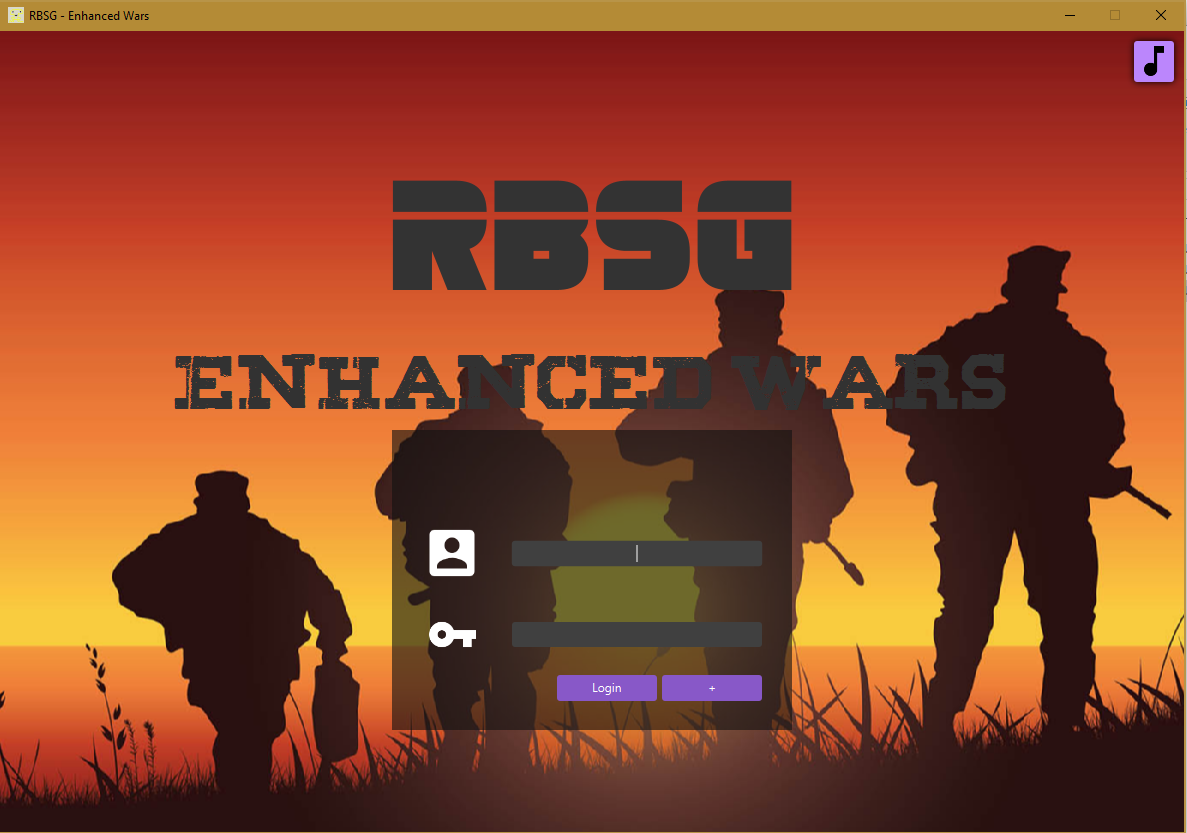
\includegraphics[width=0.8\textwidth]{Login_Release_One.PNG}
				\caption{Login Release \RN{1}}
				\label{Login_Release_One}
			\end{figure}
		\subsubsection{Lobby}
		Die Lobby zu Beginn des zweiten Releases wird in Abb. \ref{Lobby_Release_One} dargestellt. In der Lobby werden die Spielerlisten und Spiellisten angezeigt. Diese aktualisieren sich, wenn der Server eine entsprechende Nachricht sendet. Es ist m�glich �ber den \glqq Spiel erstellen\grqq-Knopf ein Spiel zu erstellen. �ber den \glqq Logout\grqq-Knopf kann ein Nutzer sich abmelden.
		\begin{figure}[H] 
			\centering
			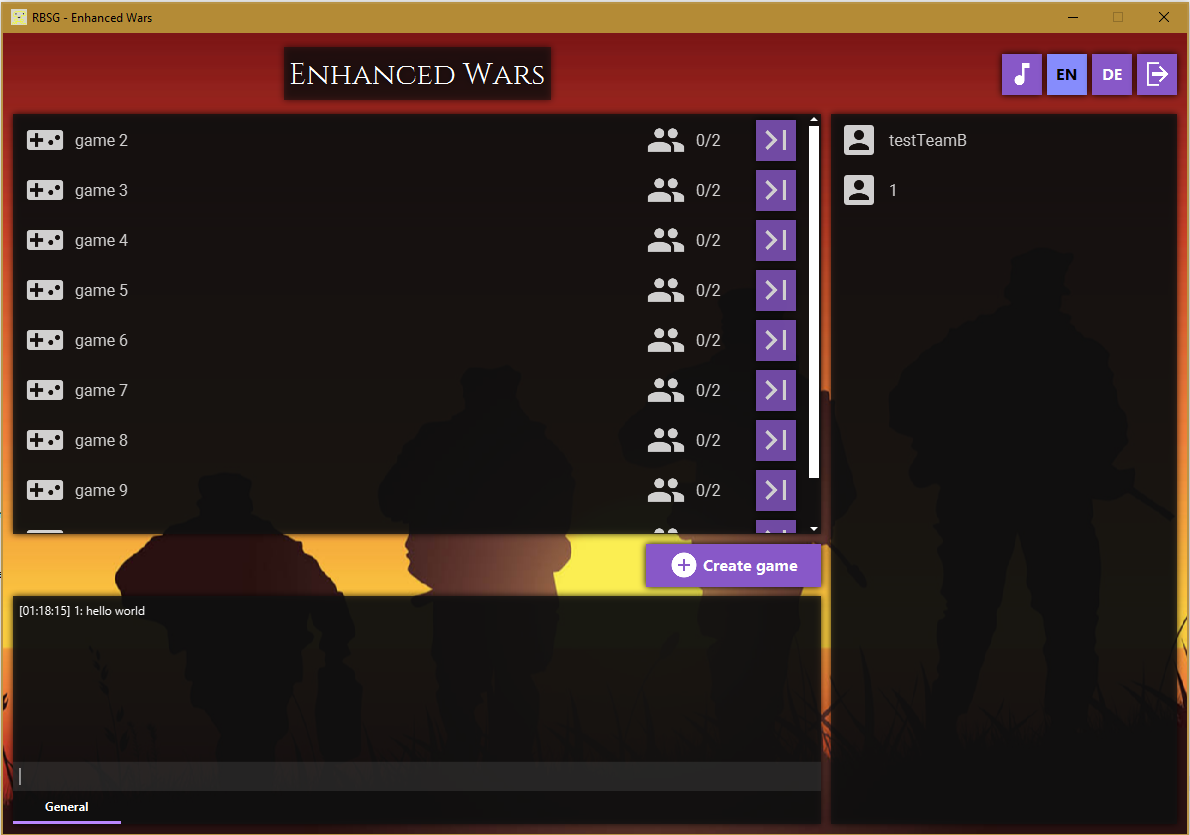
\includegraphics[width=0.8\textwidth]{Lobby_Release_One.PNG}
			\caption{Lobby Release \RN{1}}
			\label{Lobby_Release_One}
		\end{figure}
		\subsubsection{Spiel erstellen}
		Der in Abb. \ref{CreateGame_Release_One} dargestellte \glqq Spiel erstellen\grqq Dialog wird �ber den entsprechenden Button in der Lobby aufrufen. Im Spiel erstellen Fenster hat man die M�glichkeit, den Name des Spiels und die Anzahl der Spieler einzustellen.\footnote{2-Spieler und 4-Spieler} Das Spiel wird �ber den \glqq Erstellen\grqq-Button erzeugt und �ber den \glqq Abbrechen\grqq-Button kann man den Dialog wieder verlassen.
		\begin{figure}[H] 
			\centering
			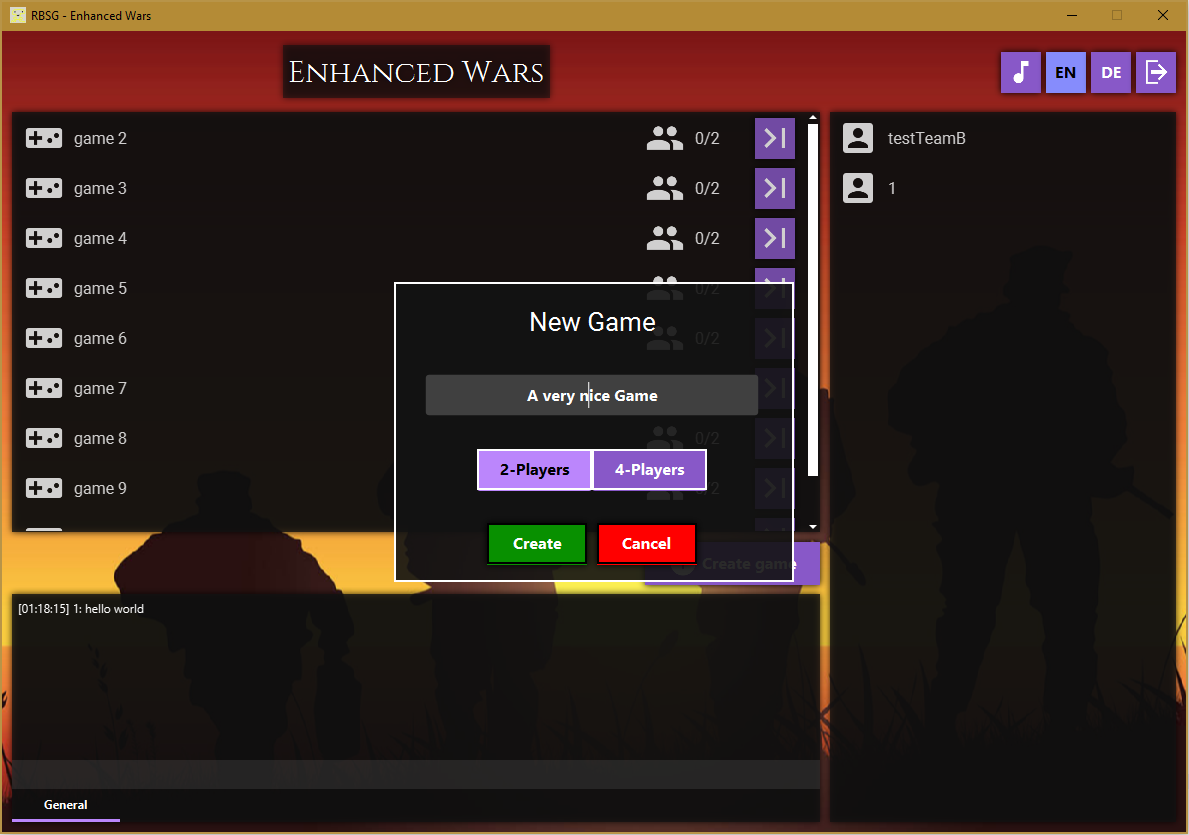
\includegraphics[width=0.8\textwidth]{CreateGame_Release_One.PNG}
			\caption{Spiel erstellen Release \RN{1}}
			\label{CreateGame_Release_One}
		\end{figure}
		\subsubsection{Spiel beitreten}
		�ber den Knopf in der Spielliste kann man einem Spiel, entsprechend dem Serverstand des ersten Releases, beitreten. Nachdem man einem Spiel beigetreten ist, wechselt die Szene zum Warteraum des Spiels. Der Warteraum eines Spiels zum Stand nach dem ersten Release wird in Abb. \ref{WaitingRoom_Release_One} dargestellt.
		 \begin{figure}[H] 
		 	\centering
		 	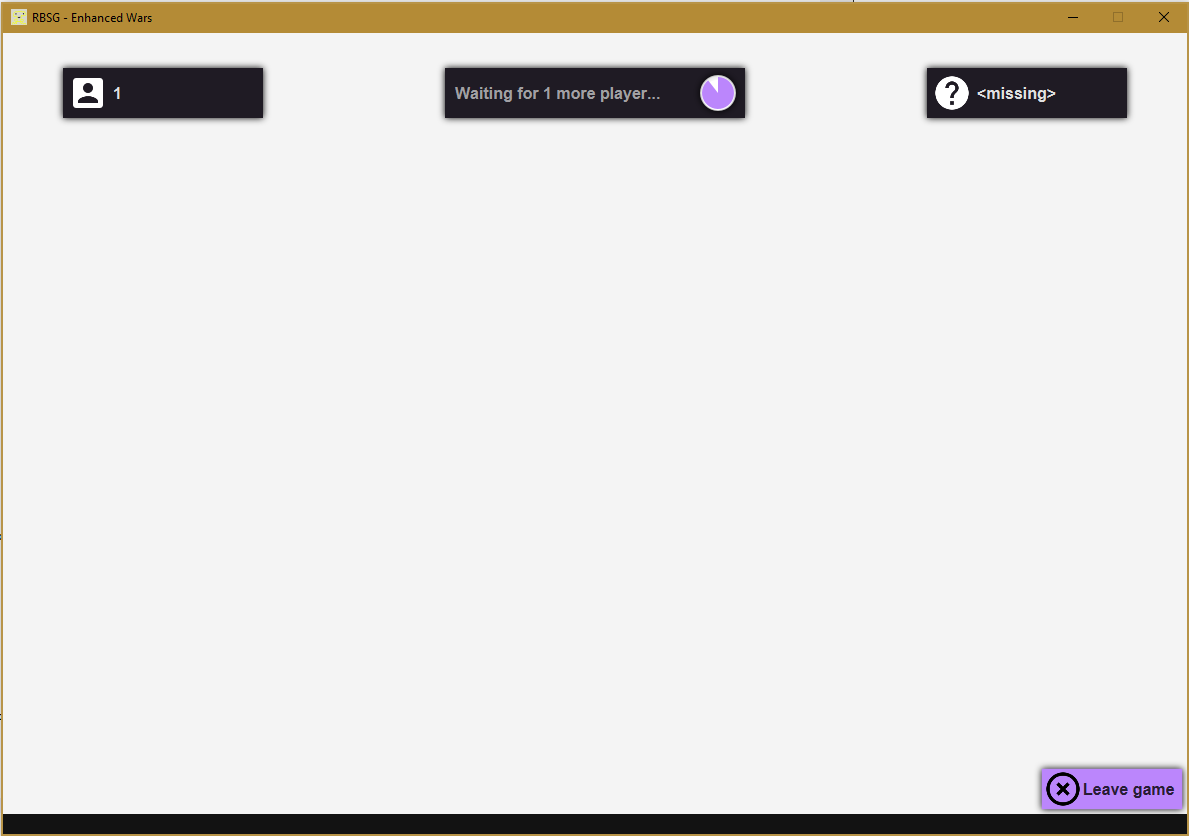
\includegraphics[width=0.8\textwidth]{WaitingRoom_Release_One.PNG}
		 	\caption{Warteraum eines Spiels Release \RN{1}}
		 	\label{WaitingRoom_Release_One}
		 \end{figure}
	 	\subsubsection{Lobby Chat}
	 	Die Lobby verf�gte bereits �ber einen Chat. Mit diesem ist es m�glich Nachrichten in den General-Chat und in Private-Chats zu versenden.
	 	\subsubsection{Umgesetzte Optionale Features}
	 	Im ersten Release wurden bereits folgende optionale Features umgesetzt:
	 	\begin{itemize}
	 		\item Internationalisierung, diese kann �ber Buttons, siehe Abb. \ref{Internationalisierung_Release_One}, in der Lobby eingestellt werden 
	 		\item Musik, diese kann �ber einen Button (Abb. \ref{Musik_Release_One}) an- und ausgestellt werden 
	 		\item Ein Dark-Theme 
	 		\item �ber den Chat-Befehl \glqq \textbackslash chuckMe\grqq werden Chuck Norris Zitate an den Chat gesendet
	 	\end{itemize}
 		Die Testabdeckung (C0) lag bei $\sim$ 80 Prozent, womit die Anforderung f�r das zweite Release bereits grundlegend erf�llt ist. Das Ziel f�r das zweite Release war es, die H�he der Testabdeckung aufrechtzuerhalten und weiter auszubauen.
 		\begin{figure}[H] 
 			\centering
 			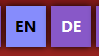
\includegraphics[width=0.2\textwidth]{Internationalisierung_Release_One.PNG}
 			\caption{Button f�r die Internationalisierung Release \RN{1}}
 			\label{Internationalisierung_Release_One}
 		\end{figure}
 		\begin{figure}[H] 
 			\centering
 			
\includegraphics[width=0.1\textwidth]{Musik_Release_One.PNG}
 			\caption{Button f�r Musik Release \RN{1}}
 			\label{Musik_Release_One}
 		\end{figure}
 		
	\subsection{Mockups}
		F�r das Kundentreffen am 27.05.2019 wurden Mockups f�r den Armenkonfigurator, im folgenden als ArmyBuilder bezeichnet, und dem Waiting Room vorbereitet. Eine Besonderheit der erstellten Mockups ist, dass diese den Stil der bisherigen Applikation �bernehmen. Damit soll dem Kunden ein Eindruck vom sp�teren Produktes vermittelt werden. Nach der Ver�ffentlichung der zweiten Serverdokumentation, wurden die Mockups daraufhin angepasst. Insbesondere das  Lobby Mockup wurde erweitert.
		\subsubsection{ArmyBuilder}
			Der ArmyBuilder besteht insgesamt aus 3 Komponenten:
			\begin{enumerate}
				\item der Einheitenauswahl
				\item der Armeeauswahl
				\item der Armee�bersicht
			\end{enumerate}
		Das Kernst�ck des ArmyBuilders sind die konfigurierbaren Armeen. Auf der rechte Seite werden in einer Liste sieben Armeen, in Form ihrer Icons angezeigt. Mit einem Linksklick auf ein Armee Icon, wird die entsprechende Armee ausgew�hlt und die Detailinformationen dieser Armee werden angezeigt. Zu den Inforamtionen geh�ren der Armeename sowie die Einheiten, aus denen die Armee besteht. In der Einheitenauswahl werden alle verf�gbaren Einheitentypen aufgelistet. Ist eine Einheit ausgew�hlt, wird eine Detailansicht zu dieser Einheit angezeigt, mit Informationen, wie Attributen und einem Bild. �ber den \glqq +\grqq Button ist es m�glich eine Einheit der ausgew�hlten Armee hinzuzuf�gen. Die Einheit wird anschlie�en der Armee�bersicht hinzugef�gt und entsprechende Informationen werden aktualisiert. Der Nutzer kann in der Armee�bersicht ebenfalls Einheiten ausw�hlen. Der ausgew�hlte Einheitentyp wird dann in der Detailansicht angezeigt. �ber den \glqq -\grqq kann die Einheit dann wieder aus der Armee entfernt werden. �ber den \glqq Speichern\grqq-Button k�nnen die Armee auf dem Server und lokal gespeichert werden. Mit dem \glqq Info\grqq-Button hat der Nutzer die M�glichkeit sich die angezeigten Symbole erl�utern zu lassen. Dazu wurde eine entsprechendes Mockup erstellt, dieses ist in \Abb{InfoView} zu sehen.\\ \\ F�r den ArmyBuilder wurden zwei Designs entworfen, siehe \Abb{ArmyBuilder_Design_One} und \Abb{ArmyBuilder_Design_Two}. Das Team hat sich auf das zweite Design geeinigt. 
		\begin{figure}[H] 
			\centering
			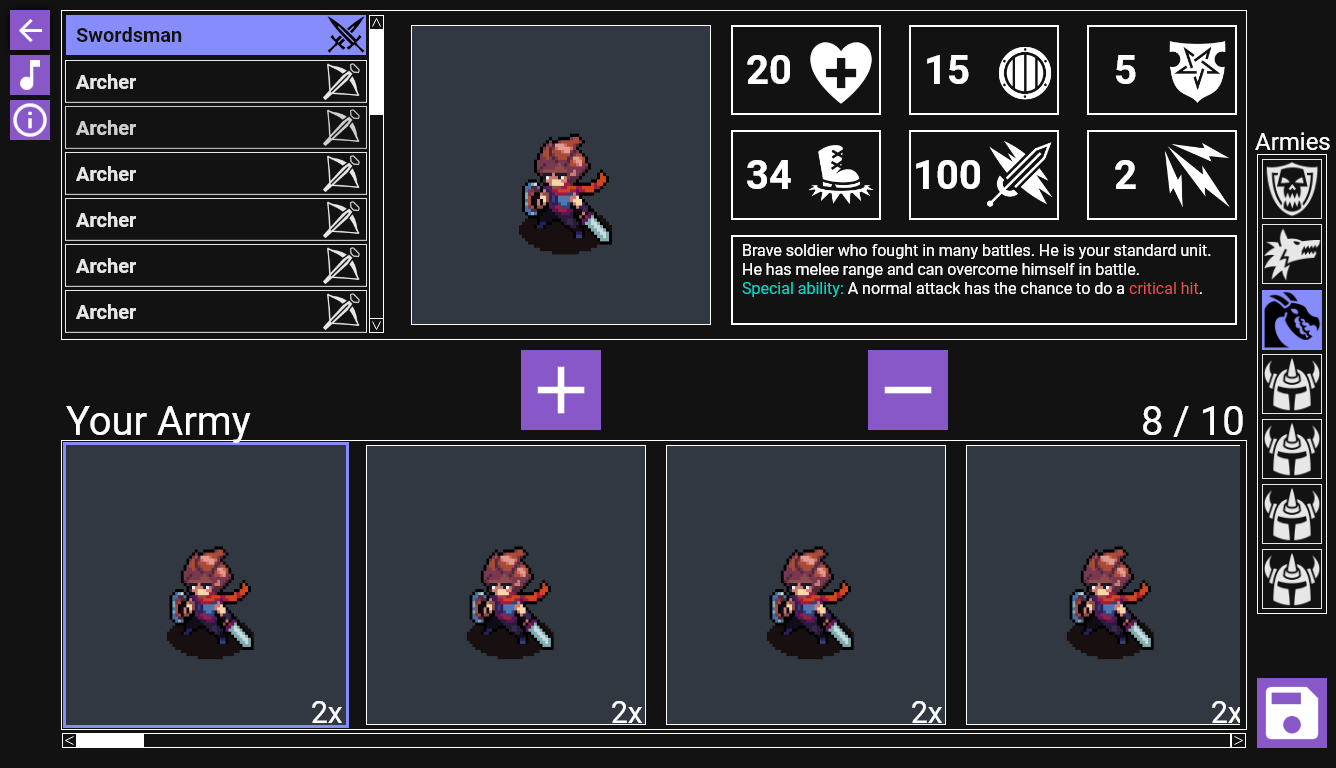
\includegraphics[width=0.8\textwidth]{ArmyBuilder_Design_One.png}
			\caption{Mockup ArmyBuilder Design \RN{1} }
			\label{ArmyBuilder_Design_One}
		\end{figure}
		\begin{figure}[H] 
			\centering
			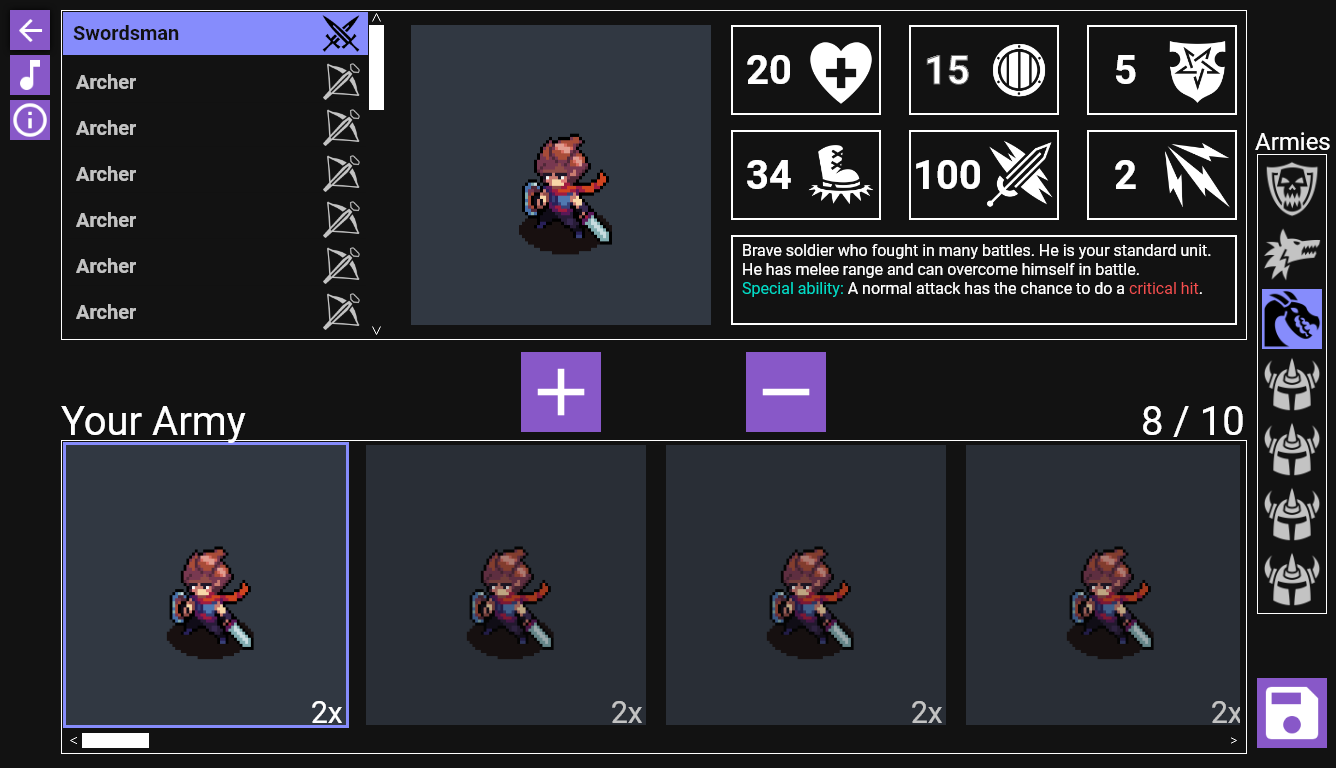
\includegraphics[width=0.8\textwidth]{ArmyBuilder_Design_Two.png}
			\caption{Mockup ArmyBuilder Design \RN{2} }
			\label{ArmyBuilder_Design_Two}
		\end{figure}
		\begin{figure}[H] 
			\centering
			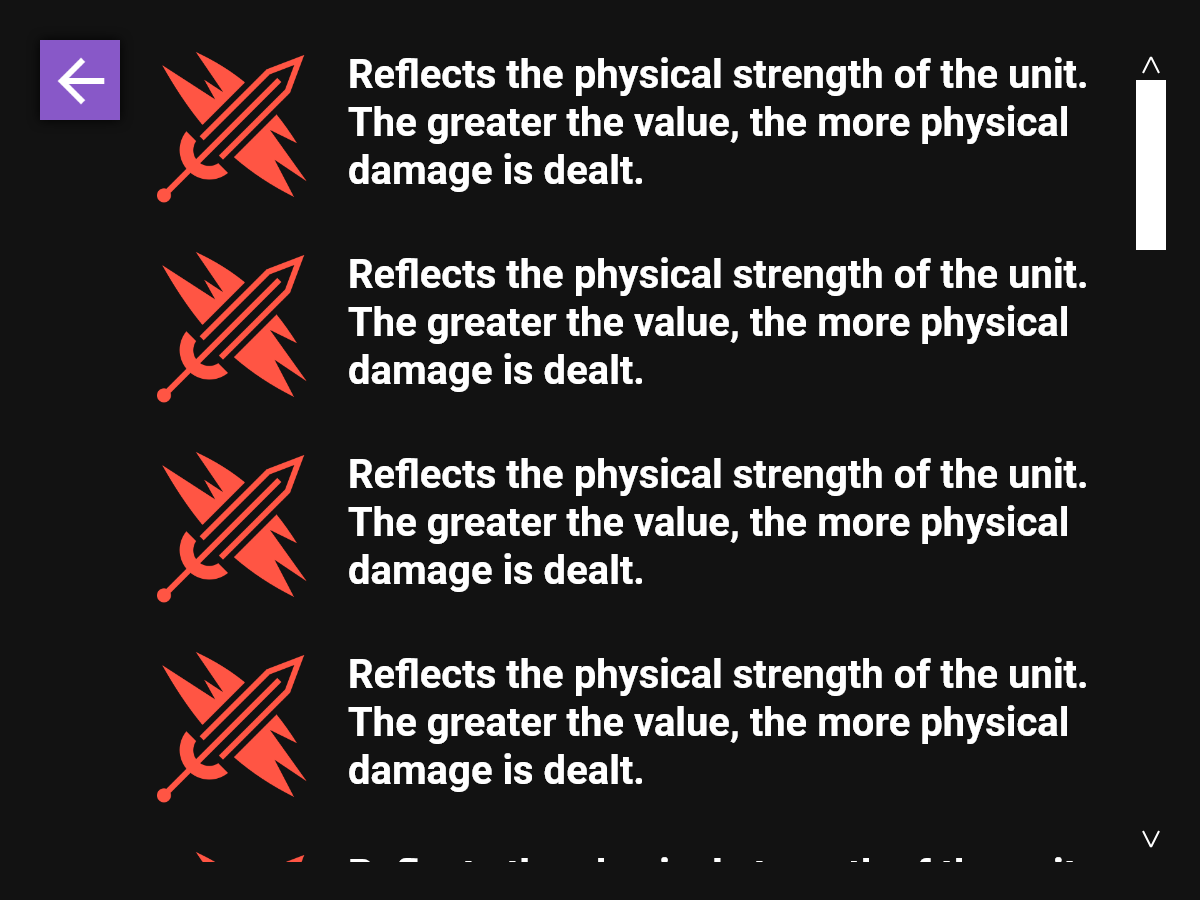
\includegraphics[width=0.5\textwidth]{InfoView.png}
			\caption{Mockup Informationsanzeige \RN{2} }
			\label{InfoView}
		\end{figure}
		
		\ \\Im Kundentreffen wurde der Wunsch ge�u�ert, die Armee Icons ausw�hlen zu k�nnen. Daf�r wurde eine entsprechender Button zu der Liste der Armeeauswahl hinzugef�gt \Abb{ArmyBuilder_EditButton}. Durch Bet�tigen des Buttons wird ein Dialog (Abb. \ref{AmryEditor}) ge�ffnet, in dem das Icon sowie der Name der Armee bearbeitet werden kann. Eine Auswahl an Icons wird daf�r bereitgestellt.
		\begin{figure}[H] 
			\centering
			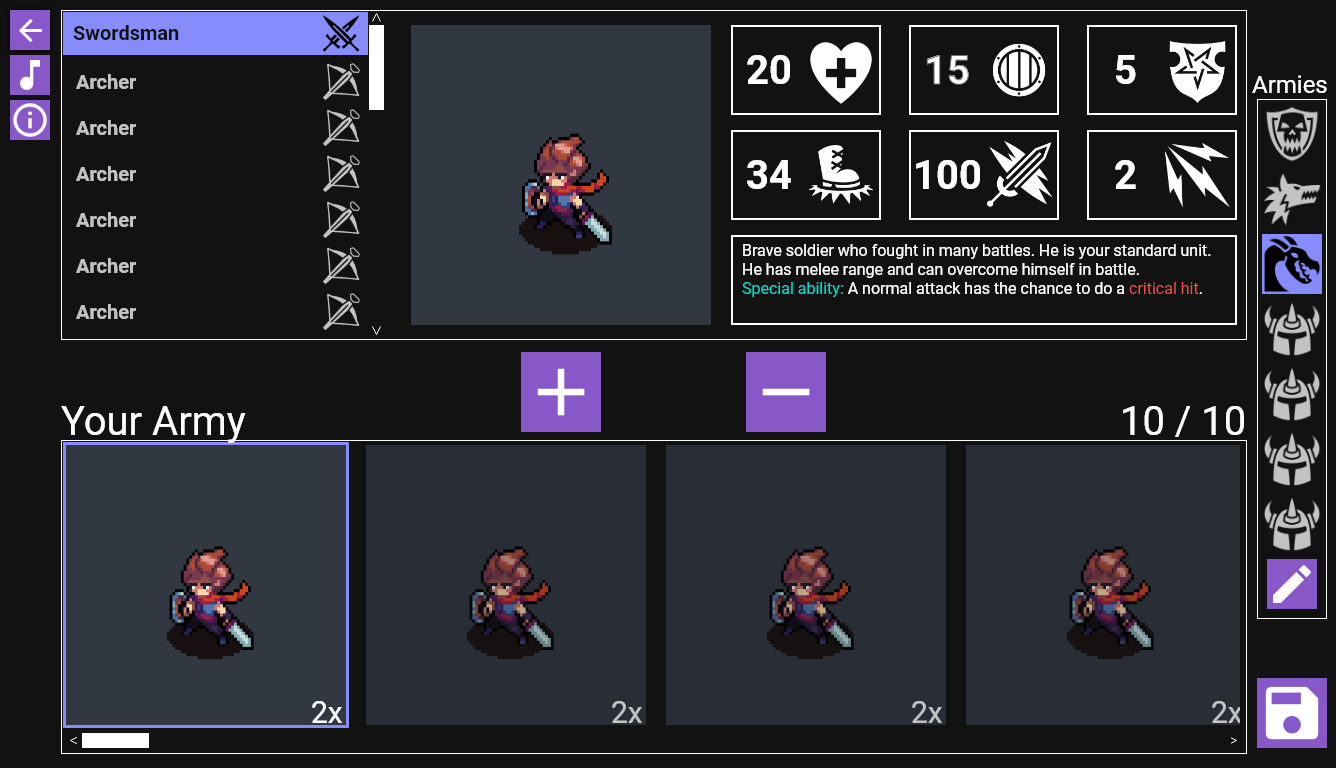
\includegraphics[width=0.8\textwidth]{ArmyBuilder_Save_Edit.png}
			\caption{Mockup ArmyBuilder mit \glqq Bearbeitungs\grqq-Button f�r Armeeicons}
			\label{ArmyBuilder_EditButton}
		\end{figure}
		\begin{figure}[H] 
			\centering
			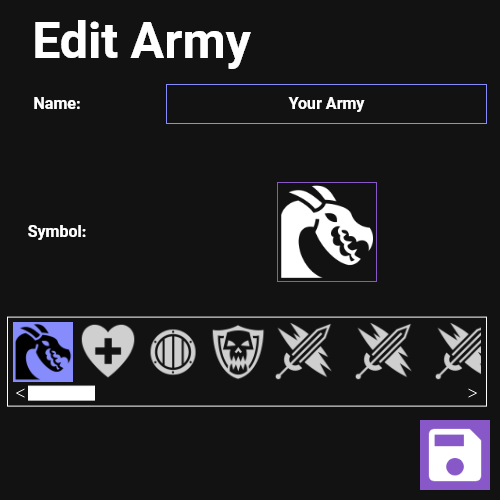
\includegraphics[width=0.5\textwidth]{ArmyEditor.png}
			\caption{Mockup Armee Icon Bearbeitung}
			\label{AmryEditor}
		\end{figure}
		In den Mockups werden unterschiedliche Zust�nde des ArmyBuilders dargestellt:
		\begin{itemize}
			\item Eine Armee ist leer. Es k�nnen Einheiten hinzugef�gt werden \Abb{ArmyBuilder_AddUnits}.
			\item Es ist keine Einheit in der Einheitenauswahl ausgew�hlt. Es k�nnen keine Einheiten der Armee hinzugef�gt werden \Abb{ArmyBuilder_Select_Unit}. 
		\end{itemize}
		\begin{figure}[H] 
			\centering
			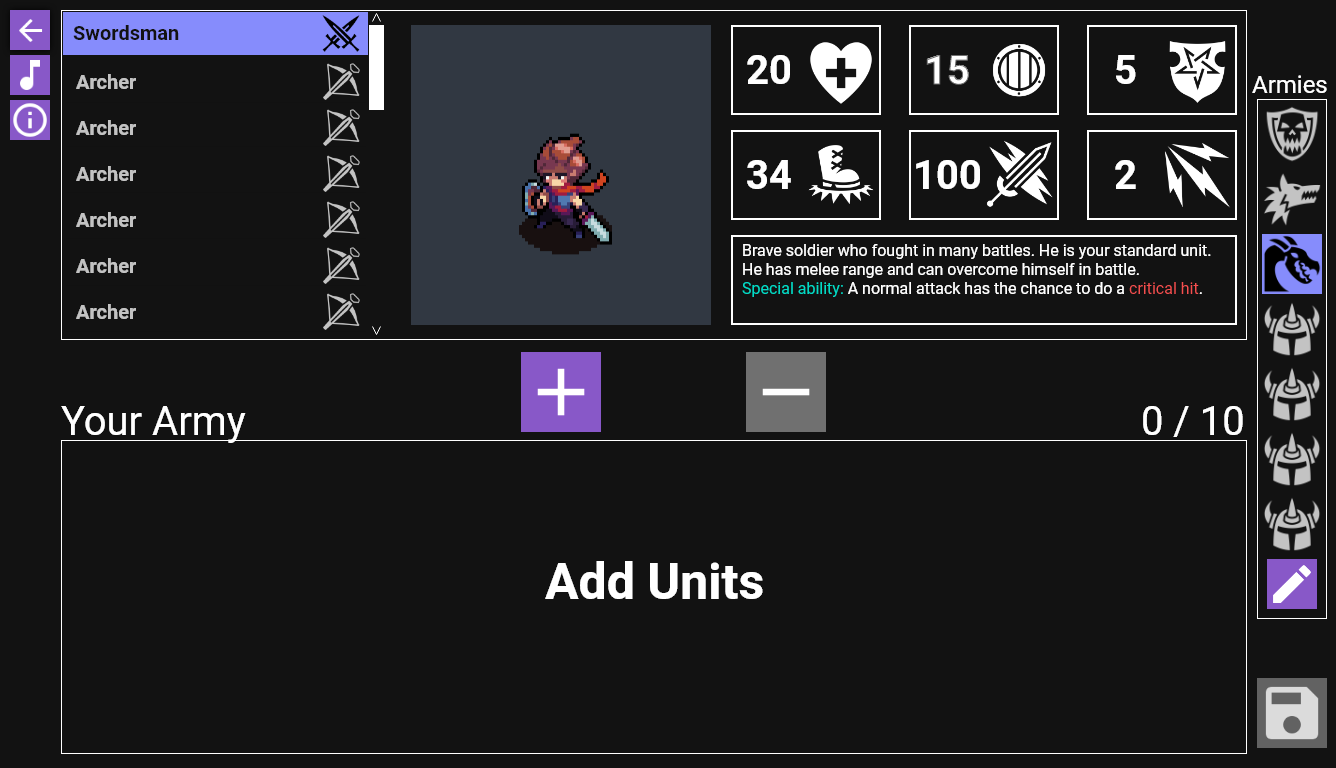
\includegraphics[width=0.5\textwidth]{Army_Builder_Add_Units.png}
			\caption{Mockup ArmyBuilder eine Armee enth�lt keine Einheiten}
			\label{ArmyBuilder_AddUnits}
		\end{figure}
		\begin{figure}[H] 
			\centering
			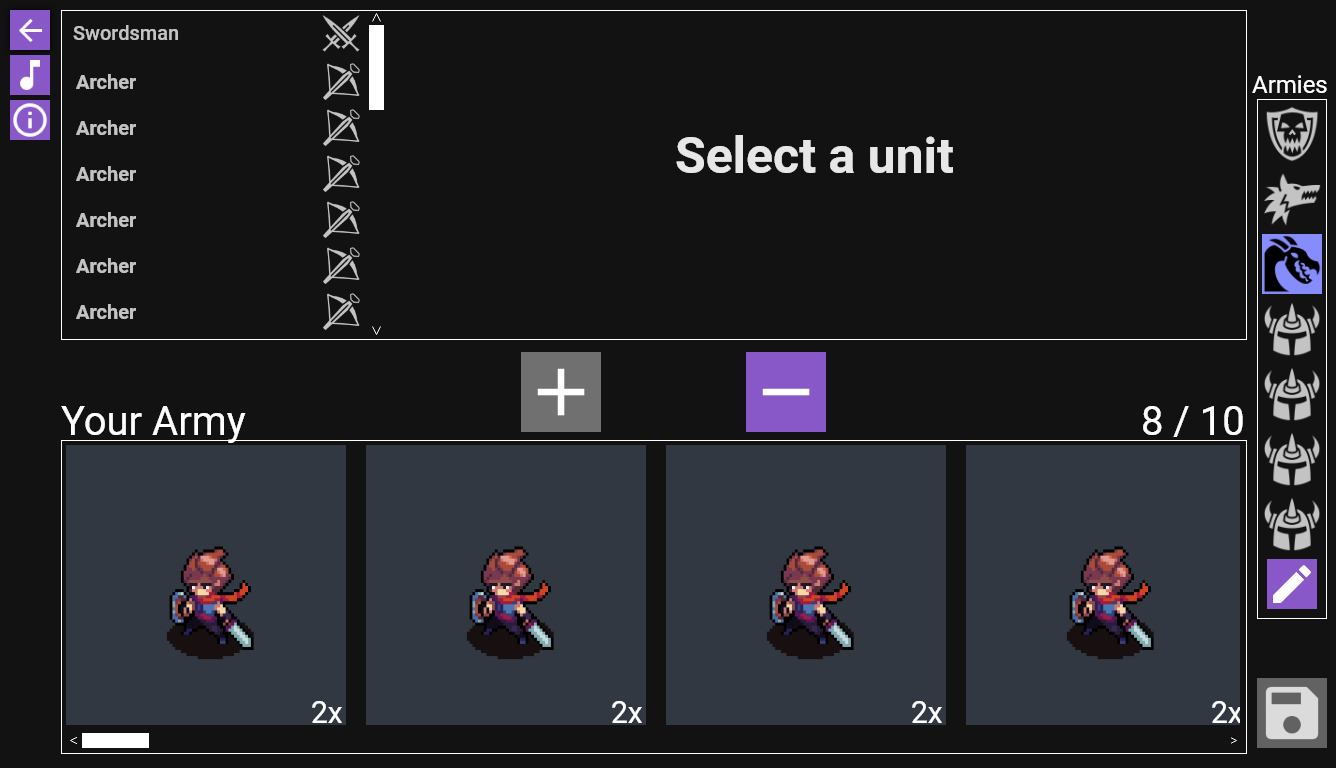
\includegraphics[width=0.5\textwidth]{ArmyBuilder_Select_Unit.png}
			\caption{Mockup ArmyBuilder es ist keine Einheit ausgew�hlt}
			\label{ArmyBuilder_Select_Unit}
		\end{figure}
		\begin{figure}[H] 
			\centering
			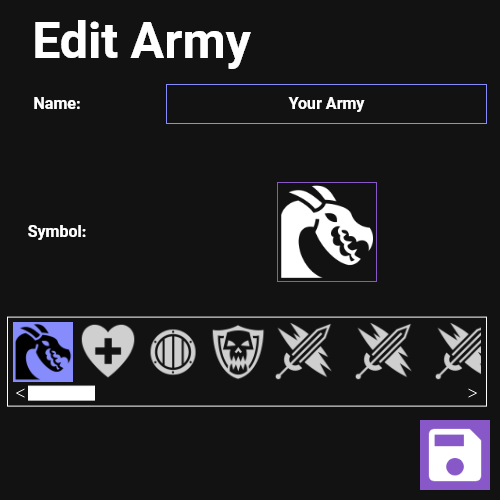
\includegraphics[width=0.5\textwidth]{ArmyEditor.png}
			\caption{Mockup ArmyBuilder Design}
			\label{AmryEditor}
		\end{figure}
		
		\subsection{Lobby}
		Um einem Spiel beitreten zu k�nnen muss ein Spieler �ber eine g�ltige Armee-ID verf�gen, d. h. eine g�ltige Armee ausgew�hlt haben. Dazu erweitern wir die Lobby um eine Armeeauswahl. Dies wird in \Abb{Lobby_with_Army} dargestellt. Wie im ArmyBuilder werden die Armeen �ber die zugeh�rigen Icons dargestellt. Ist eine Armee nicht ausw�hlbar, so wird diese grau hinterlegt dargestellt. 
		\begin{figure}[H] 
			\centering
			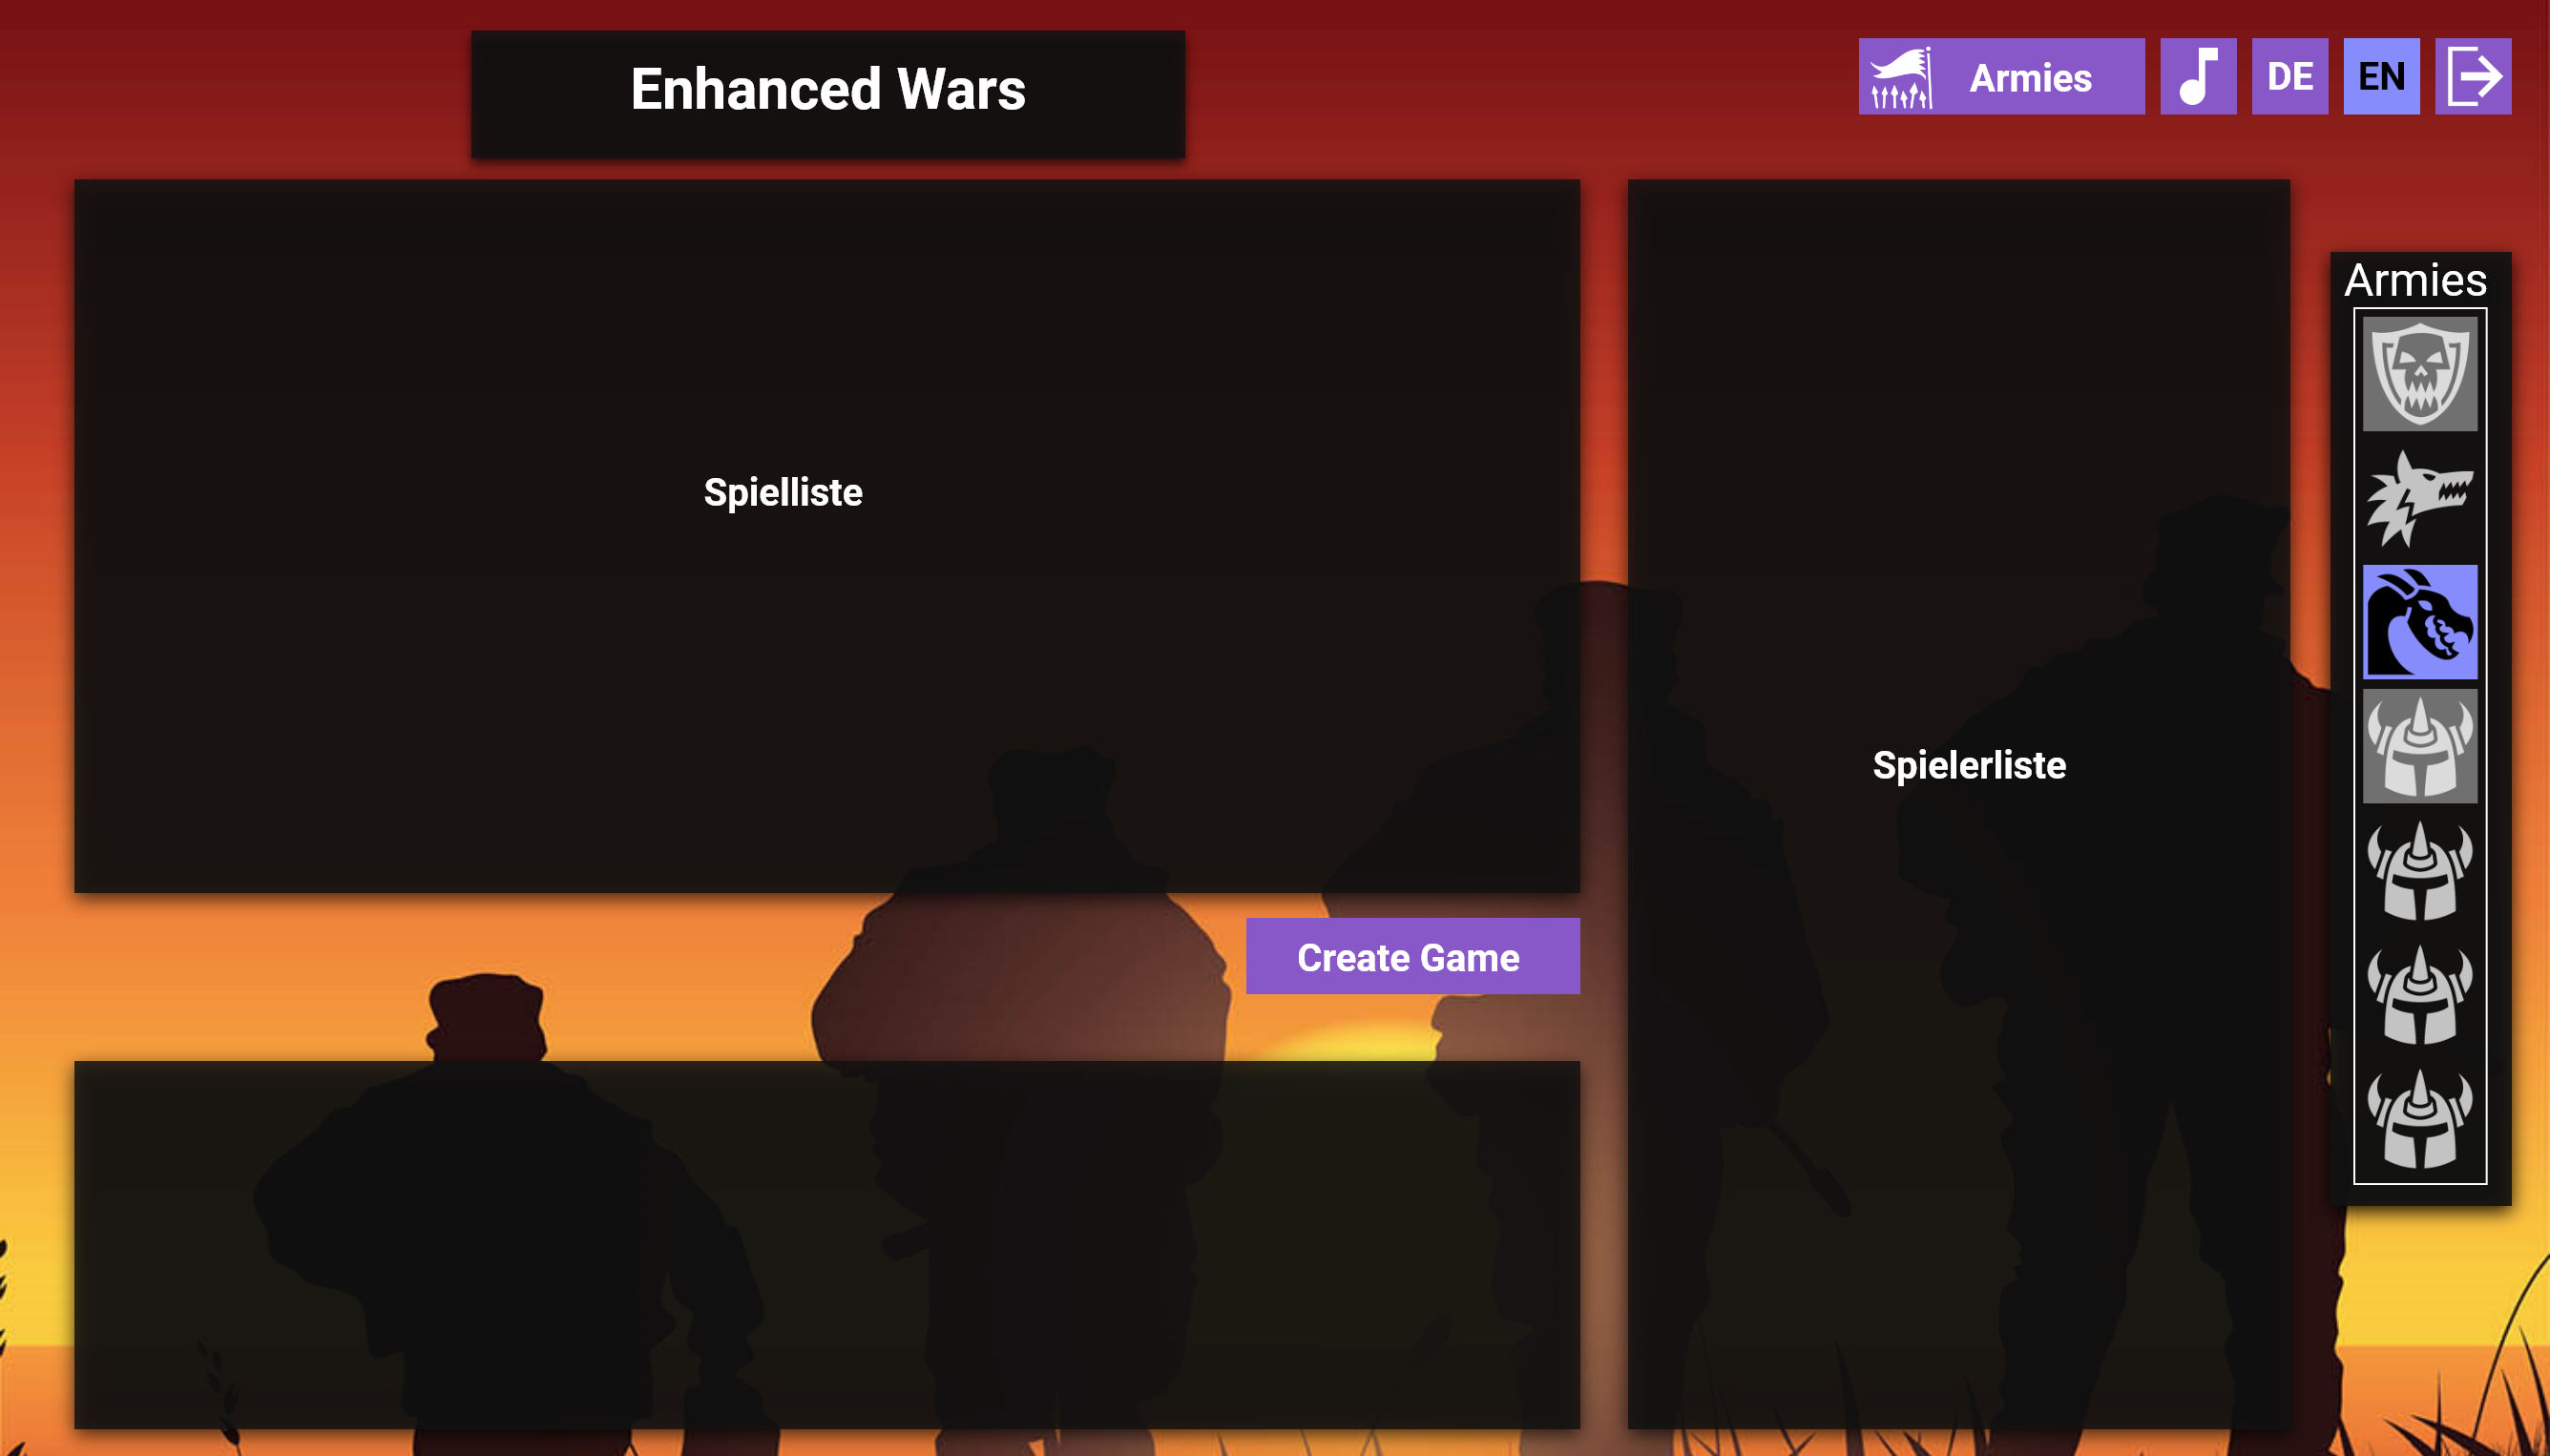
\includegraphics[width=0.8\textwidth]{Lobby_mit_Army_Button_und_Armeeliste.png}
			\caption{Mockup Lobby mit Armeeauswahl und Armee-Button}
			\label{Lobby_with_Army}
		\end{figure}
		
		\subsubsection{Waiting Room}
		F�r den Waiting Room waren aus dem vorherigen Release Mockups und eine anf�ngliche Realisierung vorhanden. Diese haben wir aufgegriffen und erweitert. Der Waiting Room besteht aus den Komponenten:
		\begin{itemize}
			\item dem Game Chat
			\item der Anzeige der Mitspieler
			\item der Anzeige des Spielfelds
			\item der Anzeige der gew�hlten Armee
		\end{itemize}
		Dieser ist auf \Abb{WaitingRoomWithArmy}
		\paragraph{Game Chat}
		�ber den Game Chat ist es m�glich mit den Mitspielern zu chatten. Es gibt einen Allgemeinen Chat und es sind Private Chats mit den anderen Spielern m�glich.
		\paragraph{Anzeige der Mitspieler}
		Jeder Spieler, der einem Spiel beigetreten ist, wird durch eine \glqq Spielerkarte \grqq dargestellt. In diesem wird der Name des Spielers und ein Spieler-Icon angezeigt. F�r jeden freien Platz wird ein Status sowie eine Warteanimation angezeigt.  
		\paragraph{Anzeige des Spielfelds}
		Eine Vorschau des Spielfeld wird in der Mitte des Waiting Rooms angezeigt. Es handelt sich hierbei um ein optionales Feature. !Das Spielfeld ist bereits auf dem Mockup enthalten, damit sich die Entwickler die Oberfl�che besser darstellen k�nnen und entsprechend vorbereiten k�nnen.!
		\paragraph{Anzeige der gew�hlten Armee}
		Die f�r das Spiel ausgew�hlte Armee soll auf der rechten Seite des Waiting Rooms angezeigt werden
		
		\begin{figure}[H] 
			\centering
			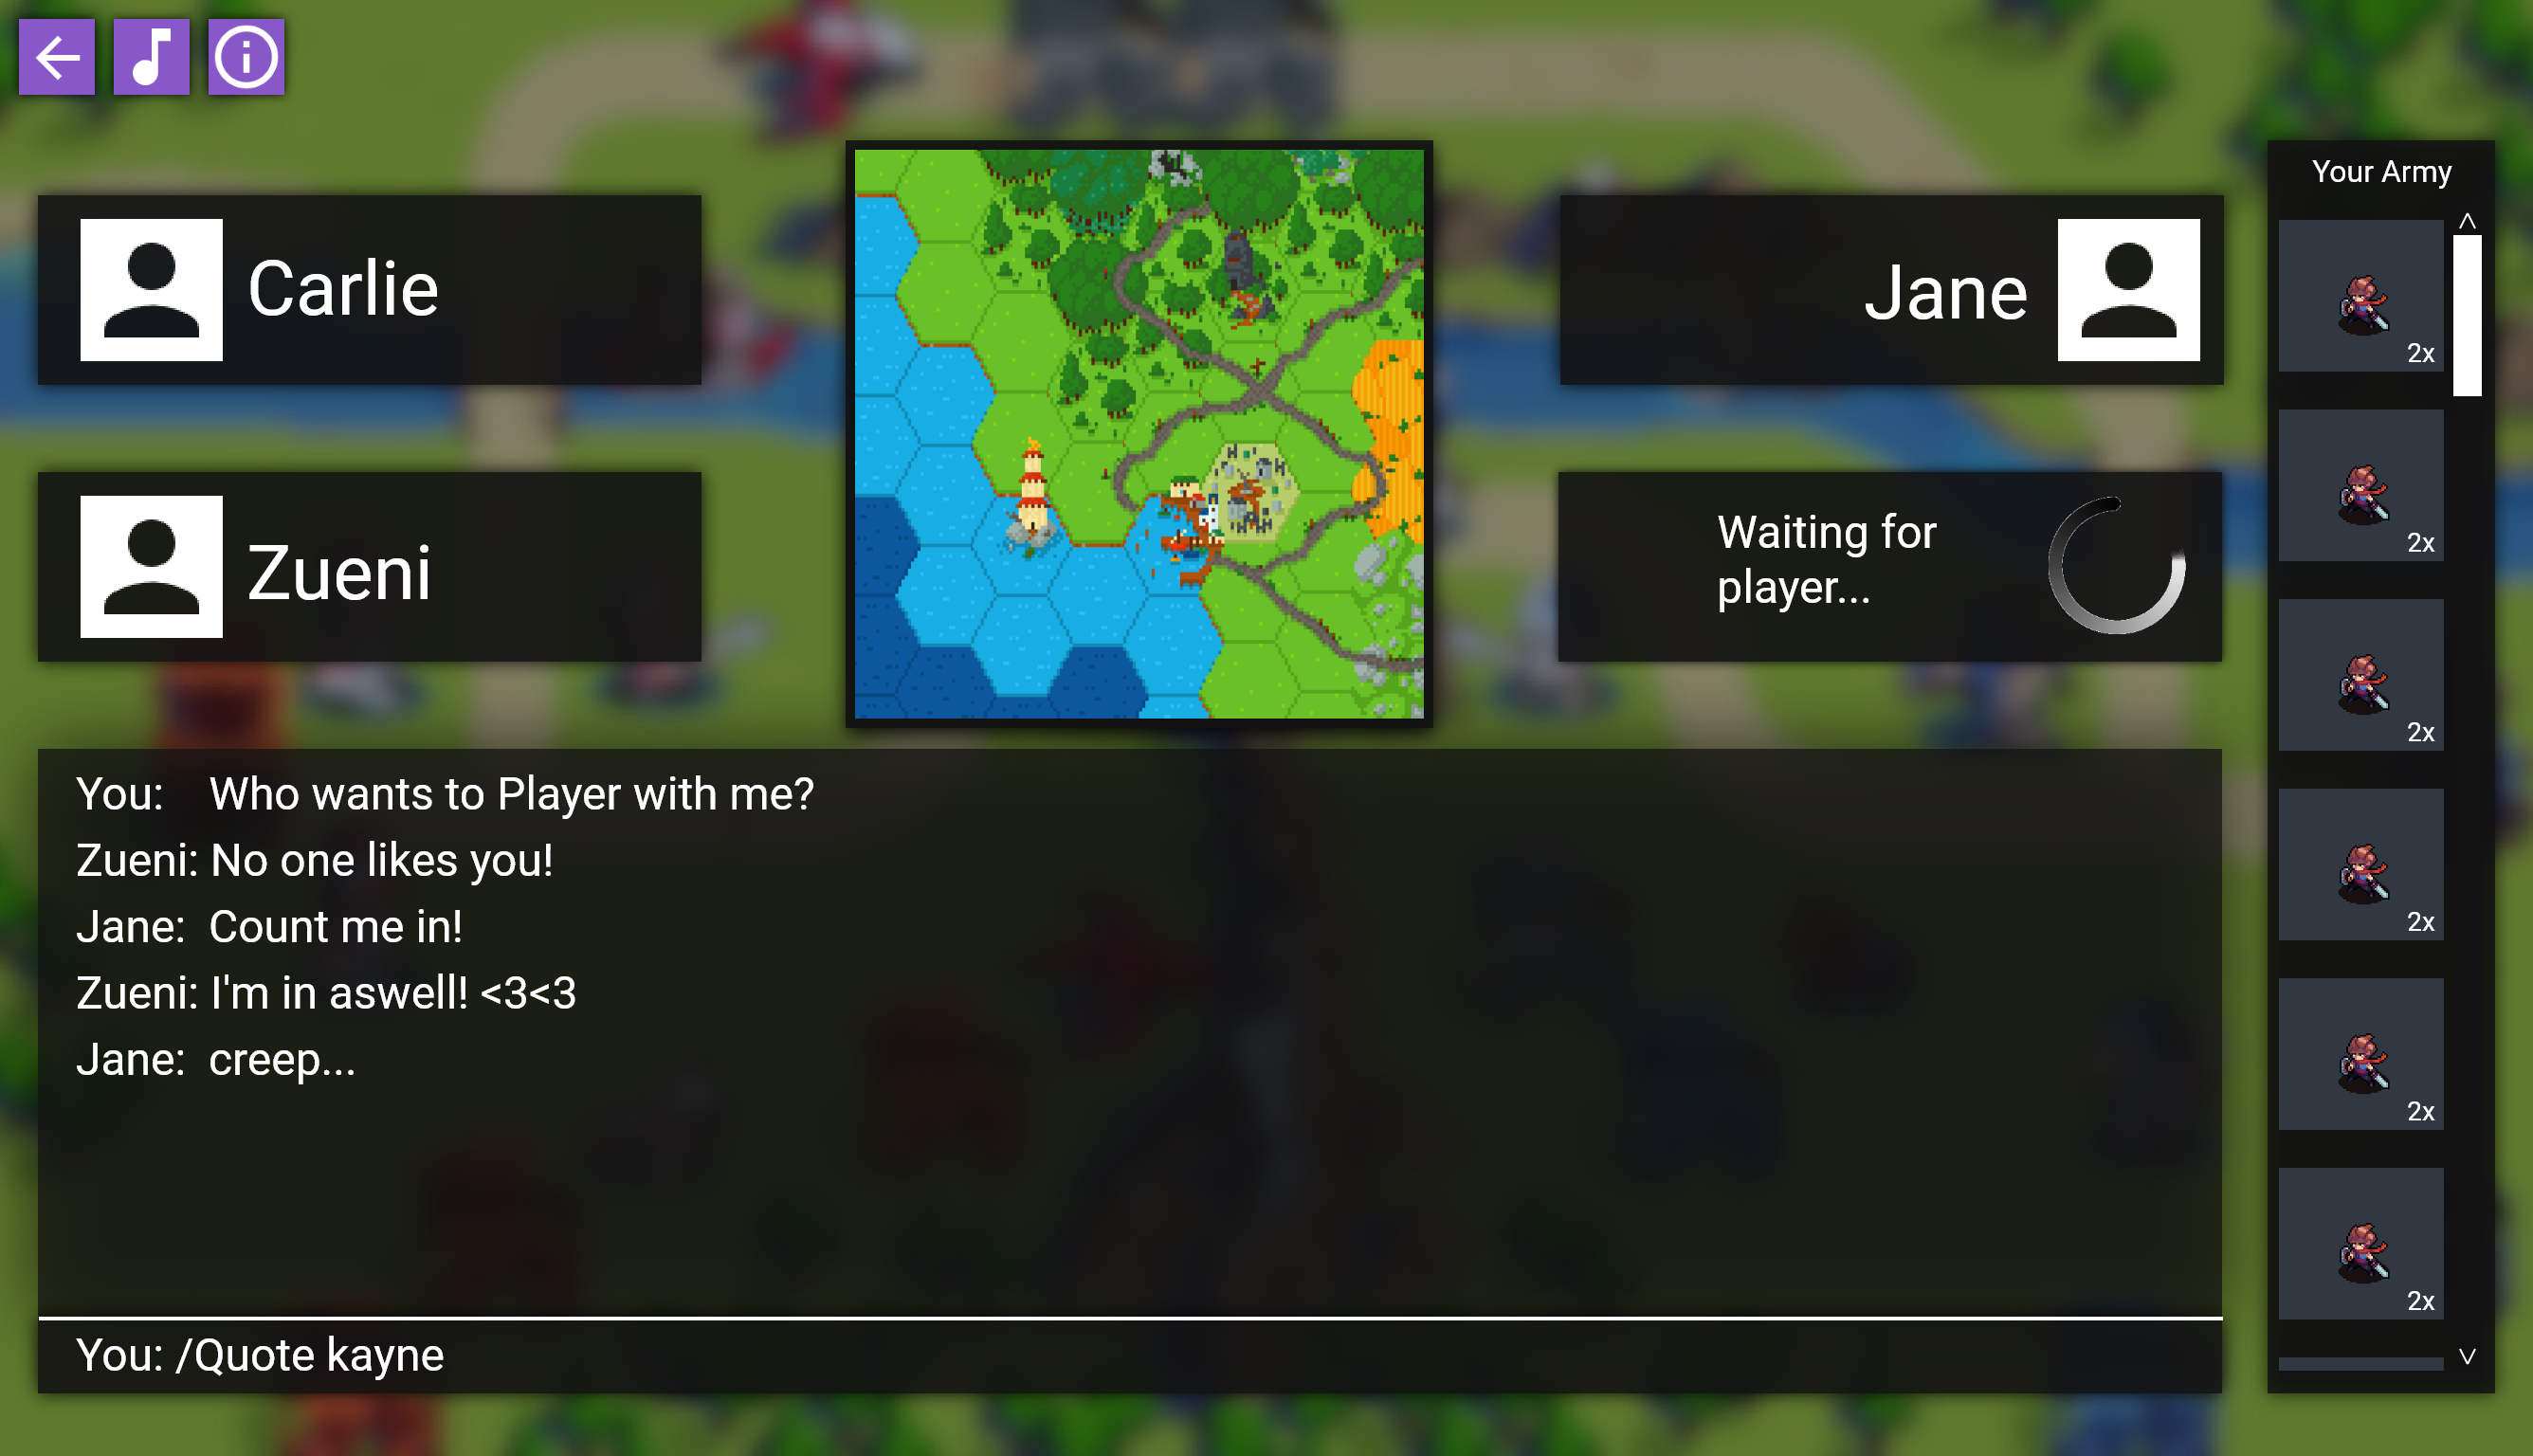
\includegraphics[width=0.8\textwidth]{Waiting_Room_Game_mit_ArmyView.png}
			\caption{Mockup Waiting Room mit Armeeanzeige}
			\label{WaitingRoomWithArmy}
		\end{figure}
	
		\paragraph{Mockups mit m�glichen Zusatzfeatures}
		Ein m�gliches Zusatzfeature ist ein Minispiel im Waiting Room. Ein Mockup ist auf \Abb{WaitingRoomWithMiniGame} zu sehen.
		
		\begin{figure}[H] 
			\centering
			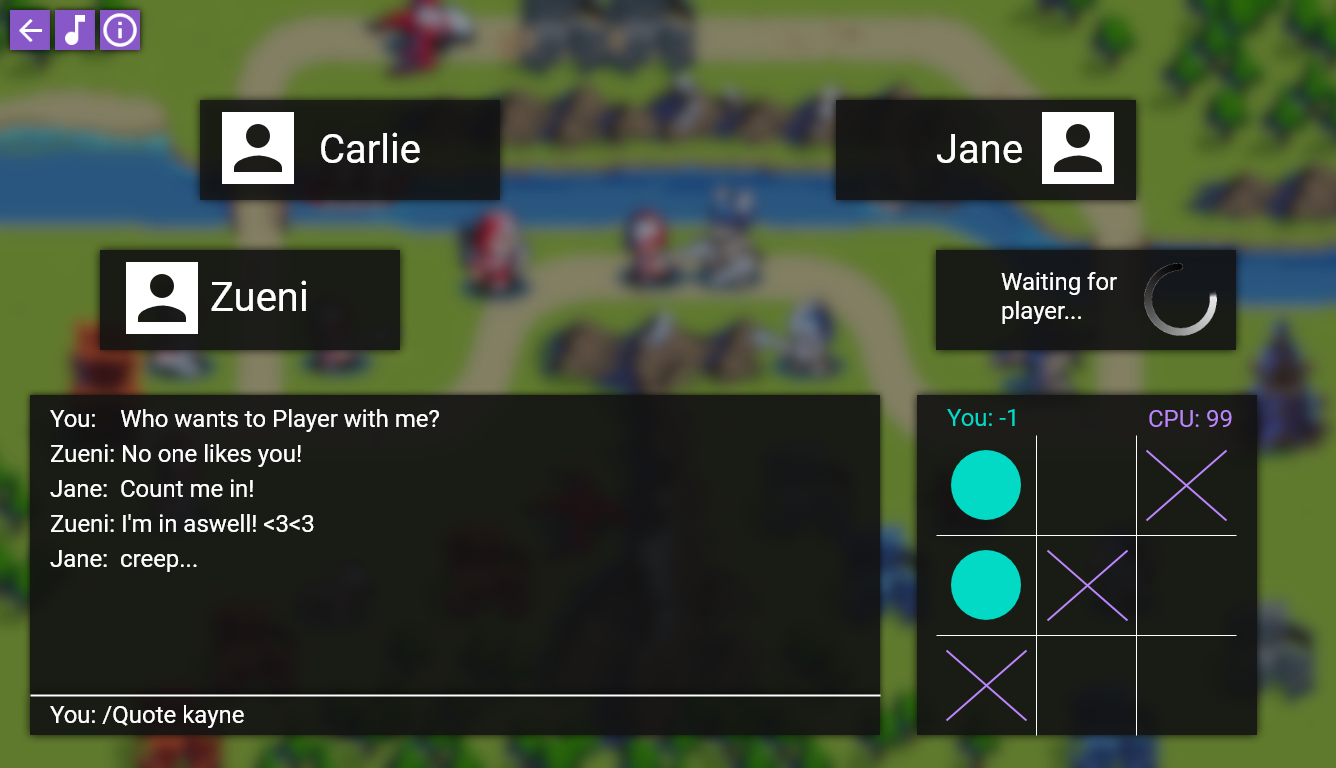
\includegraphics[width=0.8\textwidth]{Waiting_Room_Game_With_TTT.png}
			\caption{Mockup Waiting Room mit Minispiel}
			\label{WaitingRoomWithMiniGame}
		\end{figure}
	
		\paragraph{Nicht umsetzbare Mockups}
		Es wurde weitere Mockups erstellt. Diese enthalten Funktionalit�ten, die aufgrund der derzeitigen Server Implementierung nicht m�glich ist.\footnote{19.06.2019}
		
			\begin{figure}[H] 
				\centering
				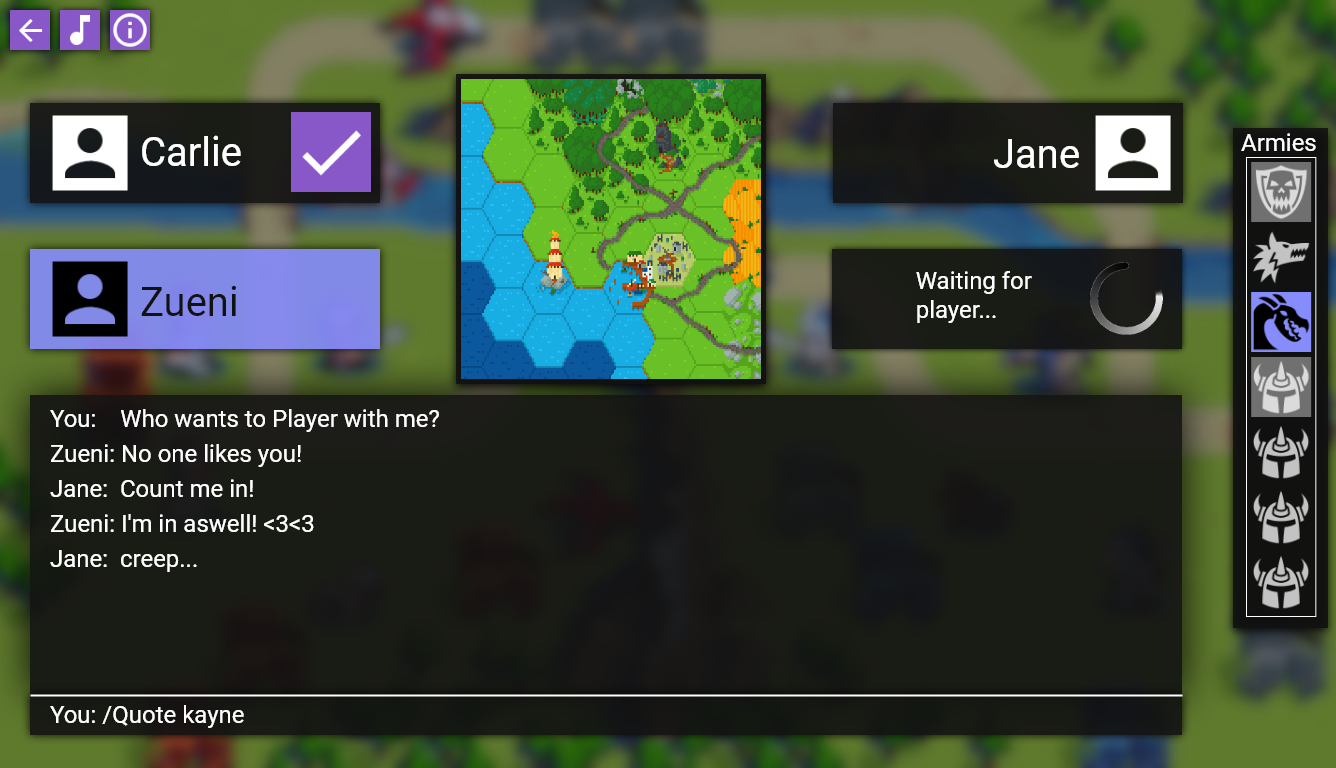
\includegraphics[width=0.8\textwidth]{Waiting_Room_Game_Mit_Map_Ready_Button.png}
				\caption{Mockup Waiting Room mit \glqq Ready\grqq-Button}
				\label{WaitingRoomWithReadyButton}
			\end{figure}
			\begin{figure}[H] 
				\centering
				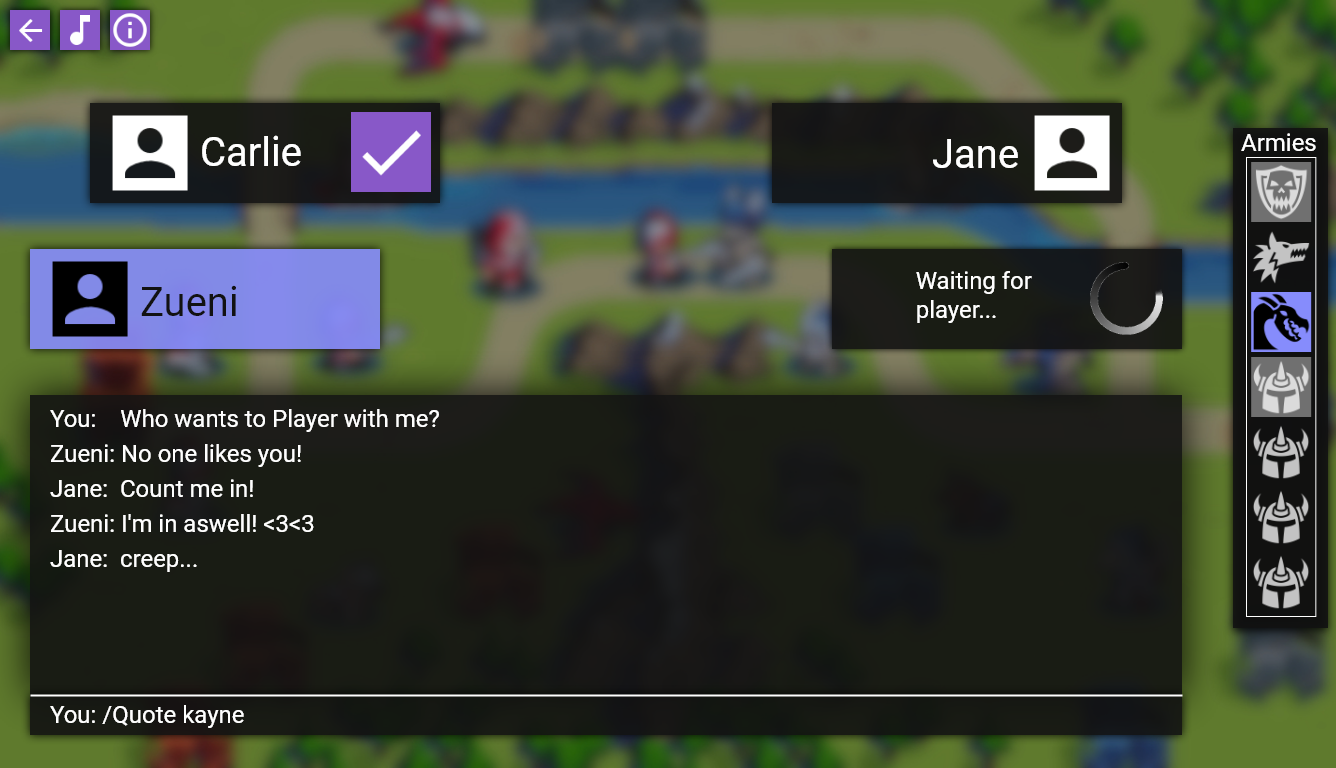
\includegraphics[width=0.8\textwidth]{Waitin_Room_Game_Ohne_Map.png}
				\caption{Mockup Waiting Room ohne Vorschaukarte und mit Armeeauswahl}
				\label{WaitingRoomWithOutMapAndWithArmySelector}
			\end{figure}
			\begin{figure}[H] 
				\centering
				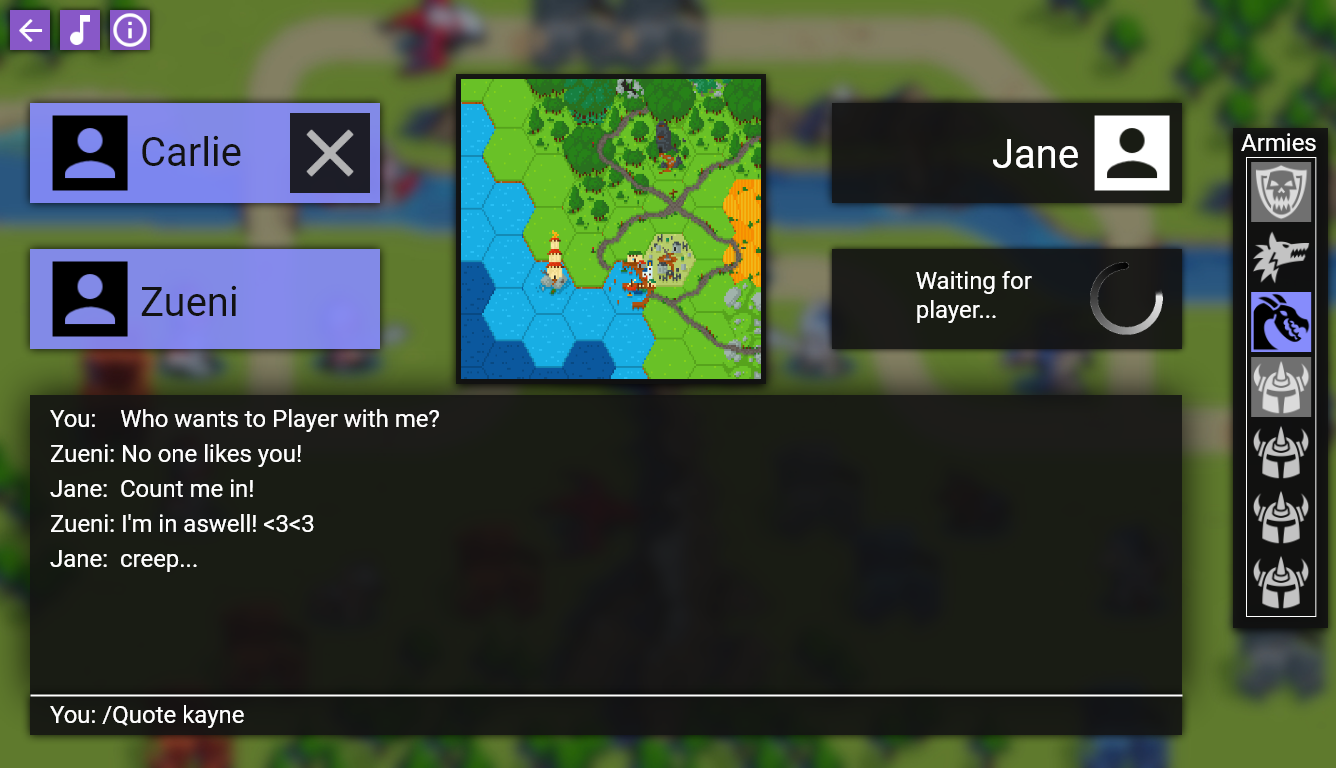
\includegraphics[width=0.8\textwidth]{Waiting_Room_Game_Mit_Map_Not_Ready.png}
				\caption{Mockup Waiting Room mit Map und mit \glqq Not Ready\grqq-Button}
				\label{WaitingRoomWithMapAndWithNotReayButton}
			\end{figure}
		
	\subsection{Domain Stories}
		Die Domoain Stories wurden erstellt, um dem Kunden eine m�gliche technische Realisierung der Anforderungen an dieses Release vorzustellen. Da zum Zeitpunkt der Kundenpr�sentation, die Serverdokumentation noch nicht bekannt war, sind die Domain Stories zum Teil unvollst�ndig oder allgemein gehalten. Die tats�chlich Umsetzung weicht vom Inhalt der Domain Stories ab.
	
		Die Domain Stories wurden erstellt, um dem Kunden eine m�gliche technische Realisierung der Anforderungen an dieses Release vorzustellen. Da zum Zeitpunkt der Kundenpr�sentation, die Serverdokumentation noch nicht bekannt war, sind die Domain Stories zum Teil unvollst�ndig oder allgemein gehalten. Die tats�chlich Umsetzung weicht vom Inhalt der Domain Stories ab.
		\subsubsection{Ingame - Zur�ck in die Lobby}
		Entsprechend den Anforderungen muss es m�glich sein, aus dem Spiel zur�ck in die Lobby zu wechseln. In Abb. \ref{DomainStoryZurueckInDieLobby} wird dargestellt, dass durch das Bet�tigen des Leave game-Buttons ein Szenenwechsel zur Lobby durchgef�hrt wird (1). Zeitgleich werden Game Controller Klassen benachrichtigt (2) (Abb. \ref{DomainStoryZurueckController}). Diese senden dem Server �ber den Spielwebsocket die Nachricht vom Spielaustritt (3). Im Fall, dass der Spieler, der das Spiel verl�sst, der Ersteller dieses Spiels war, wird eine DELETE Anfrage mit der ID des Spiels gesendet (4), wie in Abb. \ref{DomainStoryZurueckDelete} zu sehen. Zudem wird der Spiel-Websocket geschlossen (4) [sic].
		\begin{figure}[H] 
			\centering
			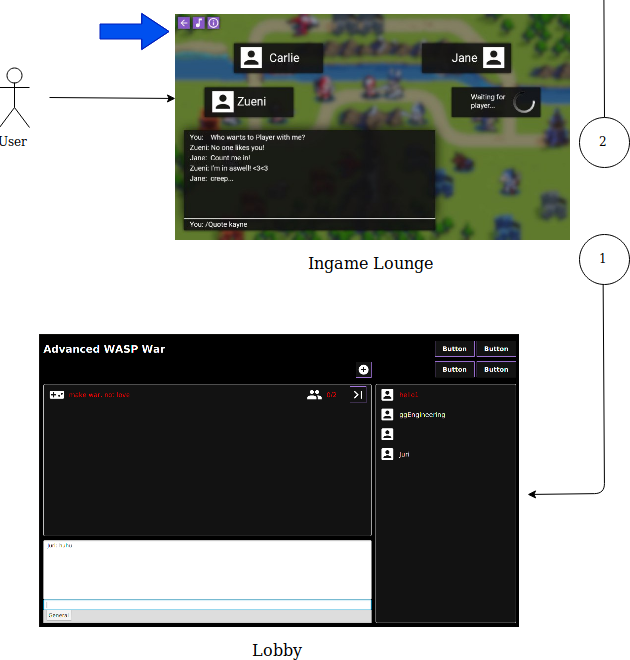
\includegraphics[width=0.7\textwidth]{BackToLobby1.png}
			\caption{Domain Story Zur�ck in die Lobby}
			\label{DomainStoryZurueckInDieLobby}
		\end{figure}
		\begin{figure}[H] 
			\centering
			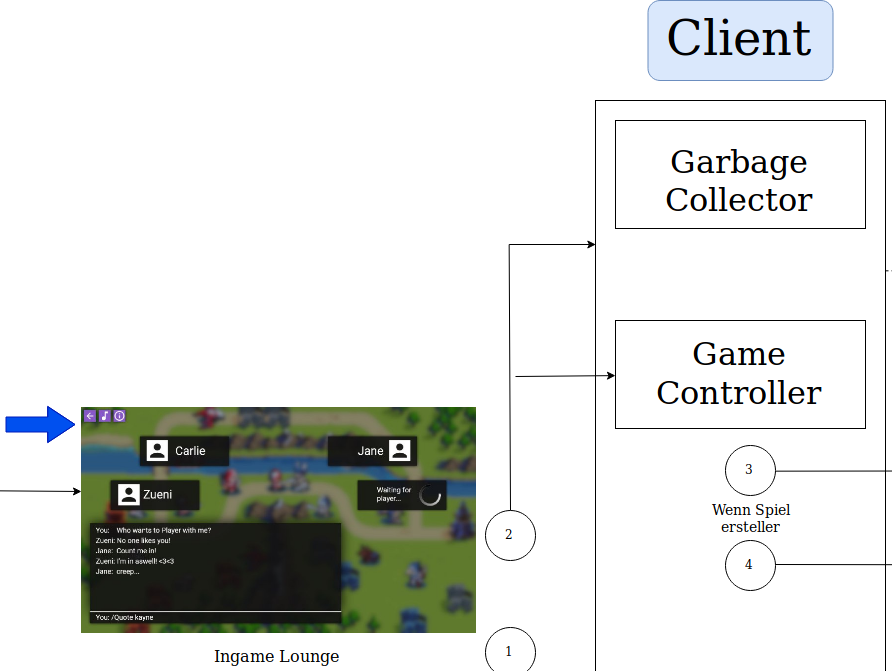
\includegraphics[width=0.7\textwidth]{BackToLobby2.png}
			\caption{Domain Story Benachrichtigung der Spielcontroller}
			\label{DomainStoryZurueckController}
		\end{figure} 
		\begin{figure}[H] 
			\centering
			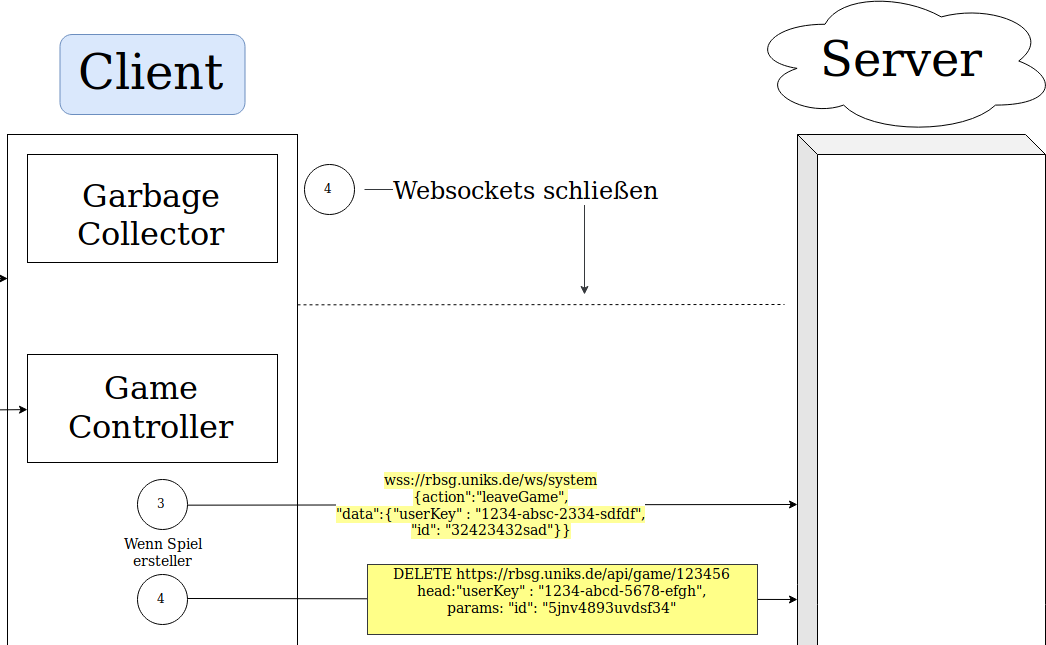
\includegraphics[width=0.7\textwidth]{BackToLobby3.png}
			\caption{Domain Story DELETE Anfrage an den Server}
			\label{DomainStoryZurueckDelete}
		\end{figure} 
		\subsubsection{Armeemanager - Erstellen und Speichern einer Armee}
		Eine weitere Anforderungen f�r das zweite Release ist, Armeen konfigurieren und speichern zu k�nnen, sowohl lokal als auch auf dem Server. In Abb. \ref{DomainStoryArmyManager1} wird der Szenenwechsel nach Bet�tigen des Armee erstellen-Buttons dargestellt (1). Im ArmyBuilder k�nnen anhand einer Einheitenauswahl Armeen konfiguriert werden. Anschlie�end wird durch Bet�tigen des Speichern-Buttons ein Army Manager Objekt angewiesen, den Speicher-Event auszuf�hren (2). Siehe dazu Abb. \ref{DomainStoryArmyManager2}. Der Army Manger sendet die aktuelle Armeekonfiguration im JSON-Format zum einen an den Server. Zum anderen wird die Armee lokal als JSON-Datei im daf�r vorgesehenen Verzeichnis gespeichert (3). Dieser Vorgang wird in Abb. \ref{DomainStoryArmyManager3} abgebildet.
			\begin{figure}[H] 
				\centering
				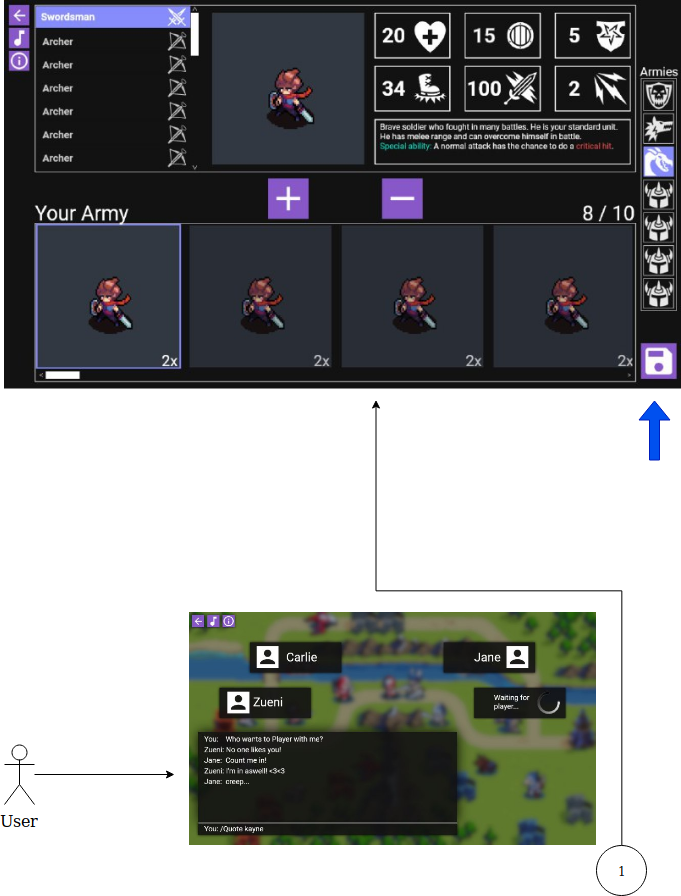
\includegraphics[width=0.5\textwidth]{ArmyManager1.png}
				\caption{Domain Story Wechsel in den ArmyBuilder}
				\label{DomainStoryArmyManager1}
			\end{figure}
			\begin{figure}[H] 
				\centering
				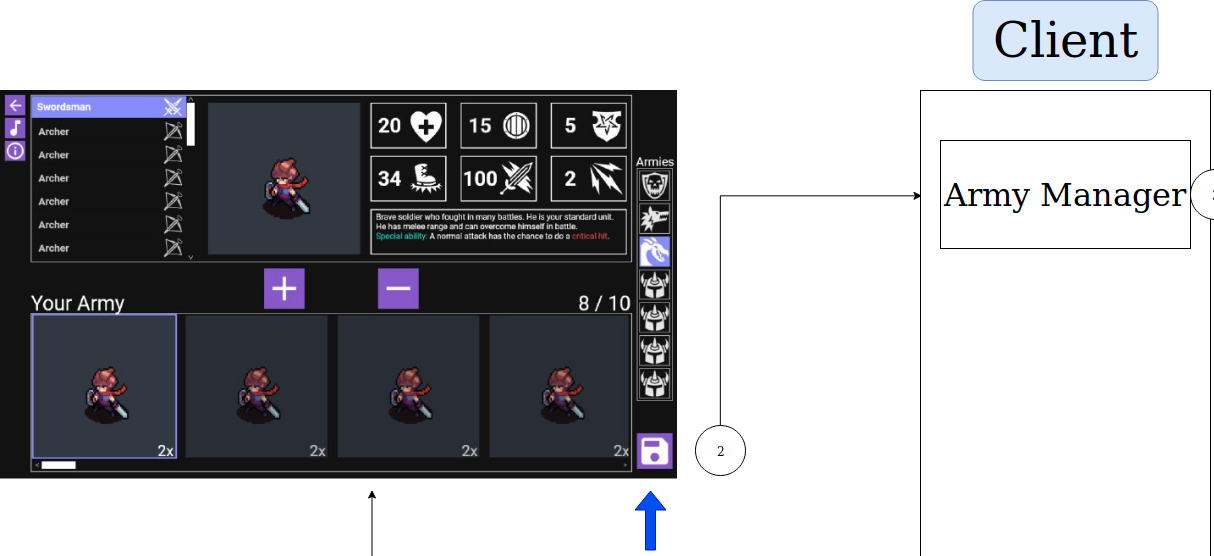
\includegraphics[width=0.7\textwidth]{ArmyManager2.png}
				\caption{Domain Story Speichern einer Armee}
				\label{DomainStoryArmyManager2}
			\end{figure}
			\begin{figure}[H] 
				\centering
				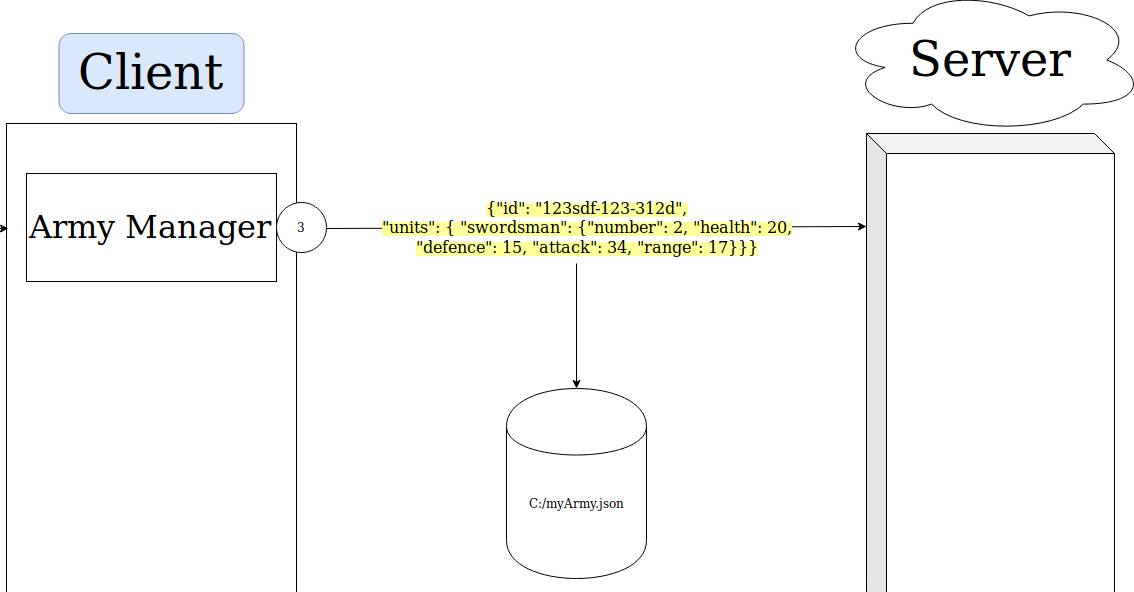
\includegraphics[width=0.7\textwidth]{ArmyManager3.png}
				\caption{Domain Story Speichern der Armee auf dem Server und lokal}
				\label{DomainStoryArmyManager3}
			\end{figure}
		\subsubsection{Client - Nachrichten des Server m�ssen korrekt verarbeiten} Nach einem Spielbeitritt sollen alle eingehenden Nachrichten vom Server korrekt verarbeitet werden. Dazu geh�ren der Spielbeitritt weiterer Spieler sowie das initiale Spielgeschehen. In Abb. \ref{DomainStoryHandler2} werden eingehende Servernachrichten (1)-(3) dargestellt. Diese werden von jeweils von einem eigenen Handler-Objekt verarbeitet. Die Handler setzen die Servernachrichten im Datenmodell und im GUI der Applikation um (1)-(2), wie gezeigt in Abb. \ref{DomainStoryHandler1}.
			\begin{figure}[H] 
				\centering
				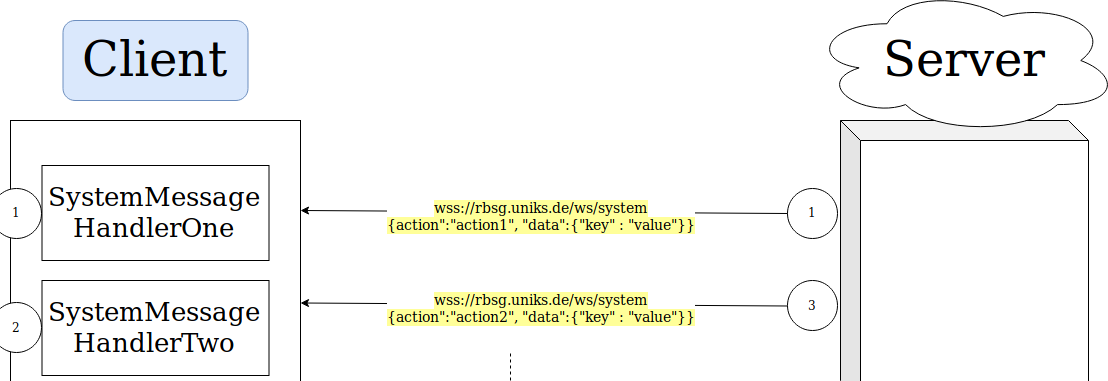
\includegraphics[width=0.7\textwidth]{Handler2.png}
				\caption{Domain Story Eingehend Servernachrichten}
				\label{DomainStoryHandler2}
			\end{figure}
			\begin{figure}[H] 
				\centering
				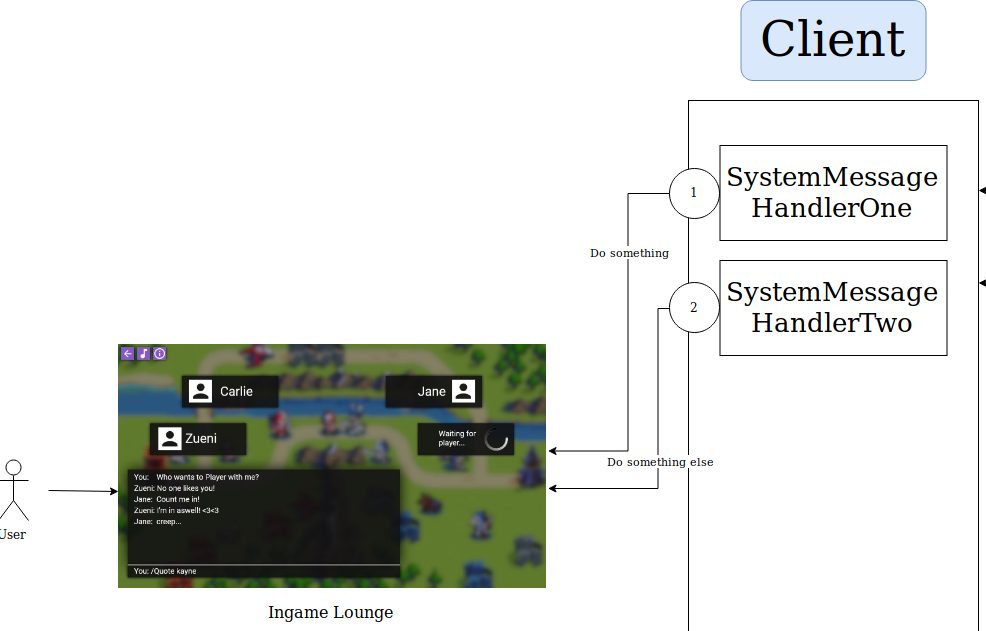
\includegraphics[width=0.7\textwidth]{Handler1.png}
				\caption{Domain Story System message handler}
				\label{DomainStoryHandler1}
			\end{figure}
		\subsubsection{Ingame Chat}
		Die Abb. \ref{DomainStoryChat1} zeigt eine eingehende Chatnachricht, die im allgemeinen Channel versendet wurde (1). Diese wird vom Chat-Websocket unseres Client empfangen und an den entsprechenden Chat-Controller weitergereicht (2). Anschlie�end wird die Chatnachricht vom Chat-Controller im Chatfenster angezeigt (3) (Abb. \ref{DomainStoryChat2}).
			\begin{figure}[H] 
				\centering
				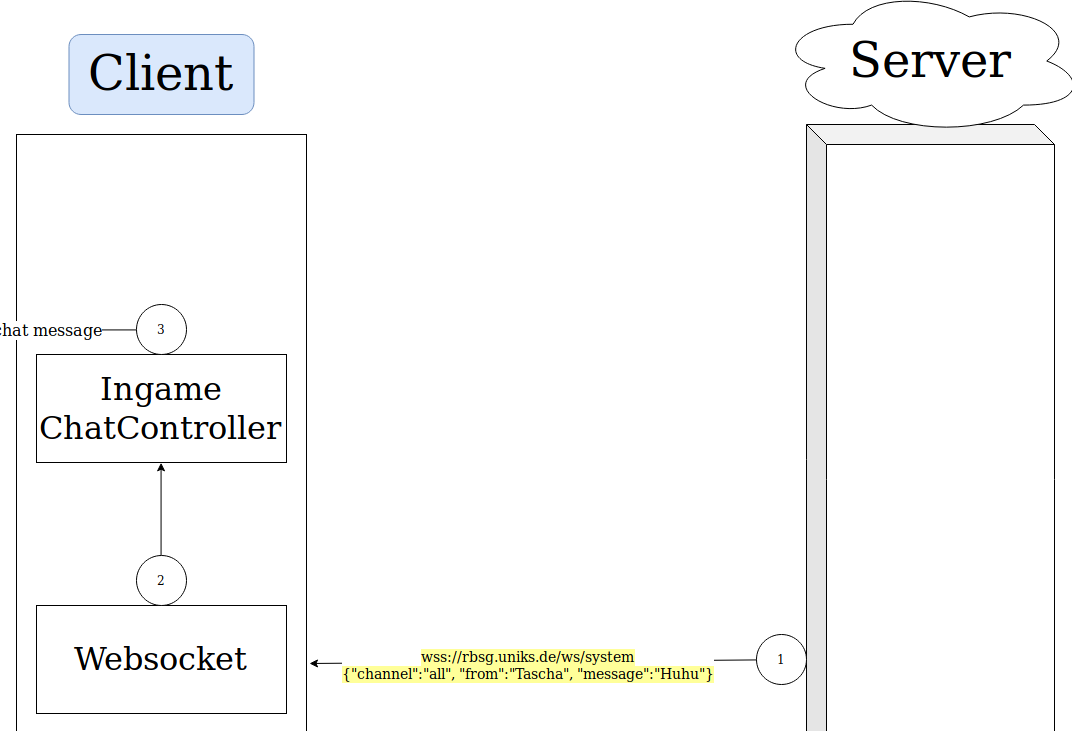
\includegraphics[width=0.7\textwidth]{Chat1.png}
				\caption{Domain Story Eingehende Chatnachricht}
				\label{DomainStoryChat1}
			\end{figure}
			\begin{figure}[H] 
				\centering
				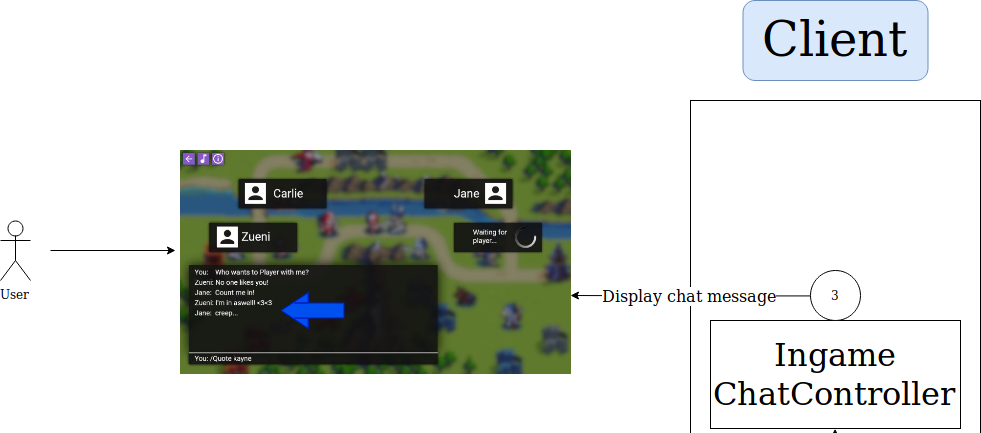
\includegraphics[width=0.7\textwidth]{Chat2.png}
				\caption{Domain Story Anzeigen der Chatnachricht}
				\label{DomainStoryChat2}
			\end{figure}
	\section{Sprint \RN{3}}
		Der dritte Sprint dauert vom 10.06.2019 bis zum 25.06.2019. Es wurden f�r den Sprint 130 Storypoints gesch�tzt.
		\subsection{Sprintziel}
		Das Sprintziel ist im Jira mit \glqq Die Ausgangsituation zum Spielen erreichen.\grqq definiert. Darunter f�llt:
		\begin{itemize}
			\item Erstellen von Armeen
			\item Speichern und Laden von Armeen
			\item Ausw�hlen einer Armee
			\item Verarbeiten der Initialen Servernachrichten
			\item Anzeigen des Waiting Rooms
		\end{itemize}
		\subsection{User Stories}
		\label{UserStoriesSprint3}
		Die Titel der User Stories ergeben sich nach folgendem Muster. Zuerst wird die Priorit�t f�r das Release genannt. Hierbei unterteilen wir in \glqq Core\grqq, f�r Hauptfeatures, und in \glqq Optional\grqq, f�r Zusatzfeatures. Danach folgt der zugeh�rige Bereich zum Beispiel \glqq Lobby\grqq. Zuletzt folgt eine kurze Beschreibung des Features. Dies wird im Folgendem beibehalten. Es wurde vom Team entschieden, dass im zweiten Release ein Story Point einem Arbeitsaufwand von einer Stunde entspricht.
		
		\subsubsection{Core - ArmyBuilder - Laden der Armeen}
		\paragraph{Ziel} Die Aufgabe besteht darin das Laden der gespeicherten Armeen lokal und serverseitig zu realisieren.
		\paragraph{Story} Albert befindet sich im Login Bereich. Albert loggt sich erfolgreich beim Spiel ein. Die lokal/auf dem Server gespeicherten Armeen werden geladen. Albert befindet sich in der Lobby, die geladenen Armeen werden in der Armeenliste angezeigt.
		\paragraph{Zugeteilter Entwickler} Als Entwickler wurde Tobias Klipp eingeteilt, da dieser auch das Speichern der Armeen �bernimmt.
		\paragraph{Sch�tzung}
		Das Feature wurde auf f�nf Story Points gesch�tzt.
		\paragraph{Verlauf der Entwicklung} Das Feature wurde im Verlauf der Entwicklung auf Omar Sood und Tobias Klipp aufgeteilt. Tobias �bernimmt dabei das Laden der Lokalen Speicherst�nde und Omar das Laden der St�nde vom Server. Dies wurde vollzogen, da Tobias sich erst in die Projektstruktur einarbeiten musste, da er im letzten Release Product Owner war. Das Feature wurde nicht im dritten Sprint abgeschlossen und wurde deshalb in den vierten Sprint �bernommen.
		
		\subsubsection{Core - ArmyBuilder - Speichern der Armeen}
		\paragraph{Ziel} Der Entwickler soll das Speichern von Armeen lokal und serverseitig implementieren.
		\paragraph{Story} Albert befindet sich in dem ArmyBuilder. Albert hat eine Armee eine konfiguriert. Albert klickt auf den Speichern Button. Die Armeen werden lokal und auf dem Server gespeichert.
		\paragraph{Zugeteilter Entwickler} Diese Story bearbeitet Tobias Klipp, um sich in mit der REST Kommunikation vertraut zu machen.
		\paragraph{Sch�tzung}
		Da das Feature von den Entwicklern als komplex eingesch�tzt wurde, erhielt es 13 Story Points.
		\paragraph{Verlauf der Entwicklung} Die Realisierung des Speicherns der Armeen nahm deutlich mehr Zeit in Anspruch als geplant, da Tobias sich erst in die REST-Kommunikation einarbeiten mussten und auch noch nicht mit der Quelltextbasis vertraut war. Dies fiel nach der Teambesprechung am 14.06.2019 auf. Daraufhin wurd Tobias vom Scrum Master sowie einem Entwickler eingewiesen. Dieses Feature wurde nicht im dritten Sprint beendet und wurd in den vierten Sprint �bernommen.
		
		\subsubsection{Core - ArmyBuilder - Auswahl einer Einheit}
		\paragraph{Ziel} Ziel der Story ist es die Einheitenauswahl in einer Liste darzustellen. Wird eine Einheit ausgew�hlt, soll eine Detailansicht dieser Einheit angezeigt werden.
		\paragraph{Story} Albert befindet sich im ArmyBuilder. Es wird die Einheitenliste mit Einheiten angezeigt. Albert klickt eine Einheit aus der Liste an. Die Einheit wird ausgew�hlt und es wird eine Detail View zur Einheit angezeigt.
		\paragraph{Zugeteilter Entwickler} Die Story wird von Omar Sood bearbeitet, da dieser f�r die Oberfl�che und Logik des ArmyBuilders zust�ndig ist.
		\paragraph{Sch�tzung}
		Das Feature wurde auf f�nf Story Points gesch�tzt.
		\paragraph{Verlauf der Entwicklung} Die ben�tigte Zeit f�r die Entwicklung waren am Ende ca. 10h, da sich der Entwickler erst in einige JavaFx\footnote{Graphische Oberfl�chenbibilthek f�r Java} Themen einarbeiten musste. Des Weiteren umfasste die Aufgabe auch das Erstellen der Liste und die Serverkommunikation. Die Zeit ist somit nachvollziehbar und wurde vom Team falsch eingesch�tzt.
		
		\subsubsection{Core - ArmyBuilder - Entfernen der Einheiten}
		\paragraph{Ziel} Ziel ist es eine Einheit aus einer Armee zu entfernen.
		\paragraph{Story} Albert befindet sich im ArmyBuilder. Es ist eine Einheit in \glqq Deiner Armee \grqq ausgew�hlt. Albert klickt auf den Entfernen-Button. Die Einheit wird aus \glqq Deiner Armee \grqq entfernt.
		\paragraph{Zugeteilter Entwickler} Die Story wird von Omar Sood bearbeitet, da dieser f�r die Oberfl�che und Logik des ArmyBuilders zust�ndig ist.
		\paragraph{Sch�tzung}
		Das Feature wurde auf f�nf Story Points gesch�tzt.
		\paragraph{Verlauf der Entwicklung} Omar ben�tigte nur 39min f�r das Feature. Da in einer anderen User Story die notwendige Programmlogik f�r dieses Feature vorbereitet wurde.
		
		\subsubsection{Core - ArmyBuilder - zur�ck in die Lobby navigieren}
		\paragraph{Ziel} Man soll den ArmyBuilder verlassen k�nnen und dann zur�ck in die Lobby kommen.
		\paragraph{Story} Albert befindet sich im ArmyBuilder. Es ist ein Zur�ck-Button im ArmyBuilder vorhanden. Albert klickt auf den Zur�ck-Button. Albert kommt zur�ck in die Lobby.
		\paragraph{Zugeteilter Entwickler} Da Keanu St�ckrad bereits vorher andere Szenenwechsel realisiert hat, fiel Ihm diese Task zu.
		\paragraph{Sch�tzung}
		Das Feature wurde auf 3 Story Points gesch�tzt.
		\paragraph{Verlauf der Entwicklung} 
		Die Entwicklung verlief schneller als erwartet und wurde nach 1h abgeschlossen.
		
		\subsubsection{Core - ArmyBuilder - L�schen der Armee (Clear)}
		\paragraph{Ziel} Im ArmyBuilder soll ein Button implementiert werden mit dem man eine Armee komplett leeren kann.
		\paragraph{Story}Albert befindet sich in dem ArmyBuilder. Es ist eine Armee mit Einheiten ausgew�hlt. Albert klickt auf den Trash-Button. Alle Einheiten der ausgew�hlten Armee werden aus dieser entfernt. Es wird noch keine �nderung gespeichert.
		\paragraph{Zugeteilter Entwickler} Diese Aufgabe hat Tobias Klipp bekommen, da er das Laden und Speichern der Armee realisiert.
		\paragraph{Sch�tzung}
		Das Feature wurde auf 1 Story Points gesch�tzt.
		\paragraph{Verlauf der Entwicklung} 
		Das Feature wurde nicht im dritten Sprint abgeschlossen und wurde deshalb in den vierten Sprint �bernommen.
		
		\subsubsection{Core - ArmyBuilder - Info �ber Attribute}
		\paragraph{Ziel} Im ArmyBuilder soll eine Anzeige mit Informationen zu den Attributen der Einheiten geben.
		\paragraph{Story}Albert befindet sich in dem ArmyBuilder. Der ArmyBilder enth�lte einen Info-Button. Albert klick auf den Info-Button. Es �ffnet sich ein Dialog mit entsprechenden Informationen zu den Attributen und der Erkl�rung zu weiteren Symbolen.
		\paragraph{Zugeteilter Entwickler} Die Task wurde von Keanu St�ckrad bearbeitet.
		\paragraph{Sch�tzung}
		Das Feature wurde auf 3 Story Points gesch�tzt.
		\paragraph{Verlauf der Entwicklung} 
		Die Entwicklung hat 2 Stunden l�nger in Anspruch genommen, da der Entwickler mehr Zeit f�r das Aussehen der Oberfl�che ben�tigte.
		
		\subsubsection{Optional - ArmyBuilder - Musik an/aus}
		\paragraph{Ziel} Im ArmyBuilder soll es einen Button geben um die Musik an- und auszuschalten. 
		\paragraph{Story} Zwei Stories zusammengefasst da sich beide Stories von den Arbeitsbereichen zu stark �berschneiden. \\ \ \\ Albert befindet sich in dem ArmyBuilder. Die Musik l�uft. Albert nervt die Musik. Albert klickt auf den Musik-Button. Die Musik geht aus. \\ Albert hat wieder Lust auf Musik. Albert klickt auf den Musik-Button. Die Musik geht wieder an.
		\paragraph{Zugeteilter Entwickler} Die Task wurde von Keanu St�ckrad bearbeitet, da dieser schon das Abspielen der Musik implementiert hat.
		\paragraph{Sch�tzung}
		Das Feature wurde auf 1 Story Points gesch�tzt.
		\paragraph{Verlauf der Entwicklung} 
		Die Entwicklung verlief mit 30 Minuten f�r das Feature schneller als geplant.
		
		\subsubsection{Optional - Waiting Room - Anzeigen der Karte (Preview)}
		\paragraph{Ziel} Im Warteraum soll es eine Vorschau f�r die Karte des kommenden Spiels geben.
		\paragraph{Story} Albert befindet sich in der Lobby. Albert tritt einem Spiel aus der Spieleliste bei. Albert wird beim Spiel angemeldet und befindet sich nun im Waiting Room. Es wird eine Vorschau f�r das kommende Spielfeld angezeigt.
		\paragraph{Zugeteilter Entwickler} Diese Story wurde von Jan M�ller bearbeitet.
		\paragraph{Sch�tzung}
		Das Feature wurde auf 3 Story Points gesch�tzt, da es auf das Anzeigen des Spielfeldes aufbaut und sich daran orientiert werden kann.
		\paragraph{Verlauf der Entwicklung} 
		Diese Story wurde im dritten Sprint begonnen, konnte jedoch nicht abgeschlossen werden, da hier auf die Fertigstellung der Spielkarte gewartet werden musste. Die Story wurde in den vierten Sprint mitgenommen.
		
		\subsubsection{Core - Waiting Room - Anzeigen des Waiting Rooms (neues Layout)}
		\paragraph{Ziel} Durch das zweite Release gab es neue Anforderungen an den Warteraum, weshalb das Layout des Warteraums angepasst werden musste.
		\paragraph{Story} Albert befindet sich in der Lobby. Albert tritt einem Spiel aus der Spieleliste bei. Es wird der Waiting Room f�r das Spiel angezeigt nach dem neuen Layout (Mockup).
		\paragraph{Zugeteilter Entwickler} Diese Aufgabe wurde Keanu St�ckrad zugeteilt, da er im letzten Release bereits begonnen hat den Waiting Room zu implementieren.
		\paragraph{Sch�tzung}
		Das Feature wurde auf f�nf Story Points gesch�tzt.
		\paragraph{Verlauf der Entwicklung} 
		Die Anpassungen erwiesen sich als zeitaufw�ndiger, da der Entwickler Probleme mit der Anordnung der einzelnen Elemente hatte. Es wurden insgesamt 9 Stunden daf�r ben�tigt.
		
		\subsubsection{Core - Lobby - Auswahl der Armee }
		\paragraph{Ziel} Es soll m�glich sein in der Lobby eine Armee auszuw�hlen. 
		\paragraph{Story} Albert befindet sich in der Lobby. Es wird die Armeeauswahl angezeigt. Albert klickt eine Armee an. Die Armee wird f�r das kommende Spiel ausgew�hlt.
		\paragraph{Zugeteilter Entwickler} Omar Sood wurde dieser Aufgabe zugeteilt, da von Ihm der Armeeauswahl im ArmyBuilder bereits implementiert wurde.
		\paragraph{Sch�tzung}
		Das Feature wurde auf 1 Story Points gesch�tzt.
		\paragraph{Verlauf der Entwicklung} 
		Die Aufgabe wurde innerhalb von 18 Minuten abgeschlossen, da viele Grundlagend bereits vorhanden waren.
		
		\subsubsection{Core - Ingame - Anzeigen der Spielfeldes}
		\paragraph{Ziel} Es soll das Spielfeld angezeigt werden.
		\paragraph{Story}Albert befindet sich im Waiting Room und es sind alle Spieler f�r ein Spiel anwesend. Das Spiel wird gestartet. Es wird das Spielfeld angezeigt.
		\paragraph{Zugeteilter Entwickler} Keanu St�ckrad bearbeitete diese Aufgabe.
		\paragraph{Sch�tzung}
		Das Feature wurde auf 3 Story Points gesch�tzt.
		\paragraph{Verlauf der Entwicklung} 
		F�r die Aufgabe wurden am Ende 7,5h ben�tigt, da es zum Zeitpunkt der Sch�tzung unklar war, welche Informationen �ber das Spielfeld vom Server gesendet werden. Die Sch�tzung der Aufgabe wurde vor Ver�ffentlichung der Serverdokumentation des zweiten Releases durchgef�hrt. Die Nachrichten des Servers werden in der Serverdokumentation nicht erl�utert, was das Sch�tzen der Task erschwert.
		
		\subsubsection{Optional - Ingame - Zoomen auf dem Spielfeld}
		\paragraph{Ziel} Es soll ein Vergr��ern und Verkleinern der Spielkarte m�glich sein.
		\paragraph{Story}Albert befindet sich in einem Spiel welches bereits gestartet ist. Es ist ein Vergr��ern-Button vorhanden. Albert klickt auf den Verkleinern-Button. Das Spielfeld wird um eine Stufe herangezoomt.
		\paragraph{Zugeteilter Entwickler} Diese Aufgabe bearbeite Keanu St�ckrad, da er auch f�r die Implementierung des Spielfeldes verantwortlich war.
		\paragraph{Sch�tzung}
		Das Feature wurde auf 15 Story Points gesch�tzt, da es noch unklar war wie man das Zoomen realisiert werden kann.
		\paragraph{Verlauf der Entwicklung} 
		Das Feature wurde bereits in diesem Sprint begonnen, konnte jedoch nicht fertig gestellt werden. Es wird in den vierten Sprint �bernommen.
		
		\subsubsection{Core - Ingame - Spiel verlassen}
		\paragraph{Ziel} Es soll m�glich sein ein Spiel zu verlassen.
		\paragraph{Story} Albert befindet sich in einem gestartetem Spiel. Albert hat den Early Rush vermasselt. In der Ingame Scene ist ein Leave-Game-Button vorhanden. Albert klickt auf den Leave-Game-Button und verl�sst das Spiel ordnungsgem��. Albert kommt zur�ck in die Lobby.
		\paragraph{Zugeteilter Entwickler} Als Entwickler wurde Keanu St�ckrad dieser Aufgabe zugeteilt.
		\paragraph{Sch�tzung}
		Das Feature wurde auf 3 Story Points gesch�tzt
		\paragraph{Verlauf der Entwicklung} 
		Das Feature wurde bereits in diesem Sprint begonnen, konnte jedoch noch nicht abgeschlossen werden. Es wurde in den vierten Sprint verschoben.
		
		\subsubsection{Core - ArmyBuilder - Hinzuf�gen der Einheiten}
		\paragraph{Ziel} Es soll die ausgew�hlte Einheit der Armeeliste hinzugef�gt werden.
		\paragraph{Story} Albert befindet sich im ArmyBuilder. Er hat eine Einheit ausgew�hlt. Albert klickt auf den Hinzuf�gen-Button Die ausgew�hlte Einheit wird der ausgew�hlten Armee hinzugef�gt.
		\paragraph{Zugeteilter Entwickler} Die Story wird von Omar Sood bearbeitet, da dieser f�r die Oberfl�che und Logik des ArmyBuilders zust�ndig ist.
		\paragraph{Sch�tzung}
		Das Feature wurde auf 13 Story Points gesch�tzt
		\paragraph{Verlauf der Entwicklung} 
		Die Entwicklung verlief schneller als geplant, da bereits Techniken aus vorhergehende Tasks angewandt werden konnten. Es wurde Insgesamt nur 7 Stunden und 23 Minuten ben�tigt.
		
		\subsubsection{Core - Waiting Room - Spiel beitreten}
		\paragraph{Ziel} Es soll erfolgreich einem Spiel beigetreten werden und der Waiting Room angezeigt werden.
		\paragraph{Story} Albert befindet sich in der Lobby. Albert hat eine Armee ausgew�hlt und klickt auf Spiel beitreten. Albert befindet sich nun im Waiting Room. Die Verbindung wird korrekt aufgebaut und es k�nnen Nachrichten empfangen werden.
		\paragraph{Zugeteilter Entwickler} Jan M�ller wurde diese Aufgabe zugeteilt.
		\paragraph{Sch�tzung}
		Das Feature wurde auf 16 Story Points gesch�tzt, da die Verarbeitung der Servernachrichten als komplex angesehen wurden. Eine Sch�tzung war f�r diese Aufgabe schwer, da die Serverdokumentation keine Aussage �ber die eingehenden Nachrichten macht.
		\paragraph{Verlauf der Entwicklung} 
		Die Implementierung verlief ohne Komplikationen. Die Task ben�tigte insgesamt 15,5h zur Bearbeitung, womit wir leicht unter der Sch�tzung lagen. Die Story wurde also vom Team gut eingesch�tzt.
		
		\subsubsection{Core - Waiting Room - Chat}
		\paragraph{Ziel} Im Waiting Room soll ein Chat vorhanden sein
		\paragraph{Story} Albert befindet sich im Waiting Room eines Spiels. Albert schreibt ein Nachricht in den Game-Chat. Die Nachricht wird im Game-Chat angezeigt und die Nachricht wird an die anderen Spieler versendet.
		\paragraph{Zugeteilter Entwickler} Jan M�ller wurde diese Aufgabe zugeteilt, da Jan im letzten Release schon f�r den Chat in der Lobby zust�ndig war.
		\paragraph{Sch�tzung}
		Das Feature wurde von Jan auf 13 Story Points gesch�tzt, da er die meiste Erfahrung mit dem Chat hat.
		\paragraph{Verlauf der Entwicklung} 
		Die Story wurde zeitaufw�ndiger eingesch�tzt, als diese am Ende war. Es wurde 13h prognostiziert, von den wir am Ende nur 6,5h ben�tigten. Das Team hat die Aufgabe �bersch�tzt, da die Teammitglieder nicht sicher waren, wie die Interaktion mit dem Game-Websocket ausfallen wird.
		
		\subsubsection{Appearance - ArmyBuilder}
		\paragraph{Ziel} Es soll der AmryBuilder an das Dark Theme angepasst werden.
		\paragraph{Story} Albert befindet sich in der Lobby. Albert klickt auf den ArmyBuilder Button. Albert befindet sich nun im ArmyBuilder und es sind alle n�tigen Daten geladen und werden angezeigt. Der ArmyBuilder wird entsprechend dem Style der Mockups angezeigt.
		\paragraph{Zugeteilter Entwickler} Als Entwickler wurde Keanu St�ckrad diese Aufgabe zugewiesen.
		\paragraph{Sch�tzung}
		Das Feature wurde auf 8 Story Point gesch�tzt.
		\paragraph{Verlauf der Entwicklung} 
		Diese Story wurde in den vierten Sprint verschoben, da wir uns im dritten Sprint st�rker auf die Funktionalit�t fokussiert haben. 
		
		\subsubsection{Core - ArmyBuilder - In den ArmyBuilder navigieren}
		\paragraph{Ziel} In der Lobby soll ein Button vorhanden sein, mit welchem man in den ArmyBuilder navigieren kann.
		\paragraph{Story} Albert befindet sich in der Lobby. In der Lobby ist ein ArmyBuilder-Button vorhanden. Albert klickt auf den ArmyBuilder-Button. Albert kommt in den Army Builder.
		\paragraph{Zugeteilter Entwickler} Die Story wird von Omar Sood bearbeitet, da dieser f�r die Oberfl�che und Logik des ArmyBuilders zust�ndig ist.
		\paragraph{Sch�tzung}
		Das Feature wurde auf 3 Story Points gesch�tzt.
		\paragraph{Verlauf der Entwicklung} 
		Die Entwicklung des Features dauerte 4 Stunden und 7 Minuten. Die Entwickler haben, die Aufgaben leicht untersch�tzt.
		
		\subsubsection{Core - ArmyBuilder - Ausw�hlen einer Armee}
		\paragraph{Ziel} Im ArmyBuilder soll eine Auswahl f�r die Armeen vorhanden sein.
		\paragraph{Story} Albert befindet sich in der ArmyBuilder. Es ist eine Liste der Armeen vorhanden. Albert klickt auf eine Armee (w�hlt diese aus). Die Armee wird selektiert und entsprechend in der Armee�bersicht angezeigt.
		\paragraph{Zugeteilter Entwickler} Die Story wird von Omar Sood bearbeitet, da dieser f�r die Oberfl�che und Logik des ArmyBuilders zust�ndig ist.
		\paragraph{Sch�tzung}
		Die Story wurde auf f�nf Story Points gesch�tzt.
		\paragraph{Verlauf der Entwicklung} 
		Die Entwicklung dauerte 1 Stunde und 58 Minuten. Der Entwickler war schneller fertig als erwartet. Dies lag daran, dass andere Tasks bereits Grundlagen f�r die Task gaben und somit die Implementierung schneller m�glich war.
		\subsection{Tasks}
		Neben User Stories, die weiter in Unteraufgaben aufgeteilt sind, wurden einzelne Tasks vom Scrum Master erstellt, die keiner User Story zugeordnet wurden. Diese Tasks konnten nicht direkt in eine Aktion des Nutzers �bersetzt werden und waren rein technischer Natur, ohne Bezug zur graphischen Benutzeroberfl�che. Auf einzelne Tasks ist es in Jira nicht m�glich, Story Points zu sch�tzen. Im Verlauf des zweiten Releases wurden Zeitsch�tzungen erg�nzt.
		\subsubsection{Task - Tests optimieren}
		\paragraph{Ziel} Die Tests der graphischen Oberfl�che der Applikation sollten in Bezug auf ihre Ausf�hrungsdauer optimiert werden.
		\paragraph{Zugeteilter Entwickler} Der Task wird von Omar Sood bearbeitet.
		\paragraph{Verlauf der Entwicklung} 
		Die Implementierung dieses Task dauerte 25 Minuten. Es konnten keine Story Points auf diesen Task im Jira gesch�tzt. Intern wurde eine Arbeitsstunde f�r diesen Task veranschlagt. Damit ben�tigte der Entwickler weniger als die veranschlagte Zeit f�r diesen Taks.
		\subsubsection{Task - PR - stylingLoginCreate}
		\paragraph{Ziel} Aus dem ersten Release ist ein offener Pull Request �brig geblieben, der aufgrund von Konflikten nicht gemerged werden konnte. Der Task bestand darin, diese Konflikte zu beseitigen.
		\paragraph{Zugeteilter Entwickler} Keanu St�ckrad bearbeitete diesen Task.
		\paragraph{Verlauf der Entwicklung} 
		Mit 30 Minuten wurde dieser Taks schneller abgeschlossen, als die eine Stunde, die intern daf�r veranschlagt wurde.
		\subsubsection{Task - REST Kommunikation}
		\paragraph{Ziel} Die REST Kommunikation mit dem Server wird in unterschiedlichen Klassen mit Hilfe verschiedener Methoden gehandhabt. In diesem Task sollte die REST Kommunikation unserer Applikation vereinheitlicht werden.
		\paragraph{Zugeteilter Entwickler} Dieser Task wurde Omar Sood zugewiesen.
		\paragraph{Sch�tzung}
		Die Story wurde auf f�nf Zeitstunden gesch�tzt.
		\paragraph{Verlauf der Entwicklung} 
		Der Task wurde sehr niedrig priorisiert und wurde vom Entwickler im dritten Sprint nicht bearbeitet.
		\newpage
		
		\subsection{Zeit�bersicht}
		\begin{center}
				\begin{longtable}{p{6cm} c c c c }
					
					User Story	& Story Points & Soll Zeit & Ist Zeit & Entwickler\\
					\toprule
					\endhead
					Core - ArmyBuilder - Laden der Armeen & 5 & 5h & 16h 16min & Tobias Klipp \\ \hline 
					
					Core - ArmyBuilder - Speichern der Armeen & 13 & 13h & 34h 45min & Tobias Klipp\\ \hline
					
					Core - ArmyBuilder - Hinzuf�gen der Einheiten & 13 & 13h & 7h 23m & Omar Sood\\ \hline
					
					Core - ArmyBuilder - Entfernen der Einheiten & 5 & 5h & 39m & Omar Sood\\ \hline
					
					Core - ArmyBuilder - zur�ck in die Lobby navigieren & 3 & 3h & 1h & Keanu St�ckrad\\ \hline
						
					Core - ArmyBuilder - Info �ber Attribute & 3 & 3h & 5h & Keanu St�ckrad\\ \hline
			
					Core - Waiting Room - Anzeigen des Waiting Rooms (neues Layout) & 5 & 5h & 9h & Keanu St�ckrad\\ \hline
					
					Optional - ArmyBuilder - Musik an/aus & 1 & 1h & 30m & Keanu St�ckrad\\ \hline
					
					Core - Lobby - Auswahl der Armee  & 1 & 1h & 18m & Omar Sood\\ \hline
					
					Core - Ingame - Anzeigen der Spielfeldes & 3 & 3h & 7h 30m &  Keanu St�ckrad\\ \hline
					
					Core - ArmyBuilder - Auswahl einer Einheit & 5 & 5h & 9h 59m & Omar Sood\\ \hline
					
					Core - Waiting Room - Spiel beitreten & 16 & 16h & 15h 23m & Jan M�ller\\ \hline
					
					Appearance - ArmyBuilder & 8 & 8h & - & Tobias Klipp \\ \hline
					
					Core - Waiting Room - Chat & 13 & 13h & 6h 35m & Jan M�ller\\ \hline
					
					Core - ArmyBuilder - In den ArmyBuilder navigieren & 3 & 3h & 4h 7m & Omar Sood\\ \hline
					
					Core - ArmyBuilder- Ausw�hlen einer Armee & 5 & 5h & 1h 58m & Omar Sood \\
					\caption{�bersicht der Zeiten f�r den 3. Sprint} \\
				\end{longtable}
		\end{center}
			
		\subsection{Analyse des 3. Sprint}
		Der dritte Sprint wurde am 24.06.2019 beendet. Es wurden insgesamt 89 von 130 Story Points abgeschlossen. Die Planung konnte dabei nicht eingehalten werden. Die aufgetretenen Probleme werden im den folgenden Abschnitten erl�utert.
		
		\subsubsection{Burndown-Diagramm}
		Betrachtet man zun�chst das Burndown-Diagramm f�r den dritten Sprint, so nimmt in der ersten Woche die Anzahl der abgeschlossenen Story Points kaum zu. Ab der Mitte der zweiten Woche des Sprints beginnt der Graph schnell zu fallen und es endet mit den �brig gebliebenen 21 Story Points. Ein Grund f�r diesen Verlauf ist die FehleinSch�tzung des Teams der zu erledigenden Arbeit, so wurde zum Beispiel das Erstellen der Karte auf drei Story Points gesch�tzt. Am Ende wurde f�r diese Task insgesamt 7,5 Stunden ben�tigt. Dieses Problem trat diesen Sprint h�ufiger auf, da die Tasks vor Ver�ffentlichung der Serverdokumentation des zweiten Releases gesch�tzt wurden. Ein weiteres Problem, welches am Anfang des Sprints auftrat, waren die unklaren Anforderung an den Sprint, so wurden Features geplant welche mit dem damaligen Serverstand nicht m�glich waren. Darauf konnten wir jedoch gut reagieren, indem wir den Entwicklern erst Tasks zuwiesen, welche Sie bereits gut abarbeiten konnten. w�hrend dessen arbeiten wir die restlichen Tasks auf und passten Sie an den Serverstand an. Insgesamt k�nnen wir hier jedoch von einem guten Abarbeitung der Tasks sprechen, da die geforderten 80 Story Points erf�llt wurden, und einige Tasks sich im Nachhinein als noch aufw�ndiger heraus stellten. 
		
		\begin{figure}[H] 
			\centering
			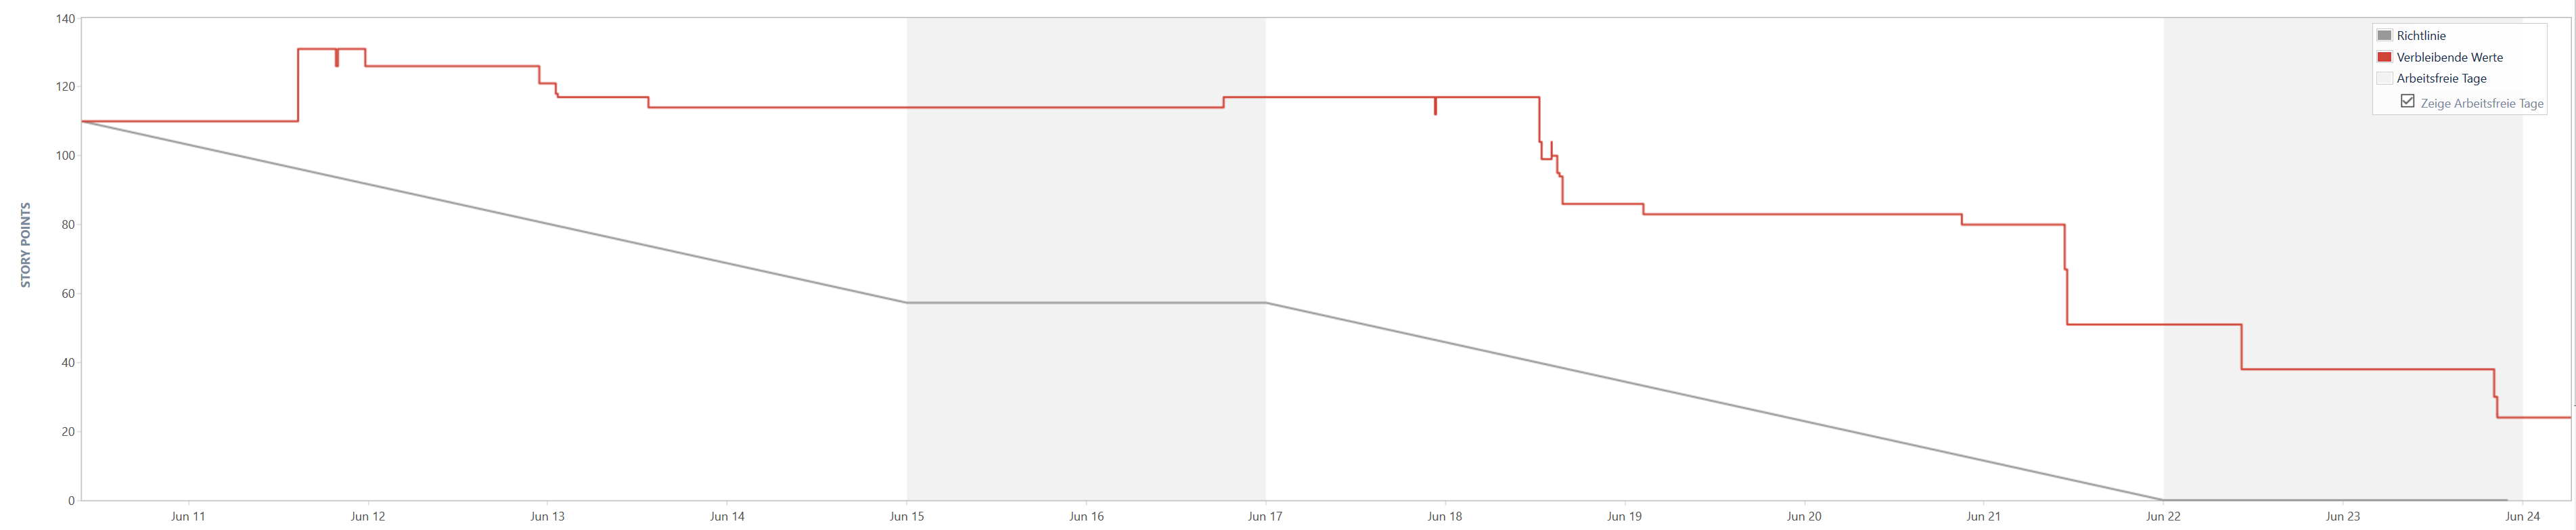
\includegraphics[width=0.8\textwidth]{BurndownChart_Sprint3.PNG}
			\caption{Burndown-Diagramm des Sprint 3}
			\label{BurndownSprint3}
		\end{figure}
		
		\subsubsection{Abgeschlossene Vorg�nge}
		
		In \Abb{AbgeschlosseneVorgaengeSprint3} sind die Abgeschlossenen Vorg�nge f�r den 3. Sprint zu sehen. Insgesamt wurden bereits ein Gro�teil der geforderten Features f�r de zweiten Release abgearbeitet. So sind bereits folgende Features vorhanden:
		
		\paragraph{Initiales Spielgeschehen anzeigen} Bei betreten des Waiting Rooms werden alle Nachrichten f�r das initiale Spielgeschehen verarbeitet. So erstellen wir basierend auf den erhaltenden Nachrichten ein Datenmodel. Aus diesem wird die Spielkarte mit Graphiken f�r die entsprechenden Felder generiert.
		
		\paragraph{Ingame Chat}
		Im Waiting Room ist bereits ein Chat vorhanden, in welchem man �ber einen General-Chat mit allen Spielern im Spiel chatten kann und auch in einem Privat-Chat mit anderen kommunizieren kann.
		
		\paragraph{Vom Waiting Room zur�ck in die Lobby}
		Dieses Feature wurde auch bereits Implementiert, ein Verlassen des Spiel ist �ber einen entsprechenden Button bereits m�glich.
		
		\paragraph{Erstellen und konfigurieren der eigenen Armeen}
		Eine Konfiguration der Armeen ist bereits vollst�ndig m�glich. Dabei ist wird das Limit von 10 Einheiten pro Armee eingehalten. Ein Speichern der Armeen ist bereits lokal und auf dem Server m�glich.
		
		\paragraph{Ein C0 Abdeckung von 60\%}
		Zum Ende des dritten Sprints ist eine Code Coverage von 69\% vorhanden. Siehe \Abb{CodeCoverageSprint3}.
		\begin{figure}[H] 
			\centering
			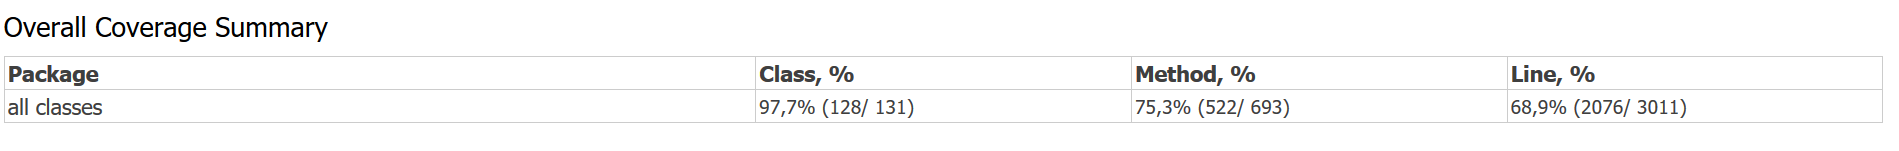
\includegraphics[width=1\textwidth]{Coverage_Sprint_3.PNG}
			\caption{Code Coverage vom 3. Sprint}
			\label{CodeCoverageSprint3}
		\end{figure}
		
		\begin{figure}[H] 
			\centering
			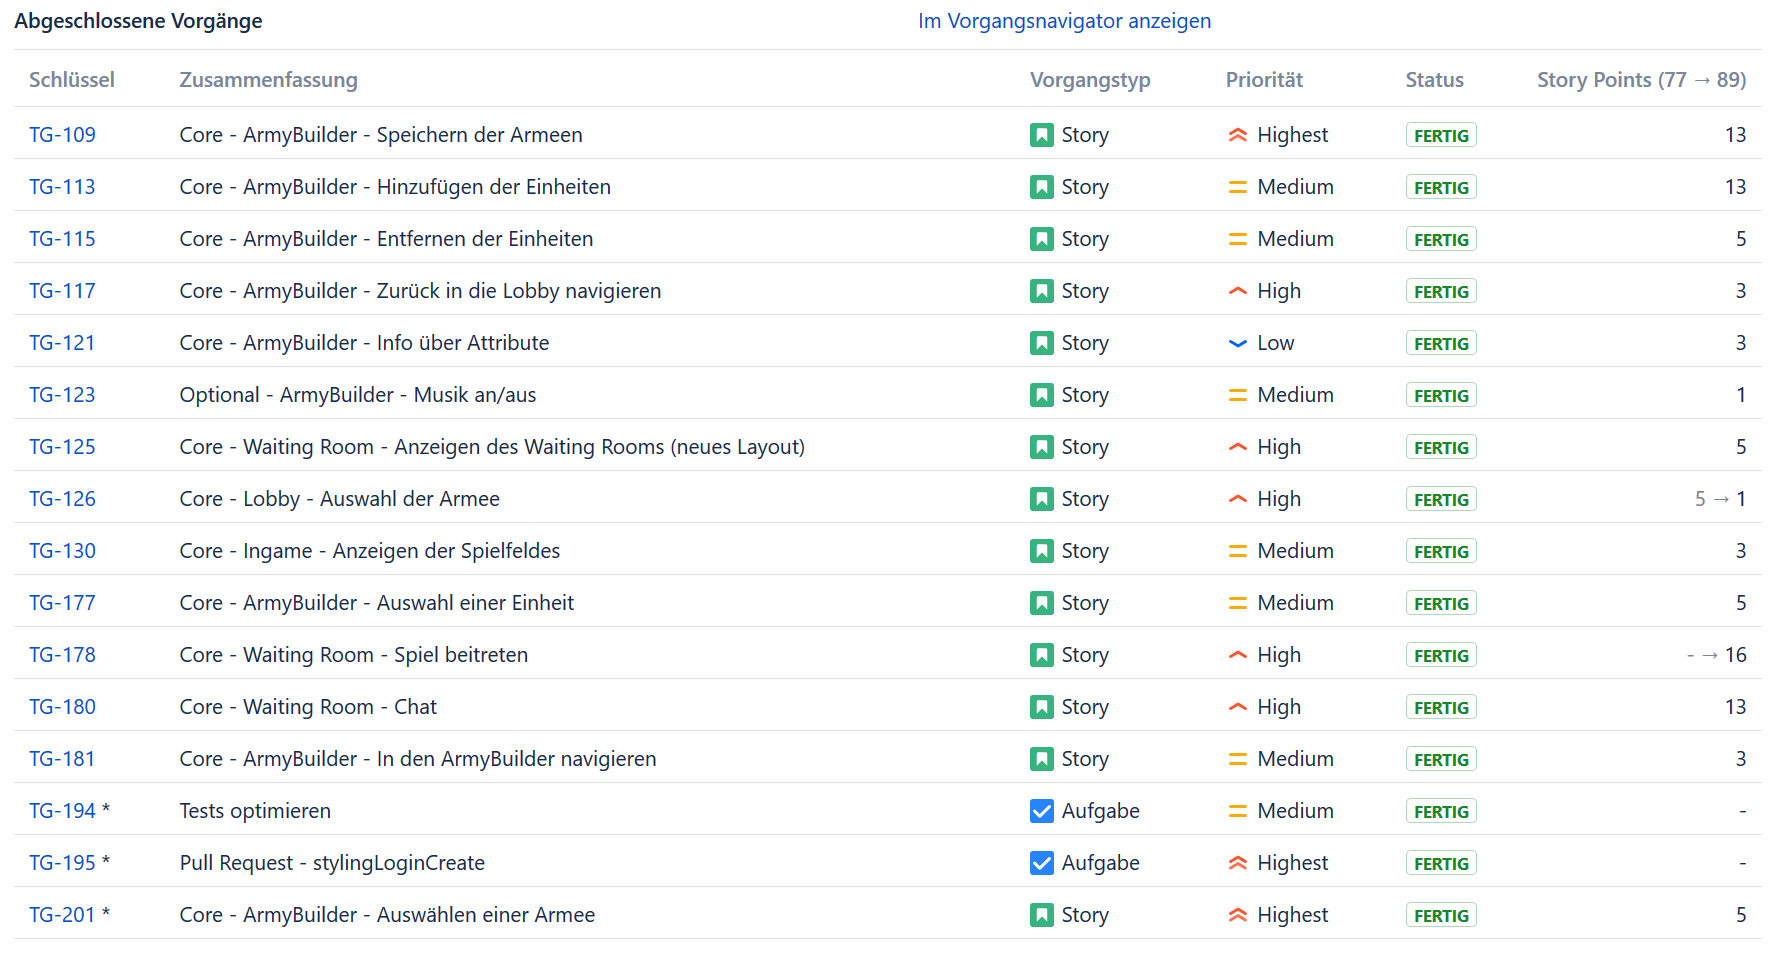
\includegraphics[width=1\textwidth]{Abschlossene_Vorgaenge_Sprint_3.png}
			\caption{Abgeschlossene Vorg�nge vom 3. Sprint}
			\label{AbgeschlosseneVorgaengeSprint3}
		\end{figure}
	
		\subsubsection{Nicht abgeschlossene Vorg�nge}
		Im dritten Sprint wurden Insgesamt 18 Story Points nicht abgeschlossen. Die entsprechenden Stories sind in \Abb{NichtAbgeschlosseneVorgaengeSprint3} aufgelistet. Die Tasks werden in den vierten Sprint verschoben. Bei den nicht abgeschlossenen Tasks fast ausschlie�lich um optionale oder weniger umfangreiche Aufgaben.
			
			\paragraph{Optional - Waiting Room - Anzeigen einer Karten Preview}
			Dieser Task konnte nicht abgeschlossen werden, da er durch die Fertigstellung der Spielkarte blockiert wurde. Dies verz�gerte aber nicht den Entwicklungsverlauf, da der Entwickler an anderen Aufgaben arbeiten konnte. 
			
			\paragraph{Optional - Ingame - Zoomen auf dem Spielfeld}
			Die Task wurde im dritten Sprint begonnen, aber nicht fertig gestellt. Dies kam durch den unerwarteten gr��eren Aufwand beim Erstellen des Spielfeldes.
			
			\paragraph{Core - Ingame - Spiel verlassen}
			Auch diese Task konnte auf Grund des h�heren Aufwands beim Erstellen des Spielfeldes noch nicht abgeschlossen werden. 
			
				\begin{figure}[H] 
					\centering
					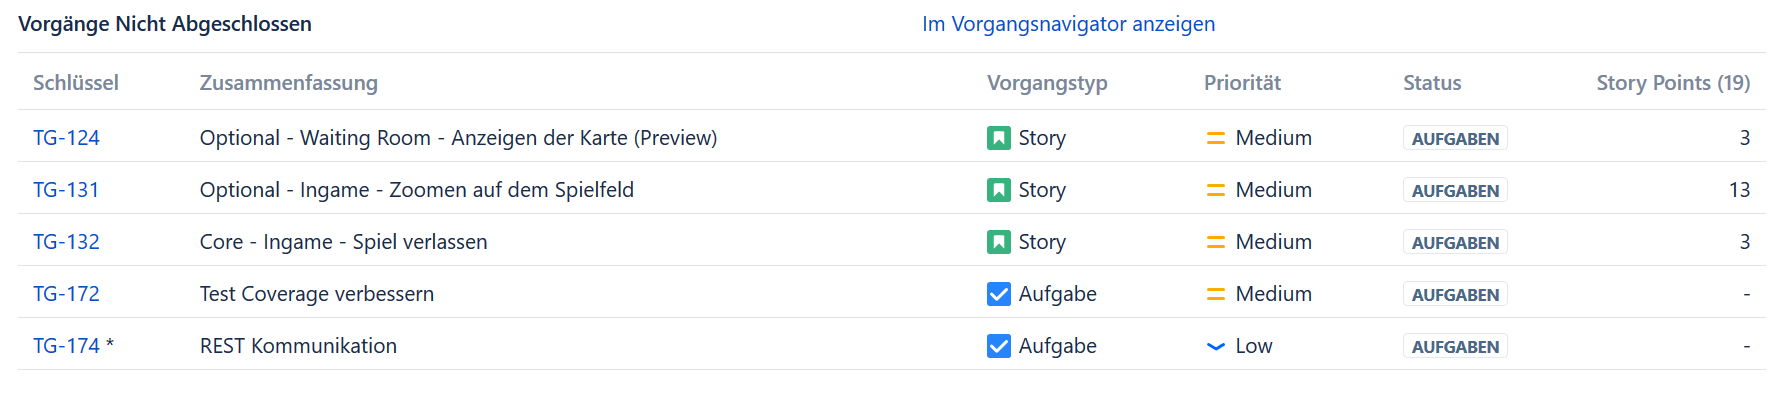
\includegraphics[width=0.8\textwidth]{Nicht_Abgeschlossene_Vorgaenge_Sprint_3.PNG}
					\caption{Nicht Abgeschlossene Vorg�nge vom 3. Sprint}
					\label{NichtAbgeschlosseneVorgaengeSprint3}
				\end{figure}
		\subsubsection{Entfernte Vorg�nge}
		Aus dem dritten Sprint wurden insgesamt 22 Story Points entfernt und in den vierten Sprint verschoben, da wir bereits schon absch�tzen konnten, dass diese nicht erreicht werden. 
			
			\paragraph{Core - ArmyBuilder - Laden der Armeen} \label{ProblemOne}Bei dieser Task wurde nach der ersten Woche deutlich, dass dies nicht mehr im dritten Sprint erreicht werden kann. Der Entwickler hat anfangs Schwierigkeiten, sich in das Projekt einzuarbeiten. Die Ursache daf�r war, dass der Entwickler im vorgehenden Release Product Owner war und so nicht mit der Quellcodebasis vertraut war. Dies wurde beim ersten Teammeeting erkannt. Als Reaktion darauf setzte sich der Entwickler und der Scrum Master zusammen, um den Quellcode aufzuarbeiten und so das entstandene Problem zu vermindern.
			
			\paragraph{Core - ArmyBuilder - L�schen der Armeen} Siehe \ref{ProblemOne} Core - ArmyBuilder - Laden der Armeen.
			
			\paragraph{Optional - Waiting Room - Anzeigen der ausgew�hlten Einheiten} Diese Task wurde erst im Verlauf des dritten Sprints erstellt. Da alle Entwickler ausgelastet waren und andere Tasks h�here Priorit�ten hatten wurde dieser verschoben.
			
			\paragraph{Appearance - Army Builder} Im dritten Sprint war es uns wichtig Funktionalit�ten bereit zu stellen. Deswegen wurden andere Tasks zuerst abgearbeitet. Das Anpassen der Oberfl�che wurde auf den n�chsten Sprint verlegt.
			\begin{figure}[H] 
				\centering
				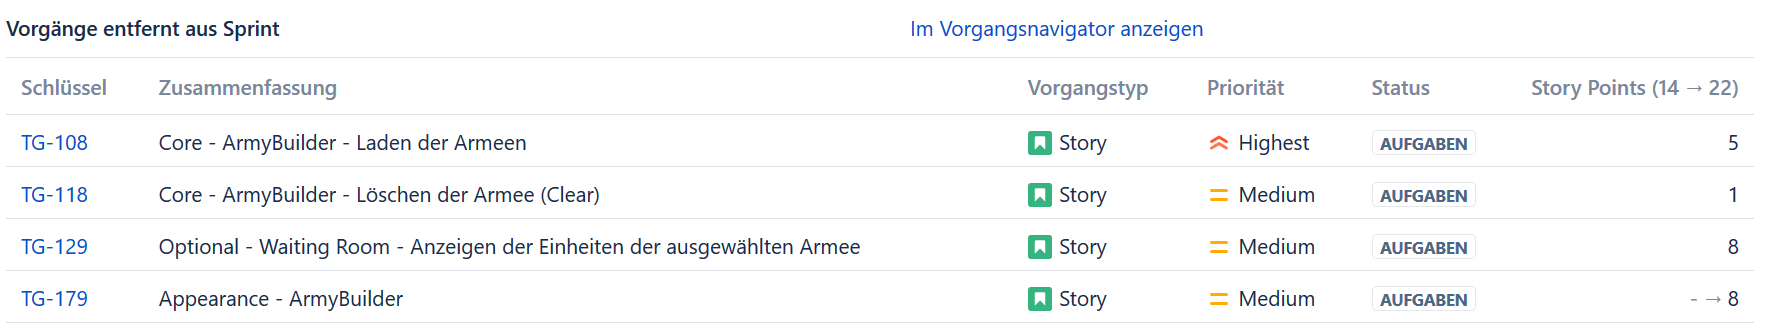
\includegraphics[width=0.8\textwidth]{Aus_dem_Sprint_Entfernte_Vorgaenge_Sprint_3.PNG}
				\caption{Entfernte Vorg�nge vom dritten Sprint}
				\label{EntfernteVorgaengeSprint3}
			\end{figure}
		
		\subsubsection{Fazit}
		Obwohl das gesetzte Ziel von 110 Story Points nicht erreicht wurde, handelt es sich dennoch um ein gutes Sprintergebnis. Es konnte ein Gro�teil der geforderten Features f�r das zweite Release bereits abgeschlossen werden. Im n�chsten Sprint kann sich deshalb mehr auf optionale Features konzentriert werden. Die aufgetretenen Probleme wurden rechtzeitig erkannt und konnten so auf ein Minimum reduziert werden. 
		
	\section{Sprint \RN{4}}
		\subsection{Sprintziel}
			Im vierten und letzten Sprint des zweiten Releases haben wir uns drei Ziele gesetzt. Als erstes sollen nat�rlich die aus dem dritten Sprint �bernommenen Aufgaben abgeschlossen werden. Der zweite Punkt ist das Einarbeiten der restlichen Features f�r das zweite Release. Obwohl ein Gro�teil der geforderten Features bereits implementiert war, fehlten jedoch noch Punkte wie das Visualisieren des Beitreten eines Spielers im Warteraum. Zuletzt wollen wir noch die Oberfl�che �berarbeiten und die Nutzererfahrung der Anwendung verbessern.
		
		\subsection{User Stories}
			Der Aufbau der User Stories wird in Abschnitt \ref{UserStoriesSprint3} erl�utert.
			
			\subsubsection{Core - ArmyBuilder - Speichern der Armeen}
			\paragraph{Ziel} Der Entwickler soll das Speichern von Armeen loakl und serverseitig implementieren.
			\paragraph{Story} Albert befindet sich in dem ArmyBuilder. Albert hat eine Armee konfiguriert. Albert klickt auf den Speichern Button. Die Armeen werden lokal und auf dem Server gespeichert.
			\paragraph{Zugeteilter Entwickler} Diese User Story bearbeitet weiterhin Tobias Klipp.
			\paragraph{Sch�tzung}
			Da das Feature von den Entwicklern als komplex eingesch�tzt wurde, erhielt es 15 Story Points.
			\paragraph{Verlauf der Entwicklung} Dieser Task wurde im vierten Sprint erneut ge�ffnet, da es noch Erweiterung gab, welche nicht zum Ende des dritten Sprints in die Quellcodebasis gezogen wurden.
			
			\subsubsection{Core - ArmyBuilder - L�schen der Armee (Clear)}
			\paragraph{Ziel} Im ArmyBuilder soll ein Button vorhanden sein mit dem man eine Armee komplett leeren kann.
			\paragraph{Story}Albert befindet sich in dem ArmyBuilder. Es ist eine Armee mit Einheiten ausgew�hlt. Albert klickt auf den Trash-Button. Alle Einheiten der ausgew�hlten Armee werden aus dieser entfernt. Es wird noch keine �nderung gespeichert.
			\paragraph{Zugeteilter Entwickler} Diese Aufgabe hat Tobias Klipp bekommen, da er das Laden und Speichern der Armee realisiert.
			\paragraph{Sch�tzung}
			Das Feature wurde auf 1 Story Points gesch�tzt.
			\paragraph{Verlauf der Entwicklung} 
			Dieses Feature wurde mit einem Story Point stark untersch�tzt. Es wurden 6h und 45min f�r die Vollendung der Story ben�tigt. Die Anforderungen f�r das L�schen waren hier spezieller, da die Armee auf dem Server gel�scht werden sollte, jedoch lokal noch vorhanden sein soll. Zudem erschwerte das Erstellen von Tests den Task.
			
			\subsubsection{Appearance - ArmyBuilder}
			\paragraph{Ziel} Es soll der AmryBuilder an das Dark Theme angepasst werden.
			\paragraph{Story} Albert befindet sich in der Lobby. Albert klickt auf den ArmyBuilder Button. Albert befindet sich nun im ArmyBuilder und es sind alle n�tigen Daten geladen und werden angezeigt. Der ArmyBuilder wird entsprechend dem Style der Mockups angezeigt.
			\paragraph{Zugeteilter Entwickler} Als Entwickler wurde Keanu St�ckrad diese Aufgabe zugewiesen.
			\paragraph{Sch�tzung}
			Das Feature wurde auf 8 Story Point gesch�tzt.
			\paragraph{Verlauf der Entwicklung} 
			Der Entwickler ben�tigte insgesamt 14h f�r die Bearbeitung der Story. In der Story wurde noch der Style des \glqq Dark Themes\grqq global angewandt, was zus�tzliche Arbeitszeit kostete. Des Weiteren mussten Tests und Mergekonflikte behoben werden, was die Bearbeitungszeit weiter in die L�nge zog.
			 
			\subsubsection{Optional - Ingame - Zoomen auf dem Spielfeld}
			\paragraph{Ziel} Es soll ein Vergr��ern und Verkleinern der Spielkarte m�glich sein.
			\paragraph{Story}Albert befindet sich in einem Spiel welches bereits gestartet ist. Es ist ein Vergr��ern-Button vorhanden. Albert klickt auf den  Verkleinern-Button. Das Spielfeld wird um eine Stufe herangezoomt.
			\paragraph{Zugeteilter Entwickler} Diese Aufgabe bearbeite Keanu St�ckrad, da er auch f�r die Implementierung des Spielfeldes verantwortlich war.
			\paragraph{Sch�tzung}
			Das Feature wurde auf 15 Story Points gesch�tzt, da es noch unklar war wie man das Zoomen realisiert werden kann.
			\paragraph{Verlauf der Entwicklung} 
			F�r diese Aufgabe wurden 5h Stunden ben�tigt. Eigentlich wurden f�r diese Story 15h angesetzt. Diese Fehleinsch�tzung resultierte daraus, dass dieses Problem f�r die Entwickler noch unbekannt war und somit eine hohe Einarbeitungszeit angesetzt wurde.
			
			\subsubsection{Core - Ingame - Spiel verlassen}
			\paragraph{Ziel} Es soll m�glich sein ein Spiel zu verlassen.
			\paragraph{Story} Albert befindet sich in einem gestartetem Spiel. Albert hat den Early Rush vermasselt. In der Ingame Scene ist ein Leave-Game-Button vorhanden. Albert klickt auf den Leave-Game-Button und verl�sst das Spiel ordnungsgem��. Albert kommt zur�ck Lobby zur�ck.
			\paragraph{Zugeteilter Entwickler} Als Entwickler wurde Keanu St�ckrad dieser Aufgabe zugeteilt.
			\paragraph{Sch�tzung}
			Das Feature wurde auf 3 Story Points gesch�tzt
			\paragraph{Verlauf der Entwicklung} 
			Es wurde insgesamt eine Arbeitszeit von 1h f�r diese Story ben�tigt. Es wurden 3h f�r f�r diese Task angesetzt. Der Entwickler konnte diese schneller abschlie�en, da bereits auf vorhande Programmlogik aufgebaut werden konnte. Die Sch�tzung auf 3h wurde auf der Grundlage getroffen, dass nicht klar, welche Aspkete beim \glqq Aufr�umen\grqq zu beachten sein werden.
			
			\subsubsection{Optional - Waiting Room - Anzeigen der Karte (Preview)}
			\paragraph{Ziel} Im Warteraum soll es eine Vorschau f�r die Karte des kommenden Spiels angezeigt werden.
			\paragraph{Story} Albert befindet sich in der Lobby. Albert tritt einem Spiel aus der Spieleliste bei. Albert wird beim Spiel angemeldt und befindet sich nun im Waiting Room. Es wird eine Vorschau f�r das kommende Spielfeld angezeigt.
			\paragraph{Zugeteilter Entwickler} Diese Story wurde von Jan M�ller bearbeitet.
			\paragraph{Sch�tzung}
			Das Feature wurde auf 3 Story Points gesch�tzt, da es auf das Anzeigen des Spielfeldes aufbaut und sich daran orientiert werden kann.
			\paragraph{Verlauf der Entwicklung} 
			Da diese Aufgabe auf dem Erstellen der Spielkarte aufbaut, konnten viele Konstrukte daraus �bernommen werden. Deshalb wurden nur 2h von den geplanten 3h ben�tigt.
			
			\subsubsection{Core - Login - Default Armeen erstellen und User auf erstellen von Armeen hinweisen}
			\paragraph{Ziel} Es sollen \glqq Defaultarmeen\grqq erstellt werden, damit der User sofort einem Spiel beitreten kann, wenn dieser das Spiel zum ersten mal spielt. Der Nutzer wird dabei auch darauf hingewiesen, das er die Armeen auch bearbeiten kann.
			\paragraph{Story} Albert befindet sich im Login Bereich und hat sich gerade registriert. Albert gibt seine Logindaten ein und meldet sich an. Albert wird erfolgreich eingeloggt. Albert befindet sich nun in der Lobby. Es gibt bereits  "Default"-Armeen und Albert wird darauf hingewiesen, dass er die Armeen �ber den Armee-Button bearbeiten kann.
			\paragraph{Zugeteilter Entwickler} Diese Story wurde von Omar Sood bearbeitet.
			\paragraph{Sch�tzung}
			Das Feature wurde auf 3 Story Points gesch�tzt.
			\paragraph{Verlauf der Entwicklung} 
			Diese Aufgabe wurde von den Entwicklern korrekt eingesch�tzt, da wir hierf�r 2h und 50 min ben�tigten.
			
			\subsubsection{Core - Lobby - Deaktivieren der JoinGame-Buttons und des Create-Game-Buttons bei keiner ausgew�hlten Armee}
			\paragraph{Ziel} Es soll nicht m�glich sein einem Spiel beizutreten, wenn man keine valide Armee ausgew�hlt hat.
			\paragraph{Story} Albert befindet sich in der Lobby. Albert hat keine Armee ausgew�hlt/ es ist keine vollst�ndige Armee vorhanden. Die "JoinGame"-Buttons der Spielliste und der Create-Game Button sind deaktiviert. Albert klick auf einen der JoinGame-Buttons. Albert bekommt einen Dialog, welcher ihm erkl�rt das er eine vollst�ndige Armee braucht, um einem Spiel beizutreten.
			\paragraph{Zugeteilter Entwickler} Diese Story wurde von Omar Sood bearbeitet.
			\paragraph{Sch�tzung}
			Das Feature wurde auf 3 Story Points gesch�tzt.
			\paragraph{Verlauf der Entwicklung} 
			Der Entwickler schloss die Aufgabe eine Stunde schneller ab als geplant.
			
			\subsubsection{Optional - ArmyBuilder - Bearbeiten der Armeeinformationen}
			\paragraph{Ziel} Im ArmyBuilder solle es die m�glichkeit geben, das Icon und den Namen der Armee zu bearbeiten.
			\paragraph{Story}Albert befindet sich im ArmyBuider. Unter der Armeeliste befindet sich ein Bearbeiten-Button. Albert hat eine Armee ausgew�hlt und klick auf den Bearbeiten-Button. Es �ffnet sich ein Dialog zum Bearbeiten der Armeeinformationen. Es ist m�glich den Namen der Armee zu bearbeiten. Es ist m�glich das Icon der Armee aus einer Liste vordefinierter Icons zu bearbeiten. Armeen werden mit einem Default Name und einem Default Icon erstellt, falls nichts n�her spezifiziert ist. Wird die auf den Speichern Button geklickt, so wird die Armee gespeichert. Wird auf den Cancel Button geklickt, so wird die View geschlossen. Es wird nichts gespeichert.
			\paragraph{Zugeteilter Entwickler} Diese Story wurde von Omar Sood bearbeitet.
			\paragraph{Sch�tzung}
			Das Feature wurde auf f�nf Story Points gesch�tzt.
			\paragraph{Verlauf der Entwicklung} 
			Der Aufwand wurde von den Entwicklern gut eingesch�tzt, da eine Arbeitszeit von 4h und 24min ben�tigt wurde.
		
			\subsubsection{Optional - ArmyBuilder - Armeeauswahl aus der Lobby �bernehmen}
			\paragraph{Ziel} Als Komfortfunktion soll es m�glich sein die ausgew�hlt Armee mit in den ArmyBuilder zu �bernehmen.
			\paragraph{Story} Albert befindet sich in der Lobby. Es ist eine Armee in der Lobby ausgew�hlt. Albert klickt auf den Armies-Button. Albert kommt in den ArmyBuilder. Im ArmyBuilder ist die Armee ausgew�hlt, welche bereits in der Lobby ausgew�hlt war.
			\paragraph{Zugeteilter Entwickler} Diese Story wurde von Omar Sood bearbeitet.
			\paragraph{Sch�tzung}
			Das Feature wurde auf 1 Story Points gesch�tzt.
			\paragraph{Verlauf der Entwicklung} 
			Der Aufwand wurde von den Entwicklern gut eingesch�tzt. Mit 1h und 18min liegen wir leicht �ber der gesch�tzten Stunde.
			
			\subsubsection{Optional - Create Game - Auto Join}
			\paragraph{Ziel} Als Komfortfunktion soll es m�glich sein, nach dem ein Spiel erstellt wurde diesem direkt beizutreten.
			\paragraph{Story} Albert befindet sich im Create Game Dialog. Albert hat eine Spielerzahl ausgew�hlt und einen Namen f�r die Armee eingegeben. Albert klickt auf "Spiel erstellen". Albert tritt dem eben erstellten Spiel automatisch bei und befindet sich jetzt im Waiting Room f�r das Spiel.
			\paragraph{Zugeteilter Entwickler} Diese Story wurde von Omar Sood bearbeitet.
			\paragraph{Sch�tzung}
			Das Feature wurde auf 1 Story Points gesch�tzt.
			\paragraph{Verlauf der Entwicklung} 
			Der Aufwand wurde von den Entwicklern perfekt eingesch�tzt. Es gab ein Punktlandung mit 1h. 
			
			\subsubsection{Appearance - Create Game - Anpassen des Style's des Create-Game-Formulars}
			\paragraph{Ziel} Das \glqq Create Game\grqq Formular soll an den aktuellen Style angepasst werden.
			\paragraph{Story} Albert befindet sich in der Lobby. Albert klickt auf den Create-Game-Button. Es �ffnet sich das CreateGame Formular. Die Buttons f�r Create Game erstrahlen im Glanze unseres Styles. (MockUps)
			\paragraph{Zugeteilter Entwickler} Diese Story wurde von Jan M�ller bearbeitet.
			\paragraph{Sch�tzung}
			Das Feature wurde auf 3 Story Points gesch�tzt.
			\paragraph{Verlauf der Entwicklung} 
			Der Aufwand wurde von den Entwicklern gut eingesch�tzt. Der Entwickler war mit 2h und 38min schneller fertig als gesch�tzt. 
			
			\subsubsection{Core - Waiting Room - Ein Spieler tritt dem Spiel bei}
			\paragraph{Ziel} Wenn ein Spieler das Spiel im Waitingroom beitritt, wird dies Visuell dargestellt.
			\paragraph{Story} Albert befindet sich im Waiting Room eines Spiels. Es befindet sich noch kein weiterer Mitspieler im Spiel. Carlie tritt dem Spiel bei. Carlie wird in einem der "Player-Kasten" angezeigt.
			\paragraph{Zugeteilter Entwickler} Diese Story wurde von Keanu St�ckrad bearbeitet. Keanu hat bereits im letzten Release an den \glqq Boxen\grqq der Spieler gearbeitet hat.
			\paragraph{Sch�tzung}
			Das Feature wurde auf 3 Story Points gesch�tzt.
			\paragraph{Verlauf der Entwicklung} 
			Der Entwickler liegt mit 3,5h leicht �ber der Sch�tzung. Dies liegt aber noch im Rahmen.
			
			\subsubsection{Core - Waiting Room - Ein Spieler verl�sst das Spiel}
			\paragraph{Ziel} Wenn ein Spieler das Spiel im Waitingroom verl�sst, wird dies Visuell dargestellt.
			\paragraph{Story} Albert befindet sich im Waiting Room von Albert's Spiel. Carlie befindet sich ebenfalls in Albert's Spiel. Carlie hat noch ein Date und kann deshalb nicht mitspielen. Carlie verl�sst das Spiel. Carlie wird aus seinem "Player-Kasten" entfernt. Alle anderen Mitspieler bleiben in Ihren "Player-Kasten".
			\paragraph{Zugeteilter Entwickler} Diese Story wurde von Keanu St�ckrad bearbeitet. Keanu hat bereits im letzten Release an den \glqq Boxen\grqq der Spieler gearbeitet und den auch das Beitreten eines Spielers bearbeitet, war er die beste Wahl f�r diese Aufgabe.
			\paragraph{Sch�tzung}
			Das Feature wurde auf 2 Story Points gesch�tzt.
			\paragraph{Verlauf der Entwicklung} 
			Da der Entwickler bereits Erfahrung mit der Problematik hatte, wurde diese Aufgabe mit 1h schneller als gesch�tzt abgeschlossen.
			
			\subsubsection{Optional - Waiting Room - "Player-Kasten" wird mit der Spielerfarbe dargestellt}
			\paragraph{Ziel} Spieler im Waiting Room werden mit ihren entsprechenden Farben dargestellt.
			\paragraph{Story} Albert befindet sich in der Lobby. Albert tritt Carlie's Game bei. Albert befindet sich nun in Carlie's Game Waiting Room. Die "Player-Kasten" werden mit den Farben des jeweiligen Spielers dargestellt.
			\paragraph{Zugeteilter Entwickler} Diese Story wurde von Keanu St�ckrad bearbeitet. Keanu hat bereits im letzten Release an den \glqq Boxen\grqq der Spieler gearbeitet und auch das Beitreten und Verlassen bearbeitet.
			\paragraph{Sch�tzung}
			Das Feature wurde auf 2 Story Points gesch�tzt.
			\paragraph{Verlauf der Entwicklung} 
			Da der Entwickler bereits Erfahrung mit der Problematik hatte, wurde diese Aufgabe mit 1h schneller als gesch�tzt abgeschlossen.
			
			\subsubsection{Appearance - Alerts}
			\paragraph{Ziel} Die Popup-Meldungen sollten dem \glqq Dark Theme\grqq angepasst werden.
			\paragraph{Story} Albert befindet sich in der Lobby. Albert klickt auf Logout. Es �ffnet sich ein Overlay, was die Alerts ersetzt. Das Overlay erstrahlt im Glanze unseres Styles. Es sollen alle Alerts durch die Overlays erstezt werden.
			\paragraph{Zugeteilter Entwickler} Diese Story wurde von Jan M�ller bearbeitet. 
			\paragraph{Sch�tzung}
			Das Feature wurde auf 3 Story Points gesch�tzt.
			\paragraph{Verlauf der Entwicklung} 
			f�r Bearbeitung dieser Aufgabe wurden ca. 9h ben�tigt. Der Entwickler realisierte eine entsprechende Funktion um einfach und individuell Meldungen generieren zu k�nnen. Dies wurde durch den Scrum Master best�tigt, da wir dadurch im sp�teren Entwicklungsverlauf Zeit und Ressourcen sparen k�nnen.
			
			\subsubsection{Core - ArmyBuilder - "CanAttack" �bersicht}
			\paragraph{Ziel} Die Detailansicht soll in um eine \glqq Can Attack\grqq-Ansicht erweitert werden.
			\paragraph{Story} Albert befindet sich im ArmyBuilder. Albert w�hlt eine Einheit aus der "Unit Selection" aus. Es wird die Detail View zur Einheit angezeigt. In der Detail View ist eine �bersicht zu "Can Attack" vorhanden.
			\paragraph{Zugeteilter Entwickler} Diese Story wurde von Omar Sood bearbeitet. Die Aufgabe wurde Omar zugeteilt, da dieser die Detailansicht schon in einer vorhergehen Story realisiert hat.
			\paragraph{Sch�tzung}
			Das Feature wurde auf f�nf Story Points gesch�tzt.
			\paragraph{Verlauf der Entwicklung} 
			Da der Entwickler bereits Erfahrungen mit der Detailansicht hat konnte die Aufgabe mit 3h und 49min schneller abgeschlossen werden.
			
			\subsubsection{Optional - ArmyBuilder- Indikator ob Speichern n�tig ist und Aktivieren des Save Buttons}
			\paragraph{Ziel} Die Detailansicht soll in um eine \glqq Can Attack\grqq-Ansicht erweitert werden.
			\paragraph{Story} Albert befindet sich in der Lobby. Albert hat noch keine �nderungen an den Armeen vorgenommen. Der Indikator zum Speichern ist Grau. Der Save-Button ist Disabled. Albert f�gt eine Einheit seiner Armee hinzu. Der Indikator zum Speicher hat die Farbe von Primary Two. Der Save-Button ist Enabled.
			\paragraph{Zugeteilter Entwickler} Diese Story wurde von Omar Sood bearbeitet. Die Aufgabe wurde Omar zugeteilt, da dieser schon viel im ArmyBuilder implementiert hat.
			\paragraph{Sch�tzung}
			Das Feature wurde auf f�nf Story Points gesch�tzt.
			\paragraph{Verlauf der Entwicklung} 
			Der Entwickler war mit 2h und 42min doppelt so schnell wie gesch�tzt. Die Story wurde im positiven Sinne von den Entwicklern �bersch�tzt.
			\subsubsection{Core - ArmyBuilder - Laden der Armeen}
			\paragraph{Ziel} Die gespeicherten Armeen sollen Lokal und vom Server geladen werden.
			\paragraph{Story} Albert befindet sich im Login Bereich. Albert loggt sich erfolgreich beim Spiel ein. Die Lokal/auf dem Server gespeicherten Armeen werden geladen. Albert befindet sich in der Lobby, die geladenen Armeen werden in der Armeenliste angezeigt.
			\paragraph{Zugeteilter Entwickler} Diese Story wurde von Tobias Klipp bearbeitet. Die Aufgabe wurde Tobias zugeteilt, da dieser bereits das Laden implementiert hat und somit bereits Erfahrung f�r diese Aufgabe besitzt.
			\paragraph{Sch�tzung}
			Das Feature wurde auf f�nf Story Points gesch�tzt.
			\paragraph{Verlauf der Entwicklung} 
			Die Story ben�tigte eine Arbeitszeit von insgesamt 16h und 16min. Die Schwierigkeit bei der Implementierung war, dass die gespeicherten Armeen auf dem Server und Lokal zusammengef�hrt werden. Der Entwickler hatte auch Probleme damit, das Feature umzusetzen, da die Kommunikation mit dem Server noch neu war und er sich in die Thematik einarbeiten musste.
			\subsubsection{Optional - Chat - Anzeigen das eine Nachricht angekommen ist}
			\paragraph{Ziel} Der Nutzer soll im Chat darauf aufmerksam gemacht werden, dass er eine neue Nachricht erhalten hat, in einem inaktiven Chat.
			\paragraph{Story}Albert befindet sich in der Lobby. Albert hat mit Carlie gechattet und wechselt in den General-Chat. Carlie schickt eine Nachricht an Albert. Der Chat-Tab von Carlie wird bei Albert hervorgehoben, so das Albert erkennt, dass eine neuen Nachricht angekommen ist.
			\paragraph{Zugeteilter Entwickler} Die Story wurde Jan M�ller zugeteilt, da diese bereits f�r die Implementierung des Chats zust�ndig war. 
			\paragraph{Sch�tzung}
			Das Feature wurde auf 3 Story Points gesch�tzt.
			\paragraph{Verlauf der Entwicklung} 
			Der Entwickler konnte die Story mit 1h 40m schneller abSchlie�en als erwartet.  
			\subsubsection{Optional - ArmyBuilder - Bearbeiten der Armeeinformationen}
			\paragraph{Ziel} Der Nutzer soll im Chat darauf aufmerksam gemacht werden, dass er eine neue Nachricht erhalten hat, in einem inaktiven Chat.
			\paragraph{Story} Albert befindet sich im ArmyBuider. Unter der Armeeliste befindet sich ein Bearbeiten-Button. Albert hat eine Armee ausgew�hlt und klick auf den Bearbeiten-Button. Es �ffnet sich ein Dialog zum Bearbeiten der Armeeinformationen. Es ist m�glich den Namen der Armee zu bearbeiten. Es ist m�glich das Icon der Armee aus einer Liste vordefinierter Icons zu bearbeiten. Armeen werden mit einem Default Name und einem Default Icon erstellt, falls nichts n�her spezifiziert ist. Wird die auf den Speichern Button geklickt, so wird die Armee gespeichert. Wird auf den Cancel-Button geklickt, so wird die View geschlossen. Es wird nichts gespeichert.
			\paragraph{Zugeteilter Entwickler} Die Story wurde Omar Sood zugeteilt.
			\paragraph{Sch�tzung}
			Das Feature wurde auf f�nf Story Points gesch�tzt.
			\paragraph{Verlauf der Entwicklung} 
			Mit 4h 24m war der Entwickler schneller als geplant.  
			\subsubsection{Core - ArmyBuilder - Autosave der Armeen bei verlassen des ArmyBuilders}
			\paragraph{Ziel} �nderungen an den Armeen sollen automatisch nach verlassen des ArmyBuilders gespeichert werden.
			\paragraph{Story} Albert befindet sich im ArmyBuilder. Albert hat ein paar Armeen erstellt und bearbeitet. Albert hat seine �nderungen noch nicht gespeichert. Albert klickt auf den "zur�ck"-Button. Es werden alle Armeen gespeichert. Albert wird in die Lobby zur�ck navigiert.
			\paragraph{Zugeteilter Entwickler} Die Story wurde Tobias Klipp zugeteilt.
			\paragraph{Sch�tzung}
			Das Feature wurde auf 1 Story Points gesch�tzt.
			\paragraph{Verlauf der Entwicklung} 
			Der Entwickler ben�tigte 15 Minuten, um die Aufgabe abzuSchlie�en. Die Aufgabe wurde schneller abschlossen als erwartet.
			\subsubsection{Core - ArmyBuilder - Can Attack �bersicht}
			\paragraph{Ziel} In der Detailansicht einer Einheit, soll es eine Can Attack �bersicht geben.
			\paragraph{Story} Albert befindet sich im ArmyBuilder. Albert hat ein paar Armeen erstellt und bearbeitet. Albert hat seine �nderungen noch nicht gespeichert. Albert klickt auf den Zur�ck-Button. Es werden alle Armeen gespeichert. Albert wird in die Lobby zur�ck navigiert.
			\paragraph{Zugeteilter Entwickler} Die Story wurde Omar Sood zugeteilt. Omar hatte bereits die Detailansicht f�r Einheit implementiert, womit er die meiste Erfahrung in diesen Bereich hat.
			\paragraph{Sch�tzung}
			Das Feature wurde auf f�nf Story Points gesch�tzt.
			\paragraph{Verlauf der Entwicklung} 
			Der Arbeitsaufwand f�r diese Story belief sich auf 3h und 49m. Damit war der Entwickler schneller als geplant.
			\subsubsection{Optional - ArmyBuilder- Indikator ob Speichern n�tig ist und Aktivieren des Save Buttons}
			\paragraph{Ziel} Im ArmyBuilder soll es ein visuelles Feedback geben, ob aktuellen Armeen gespeichert sind.
			\paragraph{Story} Albert befindet sich in der Lobby. Albert hat noch keine �nderungen an den Armeen vorgenommen. Der Indikator zum Speichern ist Grau. Der Save-Button ist Disabled. Albert f�gt eine Einheit seiner Armee hinzu. Der Indikator zum Speicher hat die Farbe von Primary Two. Der Save-Button ist Enabled.
			\paragraph{Zugeteilter Entwickler} Die Story wurde Omar Sood zugeteilt.
			\paragraph{Sch�tzung}
			Das Feature wurde auf f�nf Story Points gesch�tzt.
			\paragraph{Verlauf der Entwicklung} 
			Die Story wurde mit 2h und 42 in der H�lfte der geplanten Zeit erledigt.
			\subsubsection{Optional - Waiting Room - Anzeigen der Einheiten der ausgew�hlten Armee}
			\paragraph{Story} Albert befindet sich in der Lobby und hat eine Armee ausgew�hlt. Albert tritt einem Spiel bei. Albert wird erfolgreich beim Spiel angemeldet und befindet sich im Waiting Room des Spiels. Entsprechend dem MockUp werden die Einheiten der ausgew�hlten Armee angezeigt.
			\paragraph{Sch�tzung}
			Das Feature wurde auf 8 Story Points gesch�tzt.
			\paragraph{Verlauf der Entwicklung} 
			Die Story wurde nicht in Sprint 4 begonnen und wird auch nicht in den n�chsten Sprint �bernommen werden.
			\subsubsection{Optional - Lobby - Anzeigen der Einheiten einer Armee}
			\paragraph{Story} Albert befindet sich im ArmyBuilder. Es sind Armeen vorhanden. Albert hovert �ber eine Armee. Es erscheint ein Overlay, in welchem die Einheiten der Armeen sehen kann.
			\paragraph{Sch�tzung}
			Das Feature wurde auf f�nf Story Points gesch�tzt.
			\paragraph{Verlauf der Entwicklung} 
			Die Story wurde nicht in Sprint 4 begonnen und wird auch nicht in den n�chsten Sprint �bernommen werden.
			\subsubsection{Optional - ArmyBuilder- Notifiaction f�r das Speichern der Armee und Waiting Animation.}
			\paragraph{Story} Albert befindet sich in der Lobby. Albert hat eine Armee bearbeitet. Albert klickt auf den Speicher Button. Der Speicherprozess beginnt. Es wird eine Warteanimation angezeigt. Der Speicherprozess endet. Es wird eine Notification angezeigt mit dem Status des Speicherns.
			\paragraph{Sch�tzung}
			Das Feature wurde auf f�nf Story Points gesch�tzt.
			\paragraph{Verlauf der Entwicklung} 
			Da der Speicherprozess nur sehr wenig Zeit ben�tigt, ist das Anzeigen eines Ladebalkens nicht n�tig. Die Story wird deshalb nicht umgesetzt.
			\subsubsection{Core - ArmyBuilder - Lokaler Speicherort f�r Armeen}
			\paragraph{Ziel} Der Speicherort der Armeen soll lokal an die Betriebssysteme Windows, Unix und MacOs angepasst werden. 
			\paragraph{Story} Albert befindet sich im ArmyBuilder. Albert klickt auf Speichern. Die Armeen werden lokal gespeichert an einem von uns definierten betriebssystemabh�ngigen Speicherort.
			z.B. Windows: AppData 
			\paragraph{Sch�tzung}
			Das Feature wurde auf f�nf Story Points gesch�tzt.
			\paragraph{Verlauf der Entwicklung} 
			Das Feature konnte in 30 Minuten fertig gestellt werden. Die Story wurde erst im 5. Sprint vom Entwickler geschlossen. Die Funktionalität war jedoch bereits im zweiten Release vorhanden.
			\subsection{Tasks}
			Auch im vierten Sprint wurden einzelne Tasks erstellt, die keiner User Story zugeordnet waren. Da keine Story Punkte auf Tasks geschätzt werden konnten, wurden lediglich Zeitschätzungen eingetragen.
			\subsubsection{Task - SceneManger überarbeiten}
			\paragraph{Ziel} Der Szenenwechsel sollte soweit überarbeitet werden, dass bestimmte Szenenwechsel, z. B. vom der Lobby zum ArmyBuilder, möglich sind, ohne dass die Controller terminiert werden und damit die Websocketverbindung zum Server geschlossen wird.
			\paragraph{Zugeteilter Entwickler} Jan Müller bearbeitete diesen Task.
			\paragraph{Schätzung}
			Dieser Task wurde auf acht Stunden geschätzt.
			\paragraph{Verlauf der Entwicklung} Da der Entwickler auf der Arbeit in einer anderen User Story aufbauen konnte, benötigte er mit 1h und 35 Minuten deutlich weniger Zeit.
			\subsubsection{Task - Neues Musikstück einpflegen}
			\paragraph{Ziel} Das bisher verwendete Musikstück sollte durch ein anderes 8-Bit Musikstück ersetzt werden.
			\paragraph{Zugeteilter Entwickler} Dieser Task wurde von Keanu Stückrad bearbeitet.
			\paragraph{Schätzung}
			Für die Implementierung wurde eine Stunde geschätzt.
			\paragraph{Verlauf der Entwicklung} Der Task konnte nach einer Stunde vom Entwickler abgeschlossen werden.
			\subsubsection{Task - Spiel verlassen}
			\paragraph{Ziel} Das Verlassen des Spiel sollte dahingehend verändert werden, dass beim Verlassen der Spielwebsocket nicht mehr vom Client geschlossen wird. Stattdessen soll unsere Applikation nach der leaveGame-Nachricht an den Server, auf das Schließen des Websockets durch den Server warten.
			\paragraph{Zugeteilter Entwickler} Jan Müller bearbeitete diesen Task.
			\paragraph{Schätzung}
			Es wurden fünf Stunden für diesen Task geschätzt.
			\paragraph{Verlauf der Entwicklung} Mit einer Stunde wurde der Task deutlicher schneller als geschätzt abgeschlossen.
			\subsubsection{Task - NullPointer Exception - Spielbeitritt}
			\paragraph{Ziel} Wenn bei einem Spielbetritt der Server mit einer NullPointerException reagiert, soll diese in unserer Applikation aufgefangen werden. Es soll ein Szenenwechsel in die Lobby erfolgen und dem Nutzer soll eine Fehlermeldung angezeigt werden.
			\paragraph{Zugeteilter Entwickler} Dieser Task wurde Jan Müller zugewiesen.
			\paragraph{Schätzung} Der Task wurde auf drei Stunden geschätzt.
			\paragraph{Verlauf der Entwicklung} Der Entwickler benötigte eine Stunde um diesen Taks abzuschließen.
			\subsubsection{Task - Reaktion auf 503 vom Server}
			\paragraph{Ziel} Wenn der Spieler aufgrund von Inaktivität mit einer 503 Response ausgeloggt wird, soll der Nutzer wieder zum Login geleitet werden und eine Fehlermeldung soll angezeigt werden.
			\paragraph{Zugeteilter Entwickler} Jan Müller bearbeitete diesen Task.
			\paragraph{Schätzung} Die Schätzung für diesen Task betrug eine Stunde.
			\paragraph{Verlauf der Entwicklung} Tatsächlich benötigte der Entwickler eine Stunde und 30 Minuten für diesen Task.
			\subsubsection{Task - ArmyManager Lore}
			\paragraph{Ziel} Die Einheiten im ArmyBuilder sollten neue Bilder sowie Beschreibungstexte erhalten, die in einem Fantasyuniversum angesiedelt sind.
			\paragraph{Zugeteilter Entwickler} Dieser Task wurde Omar Sood zugeordnet.
			\paragraph{Verlauf der Entwicklung} Für diesen Task benötigte der Entwickler 10 Stunden und 40 Minuten.
			\subsubsection{Task - Zwischenrelease v0.3}
			\paragraph{Ziel} Zur Vorbereitung der Abgabe auf 
			\paragraph{Zugeteilter Entwickler} Dieser Task wurde Jan Müller zugewiesen.
			\paragraph{Schätzung} Der Task wurde auf drei Stunden geschätzt.
			\paragraph{Verlauf der Entwicklung} Der Entwickler benötigte eine Stunde um diesen Taks abzuschließen.
			\newpage
			
			\subsection{Zeitübersicht}
			\begin{center}
				\begin{longtable}{p{6cm} c c c c }
					
					User Story	& Story Points & Soll Zeit & Ist Zeit & Entwickler\\
					\toprule
					\endhead
					Core - ArmyBuilder - Laden der Armeen & 5 & 5h & 16h 16min & Tobias Klipp \\ \hline 
					
					Core - ArmyBuilder - Speichern der Armeen & 13 & 13h & 34h 45min & Tobias Klipp \\ \hline
					
					Core - ArmyBuilder - L�schen der Armee (Clear) & 1 & 1h & 6h 45m & Tobias Klipp \\ \hline
					
					Optional - Waiting Room - Anzeigen der Karte (Preview) & 3 & 3h & 2h 2m& Jan M�ller \\ \hline
					
					Optional - Ingame - Zoomen auf dem Spielfeld & 13 & 13h & 7h & Keanu St�ckrad \\ \hline
					
					Core - Ingame - Spiel verlassen & 3 & 3h & 1h & Keanu St�ckrad\\ \hline
					
					Appearance - ArmyBuilder & 8 & 8h & 14h & Keanu St�ckrad\\ \hline
					
					Core - Login - Default Armeen erstellen und User auf erstellen von Armeen hinweisen & 3 & 3h & 4h 8m & Omar Sood\\ \hline
					
					Core - Lobby - Deaktivieren der JoinGame-Buttons und des Create-Game-Buttons bei keiner ausgew�hlten Armee & 3 & 3h & 2h & Omar Sood\\ \hline
					
					Optional - Chat - Anzeigen das eine Nachricht angekommen ist  & 3 & 3h & 1h 40m & Omar Sood\\ \hline
					
					Optional - ArmyBuilder - Bearbeiten der Armeeinformationen & 5 & 5h & 4h 24m & Omar Sood\\ \hline
					
					Optional - ArmyBuilder - Armeeauswahl aus der Lobby �bernehmen & 1 & 1h & 1h 18m & Omar Sood\\ \hline
					
					Optional - Create Game - Auto Join & 1 & 1h & 1h 16m & Omar Sood\\ \hline
					
					Appearance - Create Game - Anpassen des Style's des Create-Game-Formulars & 3 & 3h & 2h 38m & Jan M�ller\\ \hline
					
					Core - Waiting Room - Ein Spieler tritt dem Spiel bei & 3 & 3h & 3h 30m & Keanu St�ckrad\\ \hline
					
					Core - Waiting Room - Ein Spieler verl�sst das Spiel & 2 & 2h & 1h & Keanu St�ckrad \\ \hline
					
					Optional - Waiting Room - "Player-Kasten" \ wird mit der Spielerfarbe dargestellt & 2 & 2h & 1h & Keanu St�ckrad\\ \hline
					
					Core - ArmyBuilder - Autosave der Armeen bei verlassen des ArmyBuilders & 1 & 1h & 15m & Tobias Klipp\\
					
					Appearance - Alerts & 3 & 3h & 8h 55m & Omar Sood \\ \hline
					
					Core - ArmyBuilder - \glqq CanAttack\grqq �bersicht & 5 & 5h & 3h 49m & Omar Sood \\ \hline
					
					Appearance - Alerts & 3 & 3h & 8h 55m & Jan M�ller \\ \hline
					
					Optional - ArmyBuilder- Indikator ob Speichern n�tig ist und Aktivieren des Save Buttons & 5 & 5h & 2h 42m & Omar Sood\\
					\caption{�bersicht der Zeiten f�r den 4. Sprint} \\
				\end{longtable}
			\end{center}
			
		\subsection{Analyse des 4. Sprint}
			Der 4. Sprint wurde am 07.07.2019 abgeschlossen. Es wurden insgesamt 86 von 109 Story Points abgeschlossen. Es wurden alle KernFunktionalit�ten und viele optionale Features umgesetzt. Im folgenden wird noch einmal der Verlauf des Sprints Analysiert und eine �bersicht �ber die nicht abgeschlossenen User Stories gegeben. 
		
			\subsubsection{Burndown-Diagramm}
			In \Abb{BurndownSprint4} ist das Burndown-Diagramm f�r Sprint 4 zusehen. Insgesamt ist der Verlauf gesehen Verl�uft der Burndown-Graph so wie vorgesehen. Es gibt jedoch zwei Ausl�ufer. Der erste findet am Anfang des Sprints statt, wo am 25.06�6.2019 die Anzahl der Story Points ansteigt. Die Ursache daf�r ist, dass der Scrum Master eine abgeschlossene Story erneut ge�ffnet hatte, damit ein Entwickler seine Zeiten nachtragen kann. Die Ursache ist als lediglich ein organisatorischer Fehler. Der letzte Ausrei�er ist das Ende des Sprints, da die Kurve nicht auf Null Story Points f�llt. Es waren also noch User Stories nicht abgeschlossen. Das hatte zwei Gr�nde. Zum Einem hatte die Entwickler bereits Ihre geforderte Arbeitszeit absolviert und es handelte sich nur noch um optionale Tasks, weshalb deren Bearbeitung nicht als zwingend notwendig angesehen wurde. Zum andren haben sich der Product Owner und der Scrum Master bei den Aufgaben f�r den vierten Sprint versch�tzt und deshalb zu viele Aufgaben generiert.
			\begin{figure}[H] 
				\centering
				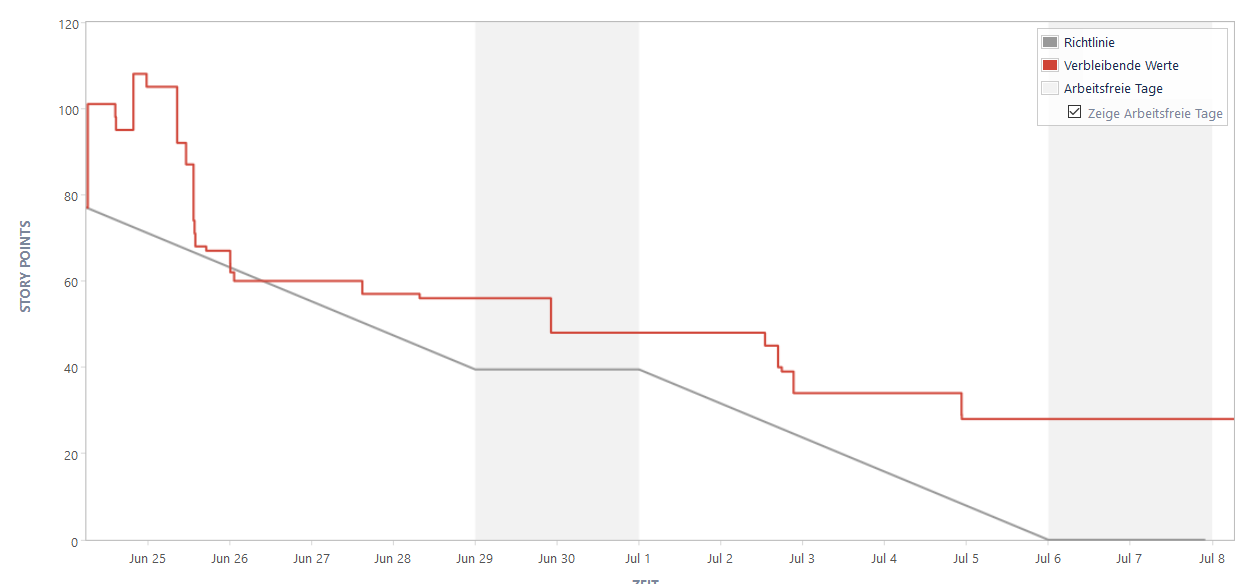
\includegraphics[width=1\textwidth]{BurndownChart_Sprint4.PNG}
				\caption{Burndown-Diagramm des Sprint 4}
				\label{BurndownSprint4}
			\end{figure}

			\subsubsection{Abgeschlossene Vorg�nge}	
			In \Abb{AbgeschlosseneVorgaengeSprint4} sind die abgeschlossenen Vorg�nge f�r den 4. Sprint zu sehen. Es konnten alle geforderten Features f�r das zweite Release umgesetzt werden. Es konnten noch folgende optionale Features umgesetzt werden:
			\begin{itemize}
				\item eine Kartenvorschau im Warteraum
				\item Zoomen auf dem Spielfeld
				\item Benachrichtigung f�r ungelesene Nachrichten
				\item Bearbeiten von Armeeinformationen
				\item Im Warteraum werden die Spieler mit entsprechender Farbe dargestellt
				\item ein Indikator f�r das Speichern im Armeemanager
			\end{itemize}
			\begin{figure}[H] 
				\centering
				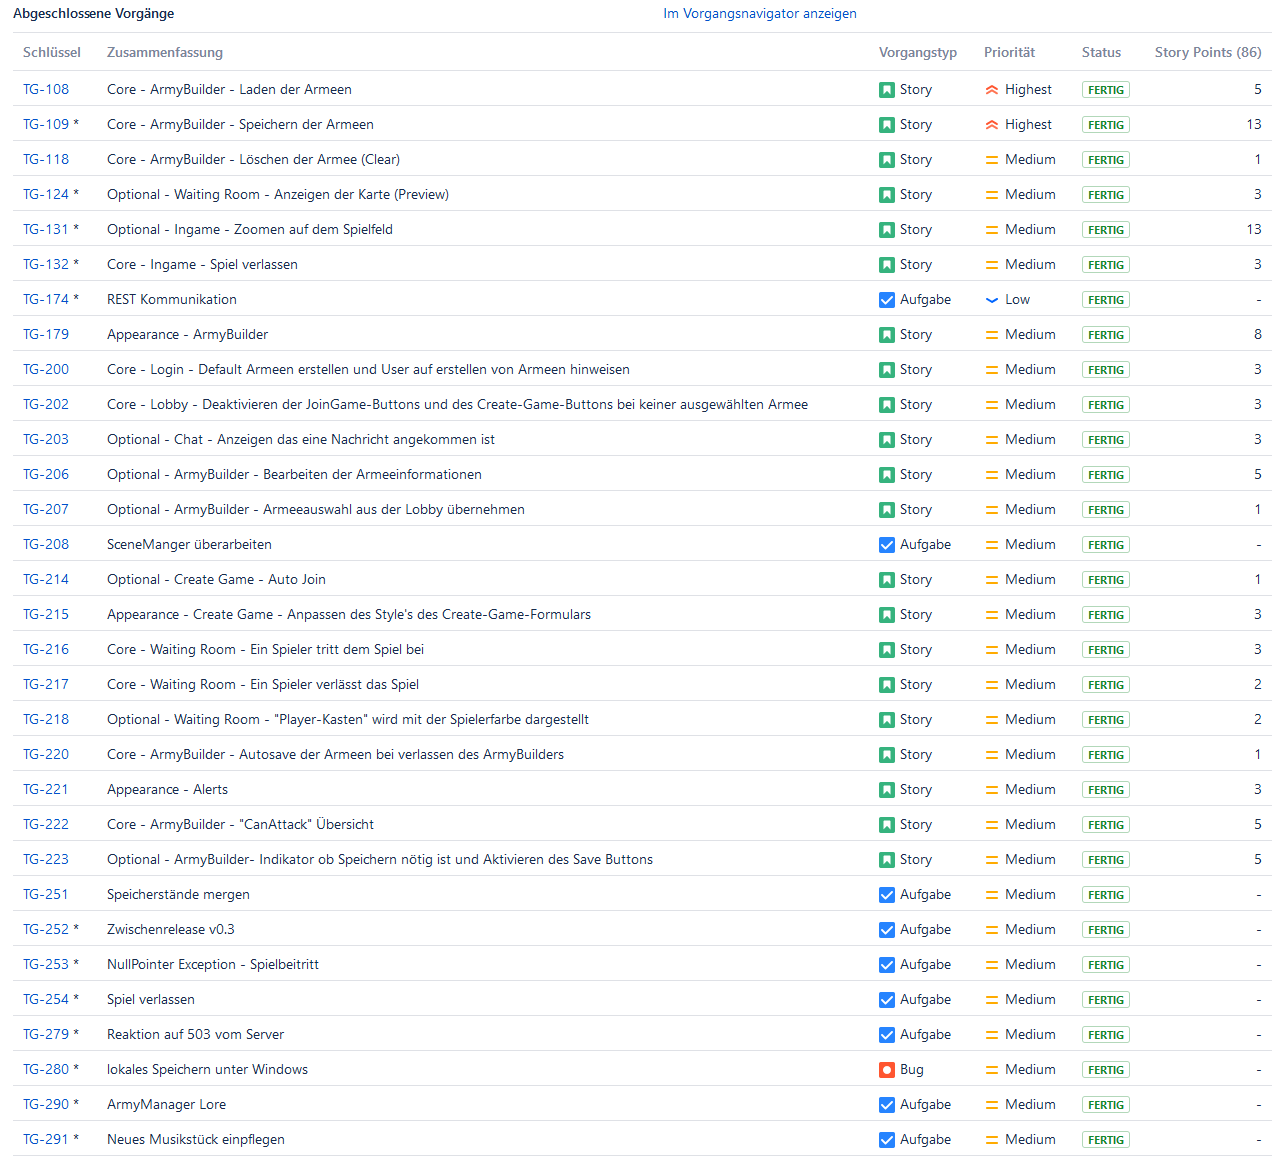
\includegraphics[width=1\textwidth]{Abschlossene_Vorgaenge_Sprint_4.png}
				\caption{Abgeschlossene Vorg�nge in Sprint 4}
				\label{AbgeschlosseneVorgaengeSprint4}
			\end{figure}
			
			\subsubsection{Nicht abgeschlossene Vorg�nge}
			In Sprint 4 wurden insgesamt 23 Story Points nicht umgesetzt. Unter diesen befindet sich kein Kernfeature. Die nicht abgeschlossenen User Stories werden nun im Nachfolgenden betrachtet. EIne �bersicht �ber diese diese ist in \Abb{NichtAbgeschlosseneVorgaengeSprint4} zu finden.
			
				\paragraph{Optional - Waiting Room - Anzeigen der Einheiten der ausgew�hlten Armee}
				\label{OWaitingRoomAnzeigenEinheiten}
				In dieser Story sollten die Einheiten der ausgewahlten Armee im Warteraum angezeigt werden. Es stellte sich jedoch heraus, dass dies im n�chsten Sprint wieder verworfen werden m�sste, weshalb andere Aufgaben priorisiert wurden, um Arbeitszeit nicht in unn�tige Features zu stecken. Diese Story wird im f�nften Sprint nicht weitergef�hrt.
				
				\paragraph{Optional - Lobby- Anzeigen der Einheiten einer Armee}
				Ziel dieser Story war es die Einheiten der Armeen in der Lobby anzuzeigen. Auch diese Story wurde verworfen. Die Gr�nde daf�r waren die selben wie in \ref{OWaitingRoomAnzeigenEinheiten}. Die Story wird im f�nften Sprint nicht weitergef�hrt.
				
				\paragraph{Optional - ArmyBuilder - Notification f�r das Speichern der Armee und Waiting Animation}
				Im Armeemanager sollte w�hrend des Speichervorgangs ein Fortschrittsbalken angezeigt werden und eine Benachrichtigung f�r das erfolgreiche Speichern erstellt werden. Da der Speichervorgang jedoch immer sehr schnell abgeschlossen wurde, ist das Anzeigen der eben genanten Visualisierungen verworfen wurden.
				
				\paragraph{Core - ArmyBuilder - Lokaler Speicherort f�r Armeen}
				Dieses Feature ist bereits im zweiten Release enthalten. Es wird noch unter den nicht abgeschlossenen Vorg�ngen aufgef�hrt, weil die Vorgang im Jira nicht rechtzeitig abgeschlossen wurde.
			
				
			\begin{figure}[H] 
				\centering
				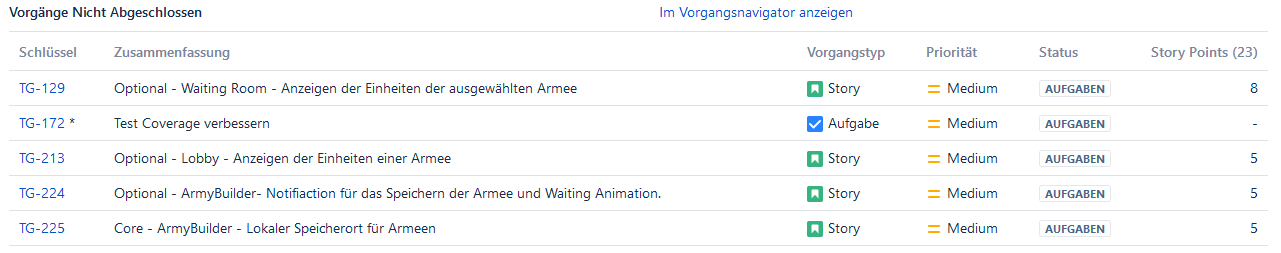
\includegraphics[width=1\textwidth]{Nicht_Abgeschlossene_Vorgaenge_Sprint_4.PNG}
				\caption{Nicht Abgeschlossene Vorg�nge in Sprint 4}
				\label{NichtAbgeschlosseneVorgaengeSprint4}
			\end{figure}
		
			\subsubsection{Fazit}
			Wir sehen den Sprint 4 als erfolgreich an, da alle restlichen KernFunktionalit�ten und viele weitere optionale Features abgeschlossen werden konnten. Das von uns gesetzte Sprintziel konnte somit erreicht werden. Von den 23 �ber gebliebenen Story Points wurden 18 verworfen, der Product Owner und Scrum Master haben bei diesen �bersehen sie aus dem Jira zu entfernen. Die �brigen f�nf Story Points wurden im Jira nur nicht diesem Sprint zugeordnet, da der Entwickler die Aufgabe zu sp�t abgeschlossen hat. Somit bleiben am Ende auch keine Aufgaben �ber, womit die Sch�tzung f�r den 4. Sprinte eingehalten werden konnte.
			
			\paragraph{Code Coverage}
			AbSchlie�end sei noch zu erw�hnen, dass auch diesen Sprint die Quellcodeabdeckung weiter ausgebaut werden konnte. In \Abb{CodeCoverageReleaseTwo} ist eine �bersicht �ber die finale Code Coverage zum Ende von Release 2. Wir erreichen eine Abdeckung von insgesamt 76\%, womit die Anforderung von 60\% CO Coverage erf�llt ist.
			
			\begin{figure}[H] 
				\centering
				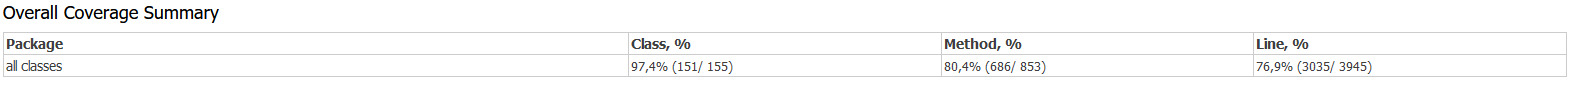
\includegraphics[width=1\textwidth]{Coverage_Sprint_4.PNG}
				\caption{Quellcodeabdeckung Release 2}
				\label{CodeCoverageReleaseTwo}
			\end{figure}
			
			\section{Abschluss des 2. Releases}
			Das zweite Release wurde am 07.07.2019 abgeschlossen. Im nachfolgenden Teil werden nun die Mockups mit der Implementierung verglichen. Dabei wir auf Unterschiede und nicht realisierte Features eingegangen und die Ursachen erl�utert.
			
			\subsection{Der Armeemanager}
			Zu Begin des Release wurde folgende Anforderungen an den Armeemanager gestellt:
			\begin{itemize}
				\item Erstellen und Konfigurieren von Armeen
				\item Armeen d�rfen maximal 10 Einheiten enthalten
				\item Speichern soll Lokal und auf dem Server erfolgen
				\item Speichern von mindestens 3 Armeen
			\end{itemize}
			Diese Anforderungen wurden zum Ende des zweiten Releases abgedeckt. Die Armeen werden automatisch erstellt und es werden dem Nutzer 7 zu Konfiguration zur Verf�gung gestellt. Ver�ndert werden k�nnen die Armeen �ber die \glqq +\grqq \ und \glqq -\grqq \ Buttons. Gespeichert werden kann �ber den Speichern Button. Die 7 Armeen werden dabei lokal und auf dem Server gespeichert. Die Umsetzung war dabei in 3 Kernbereiche aufgeteilt. Diese werden in \Abb{MockUpArmeemanager} gezeigt.
			\begin{itemize}
				\item Der Einheitenauswahl mit Detailansicht
				\item Der Armee�bersicht
				\item Der Armeeauswahl
			\end{itemize} 
		
			\begin{figure}[H] 
				\centering
				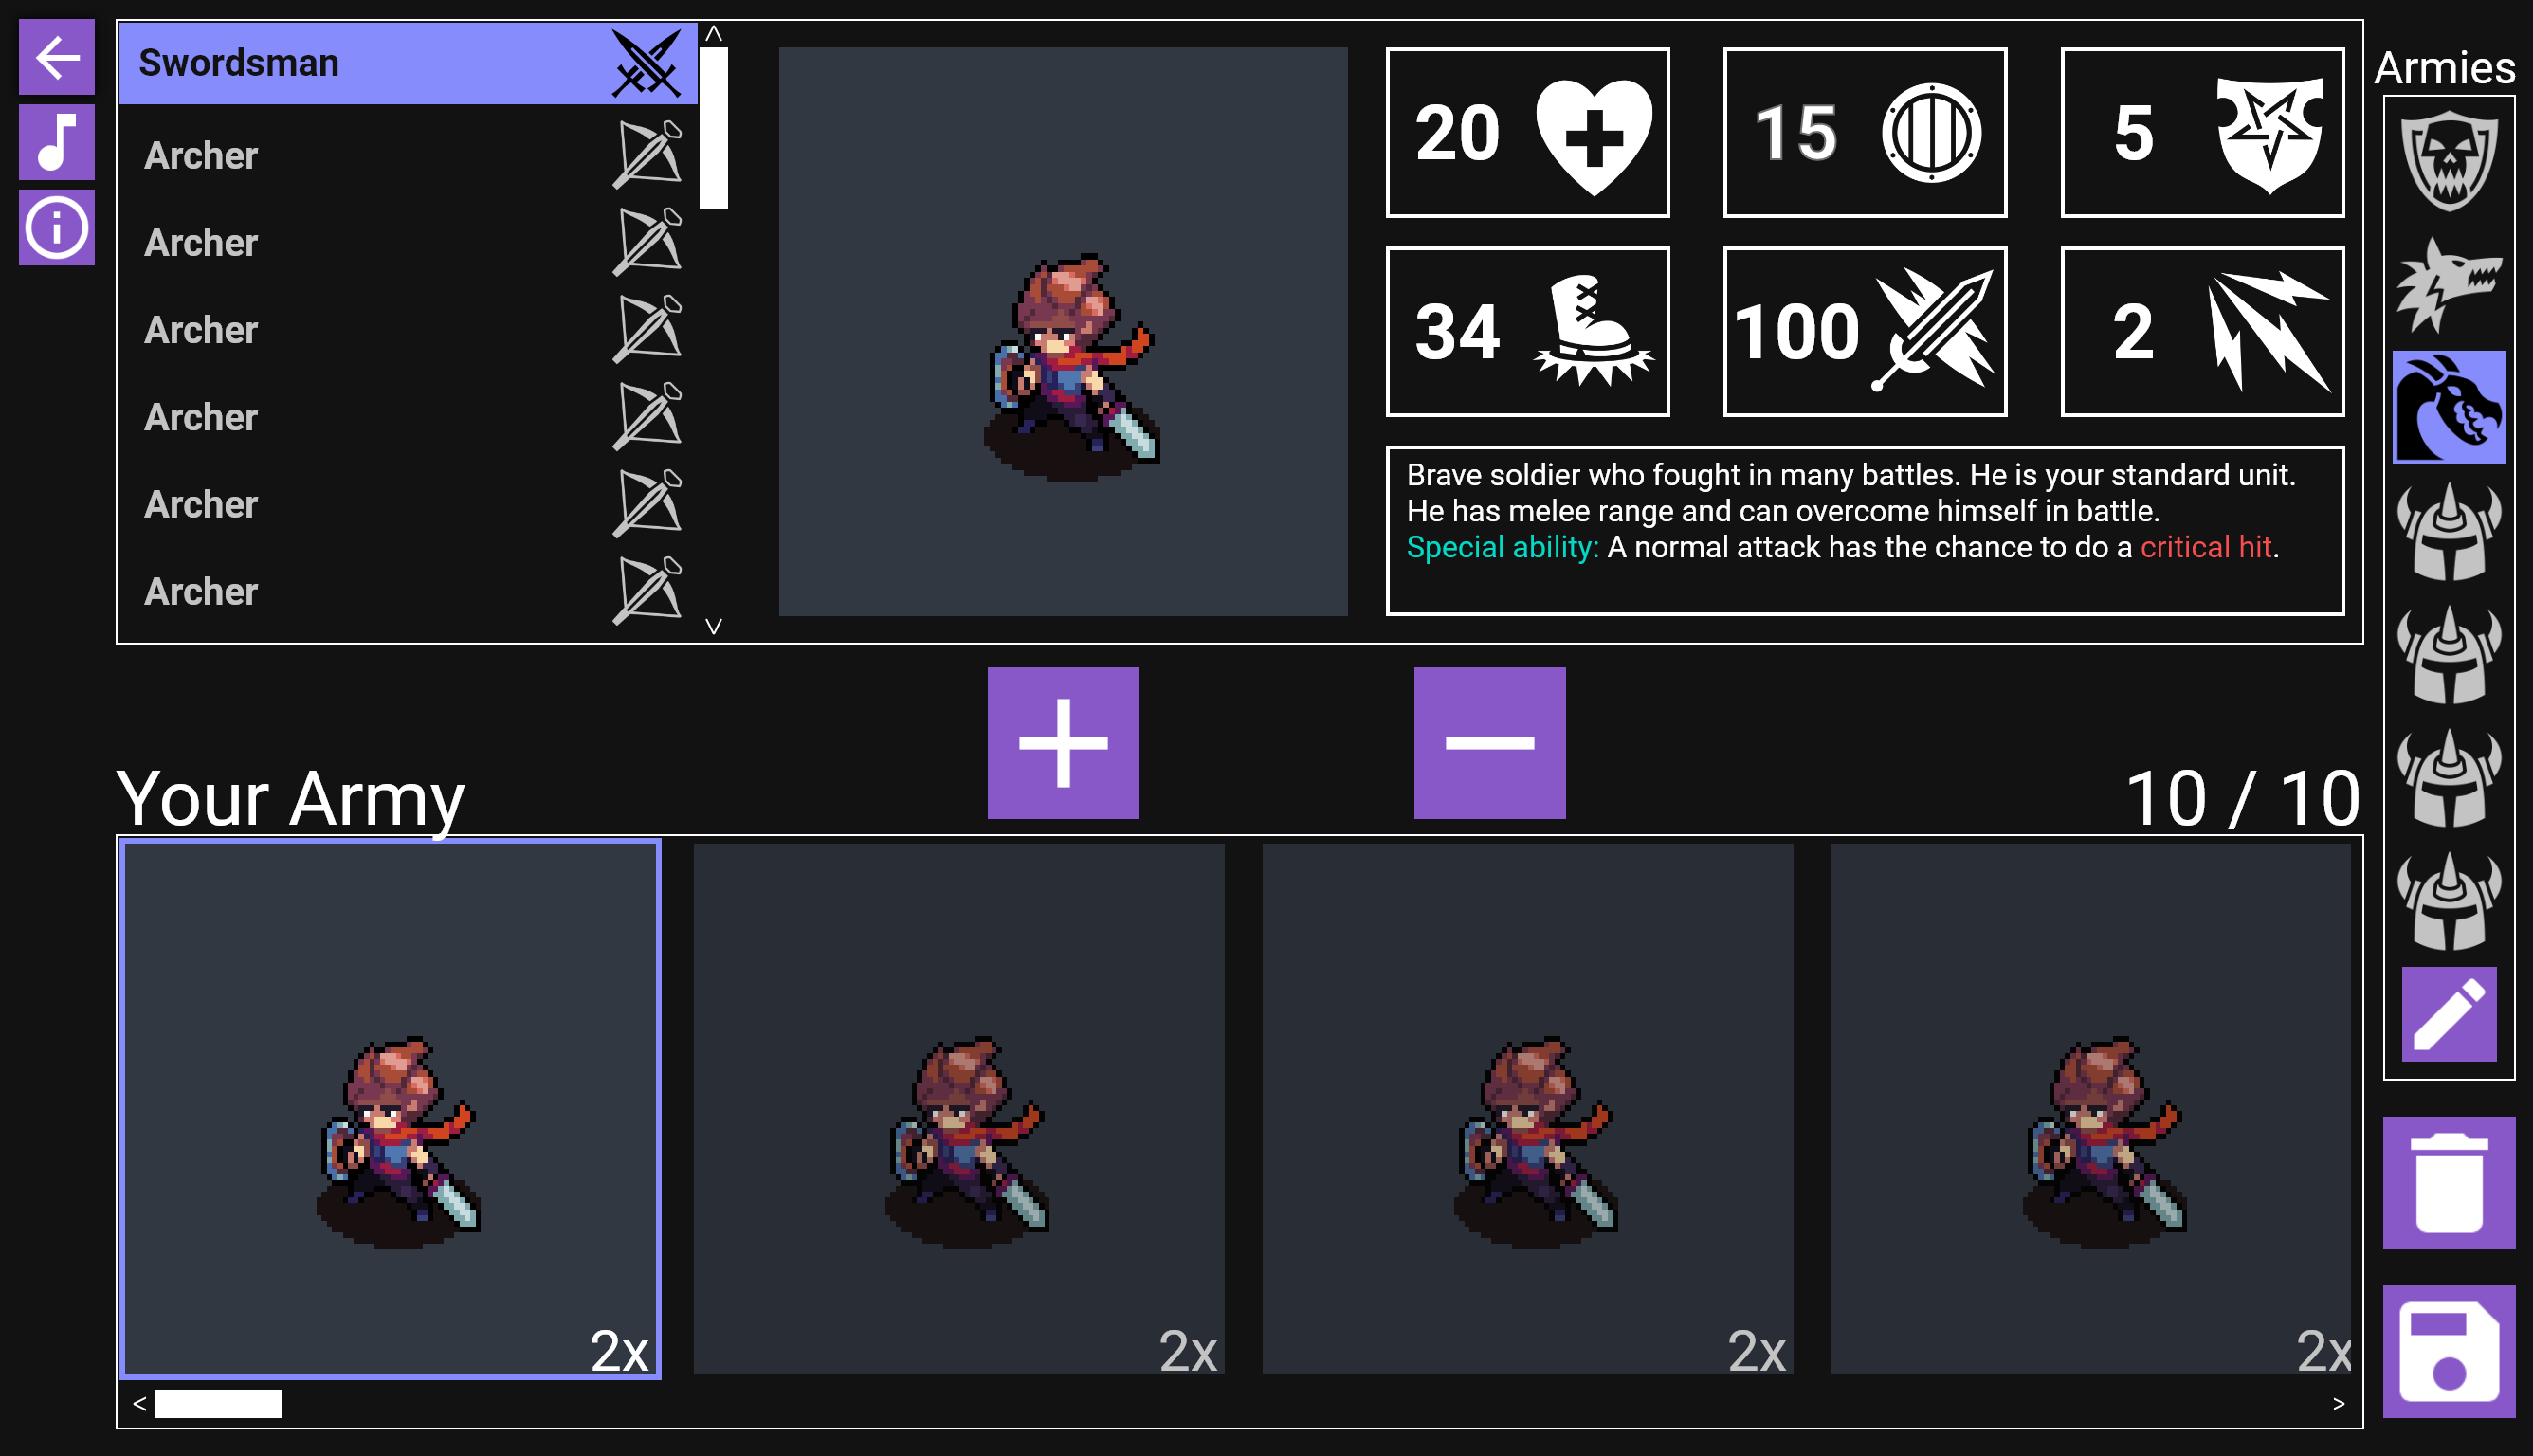
\includegraphics[width=0.7\textwidth]{ArmyBuilderMockUp.png}
				\caption{Mockup f�r den geplanten Armeemanager}
				\label{MockUpArmeemanager}
			\end{figure}
			
			\subsubsection{Implementaion} Die Umsetzung dieser Bereiche hat dabei fast 1:1 statt gefunden. Auf \Abb{ImplementierungArmeemanager} ist die abSchlie�ende Implemenation des Armeemangers zu sehen. Die Kernbereiche wurden wie geplant umgesetzt. Im Design und der Anordnung sind dabei leichte Unterschiede zu erkennen. Die Rahmen um die Einheitenauswahl und der Armeeauswahl sind entfallen, da dies zu einer �bersichtlicheren Oberfl�che beigetragen hat. Der Edit-Button zum �ndern der Armeeinformationen wurde aus der Armeeauswahl herausgezogen, um ihn in eine Reihe mit den anderen Buttons zu bringen. Der Detailansicht der Einheiten wurde eine Can Attack-Ansicht hinzugef�gt, da sich durch die erhaltenen Servernachrichten eine solche �bersicht als sinnvoll erwies.
			Es wurden noch die folgenden zus�tzlichen Features implementiert:
			\begin{itemize}
				\item Lore und Flavour f�r alle Einheiten
				\item Individuelle Armeeicons und Namen
				\item Clear\ Button zum schnellen \glqq aufr�umen\grqq von Armeen
				\item Indikator f�r das Speichern von Armeen
			\end{itemize}
			
			\begin{figure}[H] 
				\centering
				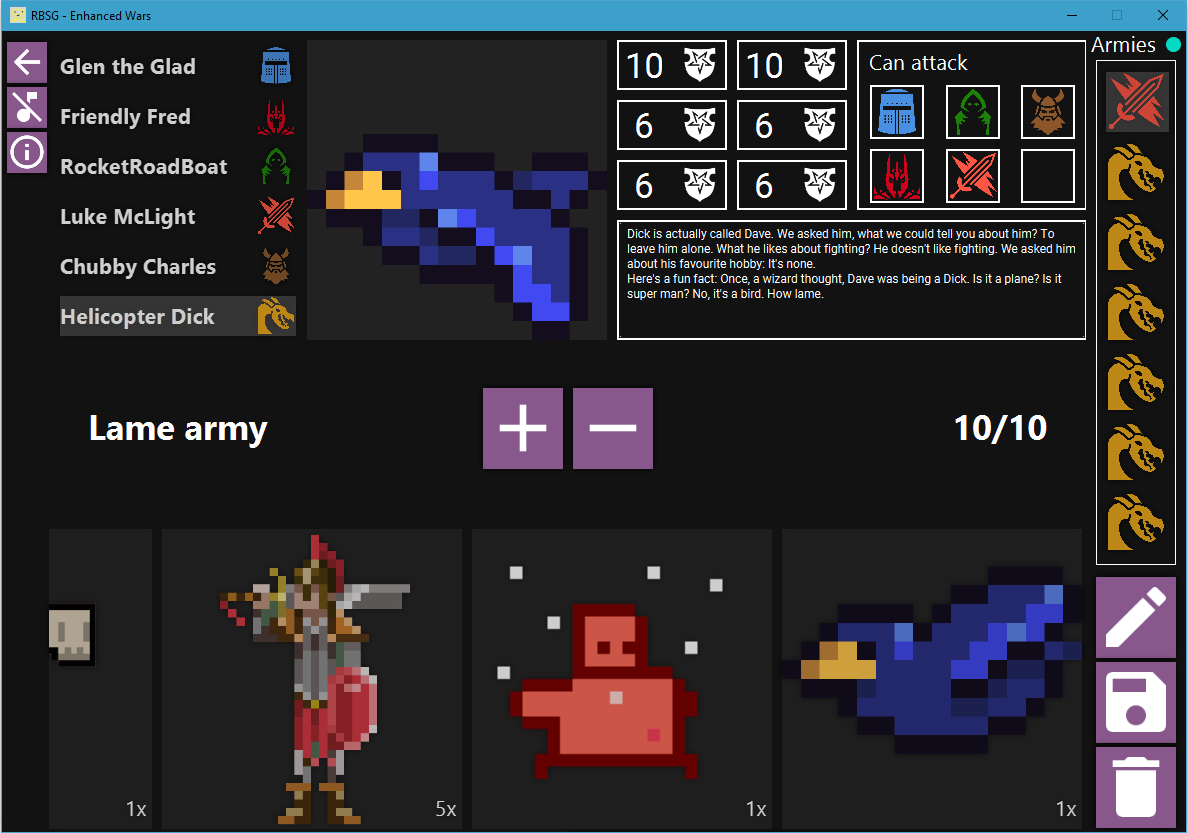
\includegraphics[width=0.7\textwidth]{ArmyBuilder_final.PNG}
				\caption{Realisierung des Armeemanagers am Ende von Release 2}
				\label{ImplementierungArmeemanager}
			\end{figure}
		
			\subsubsection{Armee-Editor}
			Im Kundengespr�ch zu Beginn des 2. Releases wurde vom Kunden noch die Anforderung gestellt die Icons der Armee individuell gestalten zu k�nnen. Daf�r wurde das Mockup in \Abb{ArmyEditorMockUp} erstellt. Die Umsetzung ist in \Abb{ArmyEditorImplementation} zu sehen. Die Implementierung unterscheidet sich vom Mockup nur in den Farben und den Schlie�en-Button. Der Schlie�en-Button wurde im Mockup vergessen und wurde in der Realisierung nachgetragen. Der farbliche Unterschied ist der zeitlichen Begrenzung geschuldet. Die Funktionalit�ten wurden vom Entwickler fertig gestellt, so ist es m�glich den Armeenamen zu bearbeiten und auch das Icon individuell aus einer vorgefertigten Liste auszuw�hlen. f�r den Design Aspekt fehlte am Ende des Releases die Zeit.
			
			\begin{figure}[H] 
				\centering
				\includegraphics[width=0.5\textwidth]{ArmyEditor.png}
				\caption{Mockup des Armee-Editor}
				\label{ArmyEditorMockUp}
			\end{figure}
		
			\begin{figure}[H] 
				\centering
				\includegraphics[width=0.5\textwidth]{ArmyEditor_final.PNG}
				\caption{Implementierung des Armee-Editor}
				\label{ArmyEditorImplementation}
			\end{figure}
		
			\subsubsection{Info zu den Attributen}
			Als zus�tzliches Feature wurde noch die eine �bersicht zu den Attributen erstellt, welche die Einheit besitzt. Die umgesetzte Oberfl�che ist in \Abb{AttributInfo} zu sehen. Geplant war die in \Abb{MockupAttribute} zu sehende Oberfl�che. Diese wurde so umgesetzt.
			
			\begin{figure}[H] 
				\centering
				\includegraphics[width=0.5\textwidth]{Attribute_Info_final.PNG}
				\caption{�bersicht f�r die Attribute der Einheiten}
				\label{AttributInfo}
			\end{figure}
		
			\begin{figure}[H] 
				\centering
				\includegraphics[width=0.5\textwidth]{InfoView.png}
				\caption{Mockup �bersicht �ber die Attribute}
				\label{MockupAttribute}
			\end{figure}
		
			\subsection{Warteraum}
			Zu Begin des zweiten Releases wurde ein Warteraum geplant, in welchen man nach Spielbeitritt kommt. Das Mockup ist in \Abb{MockupWaitingRoom} zu sehen. Es wurden fast alle geplanten Features im Warteraum umgesetzt, die Implementierung ist in \Abb{ImplementationWaitingRoom} zu sehen. Den Wartraum haben wir dabei in 3 Komponenten Unterteil:
			\begin{itemize}
				\item das Anzeigen der Spieler
				\item den Chat
				\item die Kartenvorschau
			\end{itemize}
			Diese Komponenten wurden auch wie geplant umgesetzt. Als Zusatz wird noch in den Spielerkarten die Farbe angezeigt, welcher ein Spieler f�r das kommende Spiel hat. Am rechten Rand sollte noch eine die Einheitenliste f�r die ausgew�hlte Armee angezeigt werden. Dieses Feature wurde nicht mehr umgesetzt, da es im n�chsten Release wieder verworfen worden w�re und wir uns so auf andere Sachen konzentriert haben.
			\begin{figure}[H] 
				\centering
				\includegraphics[width=0.7\textwidth]{Waiting_Room_Game_mit_ArmyView.png}
				\caption{Mockup des Warteraum}
				\label{MockupWaitingRoom}
			\end{figure}
			
			\begin{figure}[H] 
				\centering
				\includegraphics[width=0.7\textwidth]{WaitingRoom_final.PNG}
				\caption{Umsetzung des Warteraums im 2. Release}
				\label{ImplementationWaitingRoom}
			\end{figure}
			Damit sind auch folgende Anforderungen umgesetzt:
			\begin{itemize}
				\item Initiales Spielgeschehen anzeigen (indirekt �ber die Kartenvorschau)
				\item Spieler, die ein Spiel beitreten
				\item Von Spiel zur�ck in die Lobby gehen
				\item Ingame Chat
			\end{itemize}
			
			\subsection{Ingame}
			Als das 2. Release geplant wurde, war den Product Owner nicht bewusst, dass auch die Implementierung einer Karte zu diesem Release dazu geh�rt. Deshalb wurde kein Mockup f�r diese Situation angefertigt. Trotzdem war es uns m�glich eine Ingame Oberfl�che zu erstellen. Diese ist in \Abb{Ingame} zu sehen. Umgesetzt wurde hier:
			\begin{itemize}
				\item das Zeichnen der Karte
				\item das Zeichnen der Startpositionen der Einheiten
				\item Zoomen auf dem Spielfeld
				\item Verlassen des Ingames
			\end{itemize}
			\begin{figure}[H] 
				\centering
				\includegraphics[width=0.7\textwidth]{Ingame_final.PNG}
				\caption{Umsetzung der Ingame Oberfl�che im 2. Release}
				\label{Ingame}
			\end{figure}
			Durch die Implementierung der Ingame Oberfl�che wird die Anforderung das initiale Spielgeschehen anzuzeigen erf�llt. Es sollte auch m�glich sein, vom Spiel zur�ck in die Lobby zu gehen. Dies ist �ber den zur�ck-Button in der linken oberen Ecke m�glich. Das Zoomen wird �ber die zwei nebenliegenden Buttons realisiert. Bei einem Zwei-Spieler-Spiel ist ein 3-Stufiger Zoom m�glich und bei einem Vier-Spieler-Spiel ein 4-Stufen Zoom. Die Einheiten werden auf Ihren Startpositionen auf der Karte dargestellt. Eine Besonderheit bei der Darstellung der Karte ist, dass die �berg�nge zwischen Biomen fl�ssig ist. So werden bei �berg�nge andere Graphiken gew�hlt, um diese fl�ssig darzustellen.
			
			\subsection{Lobby}
			Die Lobby war von den Anforderungen dieses Releases nicht betroffen. Um jedoch ein angenehmeres Bedienverhalten zu gew�hrleisten, haben wir der Lobby noch eine Armeeauswahl hinzugef�gt, da eine Armee ben�tigt wird um einem Spiel beizutreten. Zu sehen ist die Umsetzung auf \Abb{LobbyFinal}. Die Icons der Armee werden dabei ,je nach Konfiguration, individuell dargestellt. Die Oberfl�che ist auch Responsive gehalten, so wird der ausgew�hlte Eintrag hervorgehoben. Ist keine Armee ausgew�hlt, so wird der Spiel erstellen-Button und auch die Spiel beitreten-Buttons deaktiviert.
			\begin{figure}[H] 
				\centering
				\includegraphics[width=0.7\textwidth]{Lobby_final.PNG}
				\caption{Lobby mit Armeeauswahl am Ende des 2. Releases}
				\label{LobbyFinal}
			\end{figure}
			
				\subsubsection{Spiel erstellen Formular}
				In diesen Release wurde auch das Spiel erstellen Formular optisch aufgearbeitet, dies kann man in \Abb{CreateGameFormularReworked} sehen. Es ist nun an das Dark Theme angepasst wurden.
				\begin{figure}[H] 
					\centering
					\includegraphics[width=0.7\textwidth]{Create_Game_final.PNG}
					\caption{Optisch �berarbeitetes \glqq Spiel erstellen\grqq Formular }
					\label{CreateGameFormularReworked}
				\end{figure}
			
			\subsection{Alerts}
			Im Verlauf des zweiten Releases entschieden wir uns dazu die Alters optische an unsere Thema anzupassen. Anfangs wurden die von JavaFX generierten Alters genutzt, diese sind in \Abb{AlertsOld} zu sehen. Diese wurden dann von uns durch die in \Abb{AlertsNew} zu sehenden Alerts ersetzt. Diese werden nun mit dem von uns erstellten Dark Theme dargestellt.AlertsNewAlertsNew
			\begin{figure}[H] 
				\centering
				\includegraphics[width=0.7\textwidth]{Alert_Old.PNG}
				\caption{Alerts von JavaFX}
				\label{AlertsOld}
			\end{figure}
		
			\begin{figure}[H] 
				\centering
				\includegraphics[width=0.7\textwidth]{Alerts_New_Style.PNG}
				\caption{�berarbeitet Alerts im Dark Theme}
				\label{AlertsNew}
			\end{figure} 
		
	\newpage
	\appendix
	\pagenumbering{Roman} 
	\listoffigures
	\listoftables
\end{document}